\chapter{Deep Learning in Structured Domains} \label{ch:deep-learning-structures}
A \keyword{structured domain} is a data domain whose elements are formed by a set of atomic \emph{entities}, and the \emph{relations} between them. Structured data is common in several fields, such as biology, chemistry, finance, social networks, and many more. Typical examples are sequences such as time-series data, hierarchical structures such as parse trees, and graphs representing molecular structures. One distinctive characteristic of structured data is that it has \keyword{variable size}, meaning that the number of entities composing the datum is not fixed in general. This constitutes a serious limitation for traditional \gls{ml} models, which are designed to work with \quotes{flat} data, \ie collections of fixed-size vectors. In this chapter, we present a class of \glspl{nn} that are able to handle variable-sized inputs for learning in structured domains.

\section{Graphs}\label{sec:graphs}
The elements of structured domains can be described in a compact and convenient notation using the general formalism of \keyword{graphs} \citep{bondy1976graph}. Informally, a graph is a collection of \emph{vertices} (the entities) connected through a collection of \emph{edges} (the relations). In the literature, vertices are sometimes called \emph{nodes}, while edges are also referred to as \emph{arcs} or \emph{links}. Formally, a graph with $n$ vertices is a pair
$$\Graph{g} =\langle \Nodes{g}, \Edges{g}\rangle,$$
where $\Nodes{g}= \Set{v_1, v_2, \ldots, v_n}$ is its set of vertices, and $\Edges{g} = \Set{\{u, v\} \mid u, v \in \Nodes{g}}$ is its set of edges. In a graph, $\Edges{g}$  specifies the graph \emph{structure}, that is, the way vertices are interconnected. Notice that the pair $\Set{u,v}$ is unordered: in this case, the graph is called \keyword{undirected}. Figure \ref{fig:undirected-graph} shows a visual representation of an undirected graph.
Given an edge $\Set{u, v} \in \Edges{g}$, $u$ and $v$ are called its \emph{endpoints}, and are said to be \emph{adjacent}. Alternatively, we say that $\Set{u, v}$ is \emph{incident} to $u$ and $v$. Edges of the form $\Set{v,v}$ that connect a vertex to itself are called \emph{self-loops}.
\begin{figure*}
    \begin{subfigure}[b]{0.38\linewidth}
        \centering
        \resizebox{.9\textwidth}{!}{

\tikzset{every picture/.style={line width=0.75pt}} %set default line width to 0.75pt

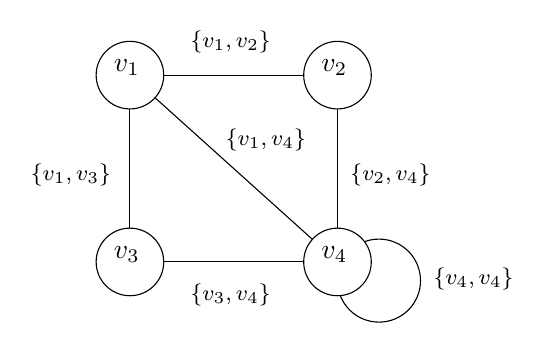
\begin{tikzpicture}[x=0.75pt,y=0.75pt,yscale=-1,xscale=1]
%uncomment if require: \path (0,178); %set diagram left start at 0, and has height of 178

%Shape: Circle [id:dp3051243428292618]
\draw   (180,140) .. controls (180,128.95) and (188.95,120) .. (200,120) .. controls (211.05,120) and (220,128.95) .. (220,140) .. controls (220,151.05) and (211.05,160) .. (200,160) .. controls (188.95,160) and (180,151.05) .. (180,140) -- cycle ;

% Text Node
\draw  [fill={rgb, 255:red, 255; green, 255; blue, 255 }  ,fill opacity=1 ]  (80, 41) circle [x radius= 16.28, y radius= 16.28]   ;
\draw (71,32.4) node [anchor=north west][inner sep=0.75pt]    {$v_{1}$};
% Text Node
\draw  [fill={rgb, 255:red, 255; green, 255; blue, 255 }  ,fill opacity=1 ]  (180, 41) circle [x radius= 16.28, y radius= 16.28]   ;
\draw (171,32.4) node [anchor=north west][inner sep=0.75pt]    {$v_{2}$};
% Text Node
\draw  [fill={rgb, 255:red, 255; green, 255; blue, 255 }  ,fill opacity=1 ]  (80, 131) circle [x radius= 16.28, y radius= 16.28]   ;
\draw (71,122.4) node [anchor=north west][inner sep=0.75pt]    {$v_{3}$};
% Text Node
\draw  [fill={rgb, 255:red, 255; green, 255; blue, 255 }  ,fill opacity=1 ]  (180, 131) circle [x radius= 16.28, y radius= 16.28]   ;
\draw (171,122.4) node [anchor=north west][inner sep=0.75pt]    {$v_{4}$};
% Text Node
\draw (31,82.4) node [anchor=north west][inner sep=0.75pt]  [font=\footnotesize]  {$\{v_{1} ,v_{3}\}$};
% Text Node
\draw (185,82.4) node [anchor=north west][inner sep=0.75pt]  [font=\footnotesize]  {$\{v_{2} ,v_{4}\}$};
% Text Node
\draw (225,132.4) node [anchor=north west][inner sep=0.75pt]  [font=\footnotesize]  {$\{v_{4} ,v_{4}\}$};
% Text Node
\draw (108,140.4) node [anchor=north west][inner sep=0.75pt]  [font=\footnotesize]  {$\{v_{3} ,v_{4}\}$};
% Text Node
\draw (108,18.4) node [anchor=north west][inner sep=0.75pt]  [font=\footnotesize]  {$\{v_{1} ,v_{2}\}$};
% Text Node
\draw (125,65.4) node [anchor=north west][inner sep=0.75pt]  [font=\footnotesize]  {$\{v_{1} ,v_{4}\}$};
% Connection
\draw    (80,57.28) -- (80,114.72) ;
% Connection
\draw    (96.28,41) -- (163.72,41) ;
% Connection
\draw    (180,57.28) -- (180,114.72) ;
% Connection
\draw    (96.28,131) -- (163.72,131) ;
% Connection
\draw    (92.1,51.89) -- (167.9,120.11) ;

\end{tikzpicture}}
        \caption{An undirected graph.}
        \label{fig:undirected-graph}
    \end{subfigure}
    \begin{subfigure}[b]{0.32\linewidth}
        \centering
        \resizebox{.9\textwidth}{!}{

\tikzset{every picture/.style={line width=0.75pt}} %set default line width to 0.75pt        

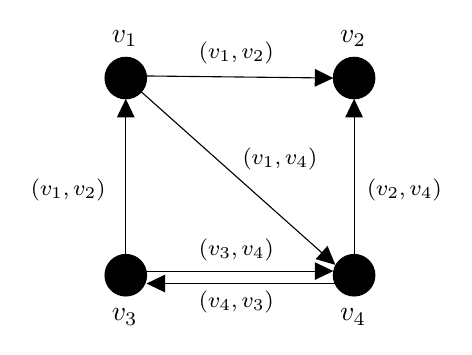
\begin{tikzpicture}[x=0.75pt,y=0.75pt,yscale=-1,xscale=1]
%uncomment if require: \path (0,186); %set diagram left start at 0, and has height of 186

%Straight Lines [id:da7523828398029215] 
\draw    (70,40) -- (157,40.97) ;
\draw [shift={(160,41)}, rotate = 180.64] [fill={rgb, 255:red, 0; green, 0; blue, 0 }  ][line width=0.08]  [draw opacity=0] (8.93,-4.29) -- (0,0) -- (8.93,4.29) -- cycle    ;
%Straight Lines [id:da6810560947997366] 
\draw    (60,134) -- (60,54) ;
\draw [shift={(60,51)}, rotate = 450] [fill={rgb, 255:red, 0; green, 0; blue, 0 }  ][line width=0.08]  [draw opacity=0] (8.93,-4.29) -- (0,0) -- (8.93,4.29) -- cycle    ;
%Straight Lines [id:da13593621053018157] 
\draw    (60,41) -- (158.76,129) ;
\draw [shift={(161,131)}, rotate = 221.7] [fill={rgb, 255:red, 0; green, 0; blue, 0 }  ][line width=0.08]  [draw opacity=0] (8.93,-4.29) -- (0,0) -- (8.93,4.29) -- cycle    ;
%Straight Lines [id:da7020714410789375] 
\draw    (170,130) -- (170,54) ;
\draw [shift={(170,51)}, rotate = 450] [fill={rgb, 255:red, 0; green, 0; blue, 0 }  ][line width=0.08]  [draw opacity=0] (8.93,-4.29) -- (0,0) -- (8.93,4.29) -- cycle    ;
%Shape: Circle [id:dp03304258230702484] 
\draw  [color={rgb, 255:red, 0; green, 0; blue, 0 }  ,draw opacity=1 ][fill={rgb, 255:red, 0; green, 0; blue, 0 }  ,fill opacity=1 ] (160,136) .. controls (160,130.48) and (164.48,126) .. (170,126) .. controls (175.52,126) and (180,130.48) .. (180,136) .. controls (180,141.52) and (175.52,146) .. (170,146) .. controls (164.48,146) and (160,141.52) .. (160,136) -- cycle ;
%Shape: Circle [id:dp7633189619087324] 
\draw  [color={rgb, 255:red, 0; green, 0; blue, 0 }  ,draw opacity=1 ][fill={rgb, 255:red, 0; green, 0; blue, 0 }  ,fill opacity=1 ] (50,136) .. controls (50,130.48) and (54.48,126) .. (60,126) .. controls (65.52,126) and (70,130.48) .. (70,136) .. controls (70,141.52) and (65.52,146) .. (60,146) .. controls (54.48,146) and (50,141.52) .. (50,136) -- cycle ;
%Shape: Circle [id:dp47599843876160874] 
\draw  [color={rgb, 255:red, 0; green, 0; blue, 0 }  ,draw opacity=1 ][fill={rgb, 255:red, 0; green, 0; blue, 0 }  ,fill opacity=1 ] (160,41) .. controls (160,35.48) and (164.48,31) .. (170,31) .. controls (175.52,31) and (180,35.48) .. (180,41) .. controls (180,46.52) and (175.52,51) .. (170,51) .. controls (164.48,51) and (160,46.52) .. (160,41) -- cycle ;
%Shape: Circle [id:dp8036256762510467] 
\draw  [color={rgb, 255:red, 0; green, 0; blue, 0 }  ,draw opacity=1 ][fill={rgb, 255:red, 0; green, 0; blue, 0 }  ,fill opacity=1 ] (50,41) .. controls (50,35.48) and (54.48,31) .. (60,31) .. controls (65.52,31) and (70,35.48) .. (70,41) .. controls (70,46.52) and (65.52,51) .. (60,51) .. controls (54.48,51) and (50,46.52) .. (50,41) -- cycle ;
%Straight Lines [id:da523220310179759] 
\draw    (60,134) -- (157,134) ;
\draw [shift={(160,134)}, rotate = 180] [fill={rgb, 255:red, 0; green, 0; blue, 0 }  ][line width=0.08]  [draw opacity=0] (8.93,-4.29) -- (0,0) -- (8.93,4.29) -- cycle    ;
%Straight Lines [id:da5511445342877679] 
\draw    (170,140) -- (73,140) ;
\draw [shift={(70,140)}, rotate = 360] [fill={rgb, 255:red, 0; green, 0; blue, 0 }  ][line width=0.08]  [draw opacity=0] (8.93,-4.29) -- (0,0) -- (8.93,4.29) -- cycle    ;

% Text Node
\draw (52,17) node [anchor=north west][inner sep=0.75pt]    {$v_{1}$};
% Text Node
\draw (162,17) node [anchor=north west][inner sep=0.75pt]    {$v_{2}$};
% Text Node
\draw (52,151) node [anchor=north west][inner sep=0.75pt]    {$v_{3}$};
% Text Node
\draw (162,151) node [anchor=north west][inner sep=0.75pt]    {$v_{4}$};
% Text Node
\draw (94,22.4) node [anchor=north west][inner sep=0.75pt]  [font=\footnotesize]  {$( v_{1} ,v_{2})$};
% Text Node
\draw (115,73.4) node [anchor=north west][inner sep=0.75pt]  [font=\footnotesize]  {$( v_{1} ,v_{4})$};
% Text Node
\draw (175,88.4) node [anchor=north west][inner sep=0.75pt]  [font=\footnotesize]  {$( v_{2} ,v_{4})$};
% Text Node
\draw (13,88.4) node [anchor=north west][inner sep=0.75pt]  [font=\footnotesize]  {$( v_{1} ,v_{2})$};
% Text Node
\draw (94,117.4) node [anchor=north west][inner sep=0.75pt]  [font=\footnotesize]  {$( v_{3} ,v_{4})$};
% Text Node
\draw (94,142.4) node [anchor=north west][inner sep=0.75pt]  [font=\footnotesize]  {$( v_{4} ,v_{3})$};


\end{tikzpicture}}
        \caption{A directed graph.}
        \label{fig:directed-graph}
    \end{subfigure}
    \begin{subfigure}[b]{0.25\linewidth}
        \centering
        \resizebox{.9\textwidth}{!}{

\tikzset{every picture/.style={line width=0.75pt}} %set default line width to 0.75pt

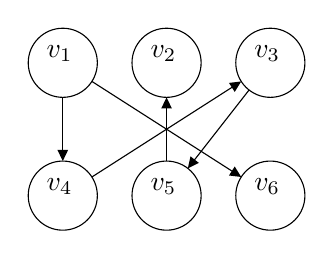
\begin{tikzpicture}[x=0.75pt,y=0.75pt,yscale=-1,xscale=1]
%uncomment if require: \path (0,134); %set diagram left start at 0, and has height of 134


% Text Node
\draw    (54, 100.5) circle [x radius= 16.65, y radius= 16.65]   ;
\draw (45,91) node [anchor=north west][inner sep=0.75pt]   [align=left] {$\displaystyle v_{4}$};
% Text Node
\draw    (104, 100.5) circle [x radius= 16.65, y radius= 16.65]   ;
\draw (95,91) node [anchor=north west][inner sep=0.75pt]   [align=left] {$\displaystyle v_{5}$};
% Text Node
\draw    (154, 100.5) circle [x radius= 16.65, y radius= 16.65]   ;
\draw (145,91) node [anchor=north west][inner sep=0.75pt]   [align=left] {$\displaystyle v_{6}$};
% Text Node
\draw    (54, 36.5) circle [x radius= 16.65, y radius= 16.65]   ;
\draw (45,27) node [anchor=north west][inner sep=0.75pt]   [align=left] {$\displaystyle v_{1}$};
% Text Node
\draw    (104, 36.5) circle [x radius= 16.65, y radius= 16.65]   ;
\draw (95,27) node [anchor=north west][inner sep=0.75pt]   [align=left] {$\displaystyle v_{2}$};
% Text Node
\draw    (154, 36.5) circle [x radius= 16.65, y radius= 16.65]   ;
\draw (145,27) node [anchor=north west][inner sep=0.75pt]   [align=left] {$\displaystyle v_{3}$};
% Connection
\draw    (54,53.15) -- (54,80.85) ;
\draw [shift={(54,83.85)}, rotate = 270] [fill={rgb, 255:red, 0; green, 0; blue, 0 }  ][line width=0.08]  [draw opacity=0] (5.36,-2.57) -- (0,0) -- (5.36,2.57) -- cycle    ;
% Connection
\draw    (68.03,45.48) -- (137.45,89.91) ;
\draw [shift={(139.97,91.52)}, rotate = 212.62] [fill={rgb, 255:red, 0; green, 0; blue, 0 }  ][line width=0.08]  [draw opacity=0] (5.36,-2.57) -- (0,0) -- (5.36,2.57) -- cycle    ;
% Connection
\draw    (68.03,91.52) -- (137.45,47.09) ;
\draw [shift={(139.97,45.48)}, rotate = 507.38] [fill={rgb, 255:red, 0; green, 0; blue, 0 }  ][line width=0.08]  [draw opacity=0] (5.36,-2.57) -- (0,0) -- (5.36,2.57) -- cycle    ;
% Connection
\draw    (104,83.85) -- (104,56.15) ;
\draw [shift={(104,53.15)}, rotate = 450] [fill={rgb, 255:red, 0; green, 0; blue, 0 }  ][line width=0.08]  [draw opacity=0] (5.36,-2.57) -- (0,0) -- (5.36,2.57) -- cycle    ;
% Connection
\draw    (143.75,49.62) -- (116.1,85.01) ;
\draw [shift={(114.25,87.38)}, rotate = 308] [fill={rgb, 255:red, 0; green, 0; blue, 0 }  ][line width=0.08]  [draw opacity=0] (5.36,-2.57) -- (0,0) -- (5.36,2.57) -- cycle    ;

\end{tikzpicture}}
        \caption{A bipartite graph.}
        \label{fig:bipartite-graph}
    \end{subfigure}
    \caption{Three examples of graphs.}
\end{figure*}
Graphs where it is possible to have more than one edge between a pair of vertices are called \emph{multigraphs}. In this work, we restrict ourselves to the case where there is at most one possible edge between two vertices.

\paragraph{Directed Graphs}
A \keyword{directed graph} is one where the edges are ordered pairs of vertices, or equivalently one where $\Edges{g}\subseteq \Nodes{g}\times \Nodes{g}$. A directed edge is written as $(u, v)$, meaning that it goes from vertex $u$ to vertex $v$. An example of directed graph is shown in Figure \ref{fig:directed-graph}. Given a directed graph $\Graph{g}$ and one of its vertices $v \in \Nodes{g}$, the set of all vertices from which an edge reaches $v$ is called \emph{predecessors} set, and is defined as $\Pred(v) = \Set{u \in \Nodes{g} \mid (u,v) \in \Edges{g}}$. The cardinality of the predecessors set is called the \emph{in-degree} of the vertex, and we indicate it as $\Fun{degree}_{in}(v)$. Analogously, the set of all vertices reached by an edge from $v$ is called the \emph{successors} set, and is defined as $\Succ(v) = \Set{u \in \Nodes{g}\mid (v,u) \in \Edges{g}}$. Its cardinality is called the \emph{out-degree} of the vertex, and indicated as $\Fun{degree}_{out}(v)$. The \emph{neighborhood} (or \emph{adjacency set}) of a vertex $v$ is the union of the predecessors and successors sets: $\Neigh(v) = \Pred(v) \bigcup \Succ(v)$. Alternatively, one can view the neighborhood as a function $\Neigh: \Nodes{g}\shortrightarrow 2^{\Nodes{g}}$ from vertices to sets of vertices. The cardinality of the neighborhood is called the \keyword{degree} of the vertex, indicated as $\Fun{degree}(v)$.  In this work, we consider all graphs directed unless otherwise specified. Undirected graphs are thus implicitly transformed into directed graphs with the same vertices, where the set of edges contains the edges $(v,u)$ and $(u,v)$ if and only if $\{u,v\}$ is an edge of the undirected graph.

\paragraph{Bipartite Graphs}
A graph $\Graph{g}$ is called \keyword{bipartite} if we can split $\Nodes{g}$ in two disjoint subsets $\Nodes{g}^{+}$ and $\Nodes{g}^{-}$, such that $(u, v) \in \Edges{g}$ if and only if either $u \in \Nodes{g}^{+}$ and $v \in \Nodes{g}^{-}$, or alternatively $v \in \Nodes{g}^{+}$ and $u \in \Nodes{g}^{-}$. Figure \ref{fig:bipartite-graph} shows an example of bipartite graph, where
$\Nodes{g}^{+} = \Set{v_1, v_2, v_3}$ and $\Nodes{g}^{-} = \Set{v_4, v_5, v_6}$.

\paragraph{Walks, Paths, and Cycles}
Let $\Graph{g}$ be a graph. A \emph{walk} of length $l$ is any sequence of $l$ vertices $\Par{v_1, v_2, \ldots, v_l}$, where each pair of consecutive vertices is adjacent, \ie $\Par{v_i, v_{i+1}} \in \Edges{g}$, $\forall i= 1, \ldots, i-1$. A \emph{path} of length $l$ from vertex $u$ to vertex $v$ is a walk such that $v_1 = u$ and $v_l = v$, where each vertex appears exactly once. If, given two vertices $u, v \in \Nodes{g}$ such that $u \neq v$, there exists a path between them, we say they are \emph{connected}, or that $v$ is reachable from $u$. Otherwise, we say they are \emph{disconnected}, or that $v$ is unreachable from $u$. The \emph{shortest path} from a node $u$ to a node $v$ is the path, among all paths from $u$ to $v$, with the smallest length. We indicate it with the notation $\Path{u}{g}{v}$. A graph is called \emph{connected} if every vertex is connected to any other vertex (ignoring the direction of the edges); otherwise it is called \emph{disconnected}. A \emph{cycle}, or \emph{loop}, of length $l$ is a walk where $v_1 = v_l$, and all the other vertices appear once in the sequence. Graphs that do not contain cycles are called \emph{acyclic}.

\paragraph{Trees and Sequences}
A graph $\Tree{t}$ is called a \keyword{tree} if its set of edges defines a \emph{partial order} over the set of vertices, implying that it is also connected and acyclic. The vertices of a tree are called \emph{nodes}. Given an edge $(u, v) \in \Edges{t}$, we call $u$ the \emph{parent} of $v$ and $v$ the \emph{child} of $u$. The set of children of a node $v$ is indicated with the notation $\Fun{ch}(v)$. In a tree, every node has exactly one parent, except for a node called \emph{root} or \emph{supersource}, which has no parent node. A tree is \emph{positional} if we can distinguish among the children of a node, \ie if there exist a consistent ordering between them. For example, in \emph{binary} trees (such as the one in Figure \ref{fig:tree}), each node can have a left and right child. Trees have a recursive structure: every node $v \in \Nodes{t}$ is itself the root of a tree, called \emph{sub-tree of} $\Tree{t}$ \emph{rooted at v}, and indicated as $\Tree{t}_v$. If $\Nodes{\Tree{t}_v}$ contains only $v$, $v$ is called a \emph{leaf}. Trees are useful to encode \emph{hierarchical} relationships among nodes.

A graph $\Seq{s}$ with $n$ vertices is called a \emph{sequential graph}, or \keyword{sequence} of length $n$, if its set of edges defines a \emph{total order} over the set of vertices, which allows us to represent the set of vertices in an ordered fashion as $\Nodes{s} = (v_1, v_2, \ldots, v_n)$. In a sequence, the vertices are usually called \emph{elements}. A sequence can be viewed as a special case of tree with only one leaf. Sequences are useful to encode \emph{sequential} relationships among elements; Figure \ref{fig:sequence} shows an example of a sequence of four elements.
\begin{figure*}
    \begin{subfigure}[b]{0.60\linewidth}
        \centering
        \resizebox{.8\textwidth}{!}{

\tikzset{every picture/.style={line width=0.75pt}} %set default line width to 0.75pt        

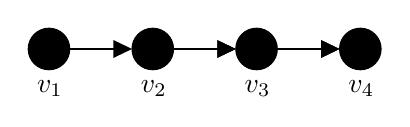
\begin{tikzpicture}[x=0.75pt,y=0.75pt,yscale=-1,xscale=1]
%uncomment if require: \path (0,54); %set diagram left start at 0, and has height of 54

%Shape: Circle [id:dp5966637236046903] 
\draw  [fill={rgb, 255:red, 0; green, 0; blue, 0 }  ,fill opacity=1 ] (10,20) .. controls (10,14.48) and (14.48,10) .. (20,10) .. controls (25.52,10) and (30,14.48) .. (30,20) .. controls (30,25.52) and (25.52,30) .. (20,30) .. controls (14.48,30) and (10,25.52) .. (10,20) -- cycle ;
%Straight Lines [id:da052084780507878126] 
\draw    (20,20) -- (57,20) ;
\draw [shift={(60,20)}, rotate = 180] [fill={rgb, 255:red, 0; green, 0; blue, 0 }  ][line width=0.08]  [draw opacity=0] (8.93,-4.29) -- (0,0) -- (8.93,4.29) -- cycle    ;
%Shape: Circle [id:dp5200693045335503] 
\draw  [fill={rgb, 255:red, 0; green, 0; blue, 0 }  ,fill opacity=1 ] (60,20) .. controls (60,14.48) and (64.48,10) .. (70,10) .. controls (75.52,10) and (80,14.48) .. (80,20) .. controls (80,25.52) and (75.52,30) .. (70,30) .. controls (64.48,30) and (60,25.52) .. (60,20) -- cycle ;
%Straight Lines [id:da33269281061881717] 
\draw    (70,20) -- (107,20) ;
\draw [shift={(110,20)}, rotate = 180] [fill={rgb, 255:red, 0; green, 0; blue, 0 }  ][line width=0.08]  [draw opacity=0] (8.93,-4.29) -- (0,0) -- (8.93,4.29) -- cycle    ;
%Straight Lines [id:da9716435563701427] 
\draw    (70,20) -- (107,20) ;
\draw [shift={(110,20)}, rotate = 180] [fill={rgb, 255:red, 0; green, 0; blue, 0 }  ][line width=0.08]  [draw opacity=0] (8.93,-4.29) -- (0,0) -- (8.93,4.29) -- cycle    ;
%Shape: Circle [id:dp3815536377212252] 
\draw  [fill={rgb, 255:red, 0; green, 0; blue, 0 }  ,fill opacity=1 ] (110,20) .. controls (110,14.48) and (114.48,10) .. (120,10) .. controls (125.52,10) and (130,14.48) .. (130,20) .. controls (130,25.52) and (125.52,30) .. (120,30) .. controls (114.48,30) and (110,25.52) .. (110,20) -- cycle ;
%Straight Lines [id:da660694621597677] 
\draw    (120,20) -- (157,20) ;
\draw [shift={(160,20)}, rotate = 180] [fill={rgb, 255:red, 0; green, 0; blue, 0 }  ][line width=0.08]  [draw opacity=0] (8.93,-4.29) -- (0,0) -- (8.93,4.29) -- cycle    ;
%Straight Lines [id:da23904459539502287] 
\draw    (120,20) -- (157,20) ;
\draw [shift={(160,20)}, rotate = 180] [fill={rgb, 255:red, 0; green, 0; blue, 0 }  ][line width=0.08]  [draw opacity=0] (8.93,-4.29) -- (0,0) -- (8.93,4.29) -- cycle    ;
%Shape: Circle [id:dp3652036582720466] 
\draw  [fill={rgb, 255:red, 0; green, 0; blue, 0 }  ,fill opacity=1 ] (160,20) .. controls (160,14.48) and (164.48,10) .. (170,10) .. controls (175.52,10) and (180,14.48) .. (180,20) .. controls (180,25.52) and (175.52,30) .. (170,30) .. controls (164.48,30) and (160,25.52) .. (160,20) -- cycle ;

% Text Node
\draw (13,34) node [anchor=north west][inner sep=0.75pt]    {$v_1$};
% Text Node
\draw (63,34) node [anchor=north west][inner sep=0.75pt]    {$v_2$};
% Text Node
\draw (113,34) node [anchor=north west][inner sep=0.75pt]    {$v_3$};
% Text Node
\draw (163,34) node [anchor=north west][inner sep=0.75pt]   {$v_4$};


\end{tikzpicture}}
        \caption{A sequence.}
        \label{fig:sequence}
    \end{subfigure}
    \begin{subfigure}[b]{0.39\linewidth}
        \centering
        \resizebox{.70\textwidth}{!}{

\tikzset{every picture/.style={line width=0.75pt}} %set default line width to 0.75pt

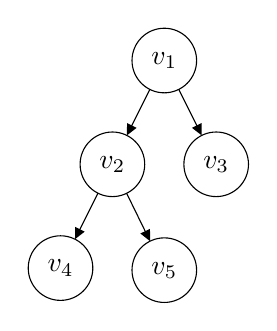
\begin{tikzpicture}[x=0.75pt,y=0.75pt,yscale=-1,xscale=1]
%uncomment if require: \path (0,151); %set diagram left start at 0, and has height of 151


% Text Node
\draw    (80, 20) circle [x radius= 15.56, y radius= 15.56]   ;
\draw (80,20) node   [align=left] {\begin{minipage}[lt]{13.600000000000001pt}\setlength\topsep{0pt}
\begin{center}
$\displaystyle v_{1}$
\end{center}

\end{minipage}};
% Text Node
\draw    (55, 70) circle [x radius= 15.56, y radius= 15.56]   ;
\draw (55,70) node   [align=left] {\begin{minipage}[lt]{13.600000000000001pt}\setlength\topsep{0pt}
\begin{center}
$\displaystyle v_{2}$
\end{center}

\end{minipage}};
% Text Node
\draw    (105, 70) circle [x radius= 15.56, y radius= 15.56]   ;
\draw (105,70) node   [align=left] {\begin{minipage}[lt]{13.600000000000001pt}\setlength\topsep{0pt}
\begin{center}
$\displaystyle v_{3}$
\end{center}

\end{minipage}};
% Text Node
\draw    (30, 120) circle [x radius= 15.56, y radius= 15.56]   ;
\draw (30,120) node   [align=left] {\begin{minipage}[lt]{13.600000000000001pt}\setlength\topsep{0pt}
\begin{center}
$\displaystyle v_{4}$
\end{center}

\end{minipage}};
% Text Node
\draw    (80, 121) circle [x radius= 15.56, y radius= 15.56]   ;
\draw (80,121) node   [align=left] {\begin{minipage}[lt]{13.600000000000001pt}\setlength\topsep{0pt}
\begin{center}
$\displaystyle v_{5}$
\end{center}

\end{minipage}};
% Connection
\draw    (73.04,33.92) -- (63.3,53.4) ;
\draw [shift={(61.96,56.08)}, rotate = 296.57] [fill={rgb, 255:red, 0; green, 0; blue, 0 }  ][line width=0.08]  [draw opacity=0] (5.36,-2.57) -- (0,0) -- (5.36,2.57) -- cycle    ;
% Connection
\draw    (48.04,83.92) -- (38.3,103.4) ;
\draw [shift={(36.96,106.08)}, rotate = 296.57] [fill={rgb, 255:red, 0; green, 0; blue, 0 }  ][line width=0.08]  [draw opacity=0] (5.36,-2.57) -- (0,0) -- (5.36,2.57) -- cycle    ;
% Connection
\draw    (61.85,83.97) -- (71.83,104.33) ;
\draw [shift={(73.15,107.03)}, rotate = 243.89] [fill={rgb, 255:red, 0; green, 0; blue, 0 }  ][line width=0.08]  [draw opacity=0] (5.36,-2.57) -- (0,0) -- (5.36,2.57) -- cycle    ;
% Connection
\draw    (86.96,33.92) -- (96.7,53.4) ;
\draw [shift={(98.04,56.08)}, rotate = 243.43] [fill={rgb, 255:red, 0; green, 0; blue, 0 }  ][line width=0.08]  [draw opacity=0] (5.36,-2.57) -- (0,0) -- (5.36,2.57) -- cycle    ;

\end{tikzpicture}}
        \caption{A tree.}
        \label{fig:tree}
    \end{subfigure}
    \caption{Special classes of graphs.}
\end{figure*}

\paragraph{Subgraphs and Induced Subgraphs} A \keyword{subgraph}
$\Graph{h} = \langle \Nodes{h}, \Edges{h} \rangle$ of a graph $\Graph{g}$ is any graph for which $\Nodes{h} \subseteq \Nodes{g}$ and  $\Edges{h} \subseteq \Edges{g}$. If $\Edges{h} = (\Nodes{h} \times \Nodes{h}) \Inter \Edges{g}$, or equivalently, if $\Nodes{h}$ contains only vertices that are endpoints in $\Edges{g}$, the resulting subgraph is called \keyword{induced subgraph}. We indicate the subgraph of $\Graph{g}$ induced by $\Graph{h}$ with the notation $\InducedSubgraph{g}{\Graph{h}}$.

\subsection{Attributed Graphs} \label{sec:attr-graphs}
Real-world instances of graphs usually carry out other information besides structure, generally attached to their vertices or edges. As an example, consider the graph representation of a molecule, in which vertices are usually annotated with an atom type, and edges are annotated with a chemical bond type. Given a graph $\Graph{g}$ with $n$ vertices and $m$ edges, we define the associated graph with additional information content, and we call it an \keyword{attributed graph}, as a triplet $\langle \Graph{g}, \chi, \xi \rangle,$ where $\chi: \Nodes{g} \rightarrow \Real^d$ is a mapping from the space of vertices to a space of $d$-dimensional \emph{vertex features}, and $\xi: \Edges{g}\rightarrow \Real^{e}$, is a mapping from the space of edges to a space of $e$-dimensional \emph{edge features}. The values of these features can be either discrete (in which case the features are called \emph{labels} and encoded as one-hot vectors) or continuous vectors. In most cases, we omit to define $\chi$ and $\xi$ explicitly, and provide the vertex and edge features directly as sets, \eg $\Vector{x}_{\Graph{g}}= \Set{\Elem{x}{v} \in \Real^d \mid v \in \Nodes{g}}$ for the vertex features, and $\Vector{e}_{\Graph{g}} = \Set{\Elem{e}{u,v} \in \Real^e \mid (u, v) \in \Edges{g}}$ for the edge features. In this case, an attributed graph is a triplet:
$$\AttrGraph{g} = \VectorGraph{x}{g}.$$
If some ordering of the vertices and edges is assumed, we can represent equivalently $\chi$ as a matrix $\Matrix{X}_{\Graph{g}} \in \Real^{n \times d}$ where the $i$-th row contains the vertex features of the $i$-th vertex; analogously, we can define $\xi$ as a matrix of edge features $\Matrix{E}_{\Graph{g}} \in \Real^{m \times e}$. In this case, an attributed graph is a triplet:
$$\AttrGraph{g} = \MatrixGraph{x}{g}$$. In this thesis, we use both notations interchangeably.

\subsection{Isomorphism, Automorphism, and Canonization} \label{sec:isomorphisms}
An \keyword{isomorphism} between two graphs $\Graph{g}$ and $\Graph{h}$ is a bijection $\Isomorph: \Nodes{g}\rightarrow \Nodes{h}$ such that $(u,v) \in \Edges{g}$ if and only if $(\Isomorph(u),\Isomorph(v)) \in \Edges{h}$. Intuitively, graph isomorphism formalizes the notion of \emph{structural equivalence} between graphs, in the sense that two isomorphic graphs are structurally equivalent, regardless of the information they contain. Figure \ref{fig:isomorphism} shows two isomorphic graphs and their corresponding $\Isomorph$ bijection. An \keyword{automorphism} $\pi: \Nodes{g}\rightarrow \Nodes{g}$ is an isomorphism between $\Graph{g}$ and itself. Since $\pi$ is essentially a permutation of the vertex set, it follows that a graph always has up to $n!$ possible automorphism. Intuitively, and similarly to graph isomorphism, graph automorphism conveys the notion that the structure of a graph is invariant to permutation of the vertices and edges. An automorphism $\pi$ on an example graph is shown
in Figure \ref{fig:automorphism}. Related to isomorphism and automorphism is the problem of \keyword{graph canonization}, where a canonical ordering (or form) of the graph vertices is sought, such that every graph $\Graph{h}$ isomorphic to a given graph $\Graph{g}$ has the same canonical form. As we shall see, (approximate) graph canonization plays a role in the usage of graph within practical contexts; conversely, many techniques described in this work try to avoid representing graphs in canonical form, in favor of permutation-invariant representations.

\begin{figure*}
    \begin{subfigure}[b]{0.48\linewidth}
        \centering
        \resizebox{.9\textwidth}{!}{

\tikzset{every picture/.style={line width=0.75pt}} %set default line width to 0.75pt        

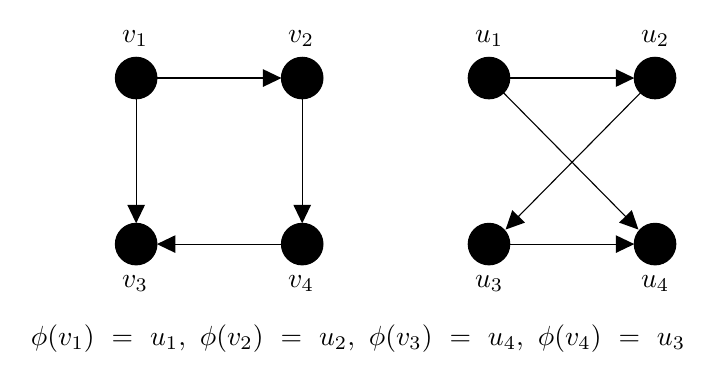
\begin{tikzpicture}[x=0.75pt,y=0.75pt,yscale=-1,xscale=1]
%uncomment if require: \path (0,184); %set diagram left start at 0, and has height of 184

%Straight Lines [id:da028261783525769912] 
\draw    (80,40) -- (137,40) ;
\draw [shift={(140,40)}, rotate = 180] [fill={rgb, 255:red, 0; green, 0; blue, 0 }  ][line width=0.08]  [draw opacity=0] (8.93,-4.29) -- (0,0) -- (8.93,4.29) -- cycle    ;
%Straight Lines [id:da5868154504079766] 
\draw    (70,50) -- (70,107) ;
\draw [shift={(70,110)}, rotate = 270] [fill={rgb, 255:red, 0; green, 0; blue, 0 }  ][line width=0.08]  [draw opacity=0] (8.93,-4.29) -- (0,0) -- (8.93,4.29) -- cycle    ;
%Straight Lines [id:da924843990160408] 
\draw    (150,50) -- (150,107) ;
\draw [shift={(150,110)}, rotate = 270] [fill={rgb, 255:red, 0; green, 0; blue, 0 }  ][line width=0.08]  [draw opacity=0] (8.93,-4.29) -- (0,0) -- (8.93,4.29) -- cycle    ;
%Straight Lines [id:da5222651223841381] 
\draw    (150,120) -- (83,120) ;
\draw [shift={(80,120)}, rotate = 360] [fill={rgb, 255:red, 0; green, 0; blue, 0 }  ][line width=0.08]  [draw opacity=0] (8.93,-4.29) -- (0,0) -- (8.93,4.29) -- cycle    ;
%Straight Lines [id:da35800782746944226] 
\draw    (240,40) -- (307,40) ;
\draw [shift={(310,40)}, rotate = 180] [fill={rgb, 255:red, 0; green, 0; blue, 0 }  ][line width=0.08]  [draw opacity=0] (8.93,-4.29) -- (0,0) -- (8.93,4.29) -- cycle    ;
%Straight Lines [id:da8484709903750047] 
\draw    (320,40) -- (250.11,110.86) ;
\draw [shift={(248,113)}, rotate = 314.6] [fill={rgb, 255:red, 0; green, 0; blue, 0 }  ][line width=0.08]  [draw opacity=0] (8.93,-4.29) -- (0,0) -- (8.93,4.29) -- cycle    ;
%Straight Lines [id:da4507216096132718] 
\draw    (240,120) -- (307,120) ;
\draw [shift={(310,120)}, rotate = 180] [fill={rgb, 255:red, 0; green, 0; blue, 0 }  ][line width=0.08]  [draw opacity=0] (8.93,-4.29) -- (0,0) -- (8.93,4.29) -- cycle    ;
%Shape: Circle [id:dp21486075935828408] 
\draw  [color={rgb, 255:red, 0; green, 0; blue, 0 }  ,draw opacity=1 ][fill={rgb, 255:red, 0; green, 0; blue, 0 }  ,fill opacity=1 ] (60,40) .. controls (60,34.48) and (64.48,30) .. (70,30) .. controls (75.52,30) and (80,34.48) .. (80,40) .. controls (80,45.52) and (75.52,50) .. (70,50) .. controls (64.48,50) and (60,45.52) .. (60,40) -- cycle ;
%Shape: Circle [id:dp6701725797486138] 
\draw  [color={rgb, 255:red, 0; green, 0; blue, 0 }  ,draw opacity=1 ][fill={rgb, 255:red, 0; green, 0; blue, 0 }  ,fill opacity=1 ] (140,40) .. controls (140,34.48) and (144.48,30) .. (150,30) .. controls (155.52,30) and (160,34.48) .. (160,40) .. controls (160,45.52) and (155.52,50) .. (150,50) .. controls (144.48,50) and (140,45.52) .. (140,40) -- cycle ;
%Shape: Circle [id:dp6472973243115998] 
\draw  [color={rgb, 255:red, 0; green, 0; blue, 0 }  ,draw opacity=1 ][fill={rgb, 255:red, 0; green, 0; blue, 0 }  ,fill opacity=1 ] (60,120) .. controls (60,114.48) and (64.48,110) .. (70,110) .. controls (75.52,110) and (80,114.48) .. (80,120) .. controls (80,125.52) and (75.52,130) .. (70,130) .. controls (64.48,130) and (60,125.52) .. (60,120) -- cycle ;
%Shape: Circle [id:dp7040441298715889] 
\draw  [color={rgb, 255:red, 0; green, 0; blue, 0 }  ,draw opacity=1 ][fill={rgb, 255:red, 0; green, 0; blue, 0 }  ,fill opacity=1 ] (140,120) .. controls (140,114.48) and (144.48,110) .. (150,110) .. controls (155.52,110) and (160,114.48) .. (160,120) .. controls (160,125.52) and (155.52,130) .. (150,130) .. controls (144.48,130) and (140,125.52) .. (140,120) -- cycle ;
%Shape: Circle [id:dp10694591732919978] 
\draw  [color={rgb, 255:red, 0; green, 0; blue, 0 }  ,draw opacity=1 ][fill={rgb, 255:red, 0; green, 0; blue, 0 }  ,fill opacity=1 ] (230,40) .. controls (230,34.48) and (234.48,30) .. (240,30) .. controls (245.52,30) and (250,34.48) .. (250,40) .. controls (250,45.52) and (245.52,50) .. (240,50) .. controls (234.48,50) and (230,45.52) .. (230,40) -- cycle ;
%Shape: Circle [id:dp7474241474824288] 
\draw  [color={rgb, 255:red, 0; green, 0; blue, 0 }  ,draw opacity=1 ][fill={rgb, 255:red, 0; green, 0; blue, 0 }  ,fill opacity=1 ] (310,40) .. controls (310,34.48) and (314.48,30) .. (320,30) .. controls (325.52,30) and (330,34.48) .. (330,40) .. controls (330,45.52) and (325.52,50) .. (320,50) .. controls (314.48,50) and (310,45.52) .. (310,40) -- cycle ;
%Shape: Circle [id:dp9814761785009831] 
\draw  [color={rgb, 255:red, 0; green, 0; blue, 0 }  ,draw opacity=1 ][fill={rgb, 255:red, 0; green, 0; blue, 0 }  ,fill opacity=1 ] (230,120) .. controls (230,114.48) and (234.48,110) .. (240,110) .. controls (245.52,110) and (250,114.48) .. (250,120) .. controls (250,125.52) and (245.52,130) .. (240,130) .. controls (234.48,130) and (230,125.52) .. (230,120) -- cycle ;
%Shape: Circle [id:dp0886867235763964] 
\draw  [color={rgb, 255:red, 0; green, 0; blue, 0 }  ,draw opacity=1 ][fill={rgb, 255:red, 0; green, 0; blue, 0 }  ,fill opacity=1 ] (310,120) .. controls (310,114.48) and (314.48,110) .. (320,110) .. controls (325.52,110) and (330,114.48) .. (330,120) .. controls (330,125.52) and (325.52,130) .. (320,130) .. controls (314.48,130) and (310,125.52) .. (310,120) -- cycle ;
%Straight Lines [id:da09396840754522406] 
\draw    (240,40) -- (309.89,110.86) ;
\draw [shift={(312,113)}, rotate = 225.4] [fill={rgb, 255:red, 0; green, 0; blue, 0 }  ][line width=0.08]  [draw opacity=0] (8.93,-4.29) -- (0,0) -- (8.93,4.29) -- cycle    ;

% Text Node
\draw (62,16) node [anchor=north west][inner sep=0.75pt]    {$v_{1}$};
% Text Node
\draw (142,16) node [anchor=north west][inner sep=0.75pt]    {$v_{2}$};
% Text Node
\draw (142,134) node [anchor=north west][inner sep=0.75pt]    {$v_{4}$};
% Text Node
\draw (62,134) node [anchor=north west][inner sep=0.75pt]    {$v_{3}$};
% Text Node
\draw (232,16) node [anchor=north west][inner sep=0.75pt]    {$u_{1}$};
% Text Node
\draw (312,16) node [anchor=north west][inner sep=0.75pt]    {$u_{2}$};
% Text Node
\draw (312,134) node [anchor=north west][inner sep=0.75pt]    {$u_{4}$};
% Text Node
\draw (232,134) node [anchor=north west][inner sep=0.75pt]    {$u_{3}$};
% Text Node
\draw (18,157.4) node [anchor=north west][inner sep=0.75pt]    {$\phi ( v_{1}) \ =\ u_{1} ,\ \phi ( v_{2}) \ =\ u_{2} ,\ \phi ( v_{3}) \ =\ u_{4} ,\ \phi ( v_{4}) \ =\ u_{3}$};


\end{tikzpicture}}
        \caption{Isomorphism.}
        \label{fig:isomorphism}
    \end{subfigure}
    \begin{subfigure}[b]{0.48\linewidth}
        \centering
        \resizebox{.9\textwidth}{!}{

\tikzset{every picture/.style={line width=0.75pt}} %set default line width to 0.75pt        

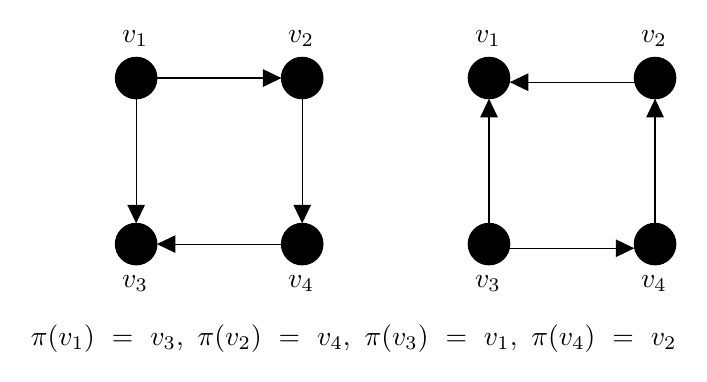
\begin{tikzpicture}[x=0.75pt,y=0.75pt,yscale=-1,xscale=1]
%uncomment if require: \path (0,194); %set diagram left start at 0, and has height of 194

%Straight Lines [id:da2955392181495553] 
\draw    (80,40) -- (137,40) ;
\draw [shift={(140,40)}, rotate = 180] [fill={rgb, 255:red, 0; green, 0; blue, 0 }  ][line width=0.08]  [draw opacity=0] (8.93,-4.29) -- (0,0) -- (8.93,4.29) -- cycle    ;
%Straight Lines [id:da5305038967662998] 
\draw    (70,50) -- (70,107) ;
\draw [shift={(70,110)}, rotate = 270] [fill={rgb, 255:red, 0; green, 0; blue, 0 }  ][line width=0.08]  [draw opacity=0] (8.93,-4.29) -- (0,0) -- (8.93,4.29) -- cycle    ;
%Straight Lines [id:da504741823915166] 
\draw    (150,50) -- (150,107) ;
\draw [shift={(150,110)}, rotate = 270] [fill={rgb, 255:red, 0; green, 0; blue, 0 }  ][line width=0.08]  [draw opacity=0] (8.93,-4.29) -- (0,0) -- (8.93,4.29) -- cycle    ;
%Straight Lines [id:da679331263093423] 
\draw    (140,120) -- (83,120) ;
\draw [shift={(80,120)}, rotate = 360] [fill={rgb, 255:red, 0; green, 0; blue, 0 }  ][line width=0.08]  [draw opacity=0] (8.93,-4.29) -- (0,0) -- (8.93,4.29) -- cycle    ;
%Straight Lines [id:da4417681262418318] 
\draw    (250,122) -- (307,122) ;
\draw [shift={(310,122)}, rotate = 180] [fill={rgb, 255:red, 0; green, 0; blue, 0 }  ][line width=0.08]  [draw opacity=0] (8.93,-4.29) -- (0,0) -- (8.93,4.29) -- cycle    ;
%Straight Lines [id:da2566742594564193] 
\draw    (240,110) -- (240,53) ;
\draw [shift={(240,50)}, rotate = 450] [fill={rgb, 255:red, 0; green, 0; blue, 0 }  ][line width=0.08]  [draw opacity=0] (8.93,-4.29) -- (0,0) -- (8.93,4.29) -- cycle    ;
%Straight Lines [id:da0962553210683279] 
\draw    (320,112) -- (320,53) ;
\draw [shift={(320,50)}, rotate = 450] [fill={rgb, 255:red, 0; green, 0; blue, 0 }  ][line width=0.08]  [draw opacity=0] (8.93,-4.29) -- (0,0) -- (8.93,4.29) -- cycle    ;
%Straight Lines [id:da6650885284512231] 
\draw    (310,42) -- (253,42) ;
\draw [shift={(250,42)}, rotate = 360] [fill={rgb, 255:red, 0; green, 0; blue, 0 }  ][line width=0.08]  [draw opacity=0] (8.93,-4.29) -- (0,0) -- (8.93,4.29) -- cycle    ;
%Shape: Circle [id:dp6035520182128737] 
\draw  [color={rgb, 255:red, 0; green, 0; blue, 0 }  ,draw opacity=1 ][fill={rgb, 255:red, 0; green, 0; blue, 0 }  ,fill opacity=1 ] (60,40) .. controls (60,34.48) and (64.48,30) .. (70,30) .. controls (75.52,30) and (80,34.48) .. (80,40) .. controls (80,45.52) and (75.52,50) .. (70,50) .. controls (64.48,50) and (60,45.52) .. (60,40) -- cycle ;
%Shape: Circle [id:dp47334562116619106] 
\draw  [color={rgb, 255:red, 0; green, 0; blue, 0 }  ,draw opacity=1 ][fill={rgb, 255:red, 0; green, 0; blue, 0 }  ,fill opacity=1 ] (140,40) .. controls (140,34.48) and (144.48,30) .. (150,30) .. controls (155.52,30) and (160,34.48) .. (160,40) .. controls (160,45.52) and (155.52,50) .. (150,50) .. controls (144.48,50) and (140,45.52) .. (140,40) -- cycle ;
%Shape: Circle [id:dp06575432699841222] 
\draw  [color={rgb, 255:red, 0; green, 0; blue, 0 }  ,draw opacity=1 ][fill={rgb, 255:red, 0; green, 0; blue, 0 }  ,fill opacity=1 ] (140,120) .. controls (140,114.48) and (144.48,110) .. (150,110) .. controls (155.52,110) and (160,114.48) .. (160,120) .. controls (160,125.52) and (155.52,130) .. (150,130) .. controls (144.48,130) and (140,125.52) .. (140,120) -- cycle ;
%Shape: Circle [id:dp7218499293087284] 
\draw  [color={rgb, 255:red, 0; green, 0; blue, 0 }  ,draw opacity=1 ][fill={rgb, 255:red, 0; green, 0; blue, 0 }  ,fill opacity=1 ] (60,120) .. controls (60,114.48) and (64.48,110) .. (70,110) .. controls (75.52,110) and (80,114.48) .. (80,120) .. controls (80,125.52) and (75.52,130) .. (70,130) .. controls (64.48,130) and (60,125.52) .. (60,120) -- cycle ;
%Shape: Circle [id:dp5770118231708317] 
\draw  [color={rgb, 255:red, 0; green, 0; blue, 0 }  ,draw opacity=1 ][fill={rgb, 255:red, 0; green, 0; blue, 0 }  ,fill opacity=1 ] (230,40) .. controls (230,34.48) and (234.48,30) .. (240,30) .. controls (245.52,30) and (250,34.48) .. (250,40) .. controls (250,45.52) and (245.52,50) .. (240,50) .. controls (234.48,50) and (230,45.52) .. (230,40) -- cycle ;
%Shape: Circle [id:dp13036696544547421] 
\draw  [color={rgb, 255:red, 0; green, 0; blue, 0 }  ,draw opacity=1 ][fill={rgb, 255:red, 0; green, 0; blue, 0 }  ,fill opacity=1 ] (310,40) .. controls (310,34.48) and (314.48,30) .. (320,30) .. controls (325.52,30) and (330,34.48) .. (330,40) .. controls (330,45.52) and (325.52,50) .. (320,50) .. controls (314.48,50) and (310,45.52) .. (310,40) -- cycle ;
%Shape: Circle [id:dp6754342457309832] 
\draw  [color={rgb, 255:red, 0; green, 0; blue, 0 }  ,draw opacity=1 ][fill={rgb, 255:red, 0; green, 0; blue, 0 }  ,fill opacity=1 ] (310,120) .. controls (310,114.48) and (314.48,110) .. (320,110) .. controls (325.52,110) and (330,114.48) .. (330,120) .. controls (330,125.52) and (325.52,130) .. (320,130) .. controls (314.48,130) and (310,125.52) .. (310,120) -- cycle ;
%Shape: Circle [id:dp28508314737254614] 
\draw  [color={rgb, 255:red, 0; green, 0; blue, 0 }  ,draw opacity=1 ][fill={rgb, 255:red, 0; green, 0; blue, 0 }  ,fill opacity=1 ] (230,120) .. controls (230,114.48) and (234.48,110) .. (240,110) .. controls (245.52,110) and (250,114.48) .. (250,120) .. controls (250,125.52) and (245.52,130) .. (240,130) .. controls (234.48,130) and (230,125.52) .. (230,120) -- cycle ;

% Text Node
\draw (62,16) node [anchor=north west][inner sep=0.75pt]    {$v_{1}$};
% Text Node
\draw (142,16) node [anchor=north west][inner sep=0.75pt]    {$v_{2}$};
% Text Node
\draw (142,134) node [anchor=north west][inner sep=0.75pt]    {$v_{4}$};
% Text Node
\draw (62,134) node [anchor=north west][inner sep=0.75pt]    {$v_{3}$};
% Text Node
\draw (18,157.4) node [anchor=north west][inner sep=0.75pt]    {$\pi ( v_{1}) \ =\ v_{3} ,\ \pi ( v_{2}) \ =\ v_{4} ,\ \pi ( v_{3}) \ =\ v_{1} ,\ \pi ( v_{4}) \ =\ v_{2}$};
% Text Node
\draw (232,16) node [anchor=north west][inner sep=0.75pt]    {$v_{1}$};
% Text Node
\draw (312,16) node [anchor=north west][inner sep=0.75pt]    {$v_{2}$};
% Text Node
\draw (312,134) node [anchor=north west][inner sep=0.75pt]    {$v_{4}$};
% Text Node
\draw (232,134) node [anchor=north west][inner sep=0.75pt]    {$v_{3}$};


\end{tikzpicture}}
        \caption{Automorphism.}
        \label{fig:automorphism}
    \end{subfigure}
    \caption{An example of graph isomorphism and automorphism.}
\end{figure*}

\subsection{Graphs Matrices} \label{sec:adj-matrix}
One compact way to represent the structure of a graph is through its  \keyword{adjacency matrix}. Given a graph $\Graph{g}$ with $n$ vertices and $m$ edges, the entries $a_{ij}$ of its corresponding  adjacency matrix $\AdjMatrix{g} \in \Real^{n \times n}$ are defined as follows:
\[
a_{ij} =
    \begin{cases}
        1  & \text{if } (v_i, v_j) \in \Edges{g}\\
        0  & \text{otherwise.}
    \end{cases}
\]
Note that the diagonal entries $a_{ii}$ of the adjacency matrix specify the presence  (or absence) of self-loops. Another interesting property of the adjacency matrix is that  it is symmetric for undirected graphs, which implies $a_{ij} = a_{ji},$ $\forall\, i, j = 1, \ldots, n$. Adjacency matrices make some calculations of graph properties particularly convenient: for example, the in-degree and out-degree of a vertex $v_j \in \Nodes{g}$
can be obtained by performing row-wise and column-wise sums on $\AdjMatrix{g}$:
$$
\Fun{degree}_{out}(v_j) = \sum_{i=1}^n a_{ji} \quad \quad \Fun{degree}_{in}(v_j) = \sum_{i=1}^n a_{ij}.
$$
Adjacency matrices are also useful to understand concepts such as graph automorphism: in fact, an automorphism of $\Graph{g}$ corresponds to a permutation of the columns or rows of the adjacency matrix (but not both). Other useful matrices to represent properties of graphs are the \emph{Laplacian matrix} $\LaplacianMatrix{g} \in \Real^{n \times n} = \DegreeMatrix{g} - \AdjMatrix{g}$, and the \emph{symmetric normalized Laplacian matrix} $\NormLaplacianMatrix{g} \in \Real^{n \times n} = \Identity - \DegreeMatrix{g}^{-\frac{1}{2}}\AdjMatrix{g}\DegreeMatrix{g}^{-\frac{1}{2}}$. In both definitions, the matrix  $\DegreeMatrix{g} \in \Real^{n \times n}$ is the \emph{degree matrix}, where all entries are zero except the diagonal entries, for which $d_{ii} = \Fun{degree}(v_i)$. These matrices provide information about the graph connectivity through their eigenvalues and eigenvectors. Following, we shall use $\AdjMatrix{g}$ instead of $\Graph{g}$ to denote the structure of the graph whenever needed from the context.

\section{The Adaptive Processing of Structured Data}
The processing of structured data for learning purposes is carried out by a \keyword{structural transduction}, namely a function $\Transduction: \Cal{x} \shortrightarrow \Cal{y}$ where $\Cal{X}$ and $\Cal{Y}$ are structured domains. When the structural transduction is implemented by a (deep) \gls{nn}, it is \emph{adaptive}, \ie it is learned from data. A structural transduction can be decomposed as $\Transduction = \EncTrans \circ \OutTrans$, where:
\begin{itemize}
    \item $\EncTrans$ is called \emph{encoding function} or \emph{state transition function}, and it is applied separately to each element of the structure. The output of the encoding function is a structure isomorphic to that in input, where the elements are now \keyword{state vectors}. Intuitively, a state vector encodes the information of its corresponding element and of the elements it depends on;
    \item $\OutTrans$ is called \emph{output function}, which computes an output from the state vectors.
\end{itemize}
The output function of the structural transduction is task-dependent. Considering a supervised setting and a generic graph dataset $\Data$ consisting of $n$ training pairs, we distinguish two learning problems:
\begin{itemize}
    \item in \emph{structure-to-structure} tasks, the dataset is composed of pairs of attributed graphs $\Data = \{(\PatternGraph{g}{i}, \PatternGraph{h}{i})\}_{i=1}^n$, where $\AttrGraph{g} = \VectorGraph{x}{g}$ is an input graph, $\AttrGraph{h} = \VectorGraph{y}{h}$ is an output graph, and the two underlying unattributed graphs $\Graph{g}$ and $\Graph{h}$ are isomorphic under a bijection $\vartheta$. The task is to predict the target associated to an output graph vertex, given the corresponding features of its isomorphic vertex. The objective function minimized in these tasks is the following:
    $$\argmin_{\Param} \frac{1}{n} \sum_{i=1}^n -\log p(\PatternGraph{h}{i} \given \PatternGraph{g}{i}) = -\frac{1}{n} \sum_{i=1}^n \sum_{v \in \Nodes{g_{(i)}}} -\log p(\Elem{y}{\vartheta(v)} \given \Elem{x}{v});$$
    \item in \emph{structure-to-element} tasks, the dataset has the form  $\Data = \{(\PatternGraph{g}{i}, \PatternVector{y}{i})\}_{i=1}^n$, where $\AttrGraph{g} = \VectorGraph{x}{g}$ is an input graph and $\Vector{y} \in \Real^y$ is an output vector. The task is to predict a single output vector (or scalar) from the structure and the features of $\AttrGraph{g}$. The  objective function minimized in these tasks is the following:
    $$\argmin_{\Param} \frac{1}{n} \sum_{i=1}^n - \log p(\PatternVector{y}{i} \given \PatternGraph{g}{i}).$$
    To learn structure-to-element tasks, the output function must compress the states of each element of the structure into a global output vector representing the entire structure, which is compared to the target $\Vector{y}$. To do so, there are several strategies; in general, one could pick a single state vector as a representative for the whole structure, or compute a summary of the entire structure using all the available state vectors. The function that implements the latter strategy is usually termed \keyword{readout}.
\end{itemize}

As anticipated, one important issue that structural transductions need to address is how to deal with variable-sized inputs. The solution is to apply the same state transition function (that is, with the same adaptive parameters) \emph{locally} to every element in the structure, rather than to the overall structure. This process is similar to the localized processing of images performed by \glspl{cnn}, which work by considering a single pixel at a time, and combining it with some finite set of nearby pixels. This local property of the structural transduction is often referred to as \emph{stationarity}. An interesting byproduct of using stationary transductions is that they require a smaller number of parameters with respect to non-stationary ones, since the network weights are shared across the structure. At the same time, using stationary transductions also requires additional mechanisms to learn from the global structure of the datum (such as readouts in the case of structure-to-element tasks), rather than only locally.

In the following sections, we present three specific \gls{nn} architectures that implement transductions over structured data: recurrent neural networks, which process data represented as sequences; recursive neural networks, which process hierarchical data such as trees; and deep graph networks, which process general graphs.

\section{Recurrent Neural Networks}\label{sec:rnns}
A \gls{rnn} is a \gls{nn} architecture able to process sequences. Let $\AttrGraph{S}$ be an attributed sequence of length $m$ with elements $\Nodes{s} = (v_1, v_2, \ldots, v_m)$, and let $\GraphFeatures{x}{s} = \Par{\Elem{x}{1}, \Elem{x}{2}, \ldots, \Elem{x}{m}}$ be its element features. Here, we slightly abuse the notation $\Elem{x}{v_t}$ in favor of $\Elem{x}{t}$, since sequence elements are ordered. Let us assume a supervised setting, and the availability of an isomorphic attributed sequence $\AttrGraph{R}$ with targets $\GraphFeatures{y}{r} = \Par{\Elem{y}{1}, \Elem{y}{2}, \ldots, \Elem{y}{m}}$. The state transition function of a \gls{rnn}, applied locally to each sequence element, has the following general form:
\begin{align*}
    \Elem{h}{t} =
    \begin{cases}
        \boldsymbol{0} & \mathrm{if}\; t = 0\\
        \EncTrans(\Elem{x}{t}, \Elem{h}{t-1}) & \mathrm{otherwise},
    \end{cases}
\end{align*}
where $\Elem{h}{t} \in \Real^h$ is a state vector, also known as \keyword{hidden state}, and $\boldsymbol{0}$ is a zero vector. The calculation of the hidden state performed by the state transition function $\EncTrans$ is \emph{recursive}: to compute a hidden state for the $t$-th element of the sequence, the hidden state of the previous element must be known in advance. Thus, the state computation is a sequential process, where the input sequence is traversed in order one element at a time, and the hidden state is updated as a function of the current sequence element and the hidden state at the previous step. To avoid infinite recursion, the hidden state is initialized with the zero vector $\Elem{h}{0} = \boldsymbol{0}$. As the sequence is traversed, the hidden state maintains a \emph{memory} of the past elements of the sequence. The presence of a memory mechanism makes \glspl{rnn} very powerful: in fact, it has been proved that finite-size \glspl{rnn} can compute any function computable with a Turing machine \citep{siegelmann1995rnnturing}. As with \glspl{cnn}, the development of \glspl{rnn} started in the early '90s, and they have recently been rediscovered within the \gls{dl} framework after their success, especially in \gls{nlp}-related tasks.

\subsection{Training}
Given an attributed sequence $\Seq{S}$ with features $\Vector{x}_{\Seq{s}}$, the original implementation of the state transition function of a \gls{rnn} is defined as follows\footnote{For the rest of this chapter, biases are omitted for readability.}:
\begin{align*}
    \Elem{h}{t} &= \tanh\Par{\Matrix{W}\Elem{x}{t} + \Matrix{U}\Elem{h}{t-1}},\; \forall t=1, \ldots, m.
\end{align*}
The above is also called \keyword{recurrent layer}. The weight matrices $\Matrix{W} \in \Real^{d \times h}$ and $\Matrix{U} \in \Real^{h \times h}$, are shared among the sequence elements according to the stationarity property. For this reason, it is often said that the network is \emph{unrolled} over the sequence. In structure-to-structure tasks, once the states of the elements are calculated, an element-wise output is computed as:
\begin{align*}
    \Elem{o}{t} = g(\Elem{h}{t}),\; \forall t=1, \ldots, m,
\end{align*}
where $g$ can be any neural network such as one simple output layer or a more complex downstream network. Similarly, in structure-to-element tasks, a single output is computed from the last hidden state of the sequence:
\begin{align*}
    \Vector{o} = g(\Elem{h}{m}).
\end{align*}
Figure \ref{fig:rnn-unfold} shows a \gls{rnn} in compact form, as well as unrolled over a sequence of length $m$ for a structure-to-structure task. The error of the network during training is computed by comparing the output of the network for each sequence element $\Elem{o}{t}$ to the isomorphic sequence element $\Elem{y}{t}$ in the target sequence with the loss function $\Loss$. The loss is summed up over all the elements in the sequence, and averaged over all sequences in the dataset to minimize the \gls{mle} objective. Notice that it is possible to stack multiple recurrent layers and create deep \glspl{rnn} by feeding the hidden state produced by a recurrent layer as input to a subsequent recurrent layer, other than to the next step of the recurrence. In these cases, the output is computed after by the last recurrent layer in the stack.
\begin{figure*}[h!]
    \begin{subfigure}[b]{0.39\linewidth}
        \centering
        \resizebox{.7\textwidth}{!}{

\tikzset{every picture/.style={line width=0.75pt}} %set default line width to 0.75pt

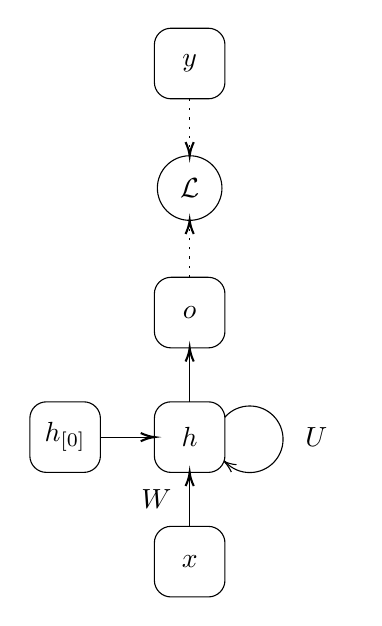
\begin{tikzpicture}[x=0.75pt,y=0.75pt,yscale=-1,xscale=1]
%uncomment if require: \path (0,300); %set diagram left start at 0, and has height of 300

%Shape: Circle [id:dp23367042930106008]
\draw   (107.92,216.04) .. controls (107.92,207.18) and (115.1,200) .. (123.96,200) .. controls (132.82,200) and (140,207.18) .. (140,216.04) .. controls (140,224.9) and (132.82,232.08) .. (123.96,232.08) .. controls (115.1,232.08) and (107.92,224.9) .. (107.92,216.04) -- cycle ;
\draw   (115.05,231.82) .. controls (114.1,229.66) and (112.86,227.9) .. (111.36,226.53) .. controls (113.14,227.51) and (115.22,228.09) .. (117.57,228.29) ;

% Text Node
\draw    (78,266) .. controls (78,261.58) and (81.58,258) .. (86,258) -- (104,258) .. controls (108.42,258) and (112,261.58) .. (112,266) -- (112,284) .. controls (112,288.42) and (108.42,292) .. (104,292) -- (86,292) .. controls (81.58,292) and (78,288.42) .. (78,284) -- cycle  ;
\draw (95,275) node   [align=left] {\begin{minipage}[lt]{20.400000000000002pt}\setlength\topsep{0pt}
\begin{center}
$\displaystyle \boldsymbol{x}$
\end{center}

\end{minipage}};
% Text Node
\draw  [fill={rgb, 255:red, 255; green, 255; blue, 255 }  ,fill opacity=1 ]  (78,206) .. controls (78,201.58) and (81.58,198) .. (86,198) -- (104,198) .. controls (108.42,198) and (112,201.58) .. (112,206) -- (112,224) .. controls (112,228.42) and (108.42,232) .. (104,232) -- (86,232) .. controls (81.58,232) and (78,228.42) .. (78,224) -- cycle  ;
\draw (95,215) node   [align=left] {\begin{minipage}[lt]{20.400000000000002pt}\setlength\topsep{0pt}
\begin{center}
$\displaystyle \boldsymbol{h}$
\end{center}

\end{minipage}};
% Text Node
\draw    (18,206) .. controls (18,201.58) and (21.58,198) .. (26,198) -- (44,198) .. controls (48.42,198) and (52,201.58) .. (52,206) -- (52,224) .. controls (52,228.42) and (48.42,232) .. (44,232) -- (26,232) .. controls (21.58,232) and (18,228.42) .. (18,224) -- cycle  ;
\draw (35,215) node   [align=left] {\begin{minipage}[lt]{20.400000000000002pt}\setlength\topsep{0pt}
\begin{center}
$\displaystyle \boldsymbol{h}_{[ 0]}$
\end{center}

\end{minipage}};
% Text Node
\draw    (78,146) .. controls (78,141.58) and (81.58,138) .. (86,138) -- (104,138) .. controls (108.42,138) and (112,141.58) .. (112,146) -- (112,164) .. controls (112,168.42) and (108.42,172) .. (104,172) -- (86,172) .. controls (81.58,172) and (78,168.42) .. (78,164) -- cycle  ;
\draw (95,155) node   [align=left] {\begin{minipage}[lt]{20.400000000000002pt}\setlength\topsep{0pt}
\begin{center}
$\displaystyle \boldsymbol{o}$
\end{center}

\end{minipage}};
% Text Node
\draw    (78,26) .. controls (78,21.58) and (81.58,18) .. (86,18) -- (104,18) .. controls (108.42,18) and (112,21.58) .. (112,26) -- (112,44) .. controls (112,48.42) and (108.42,52) .. (104,52) -- (86,52) .. controls (81.58,52) and (78,48.42) .. (78,44) -- cycle  ;
\draw (95,35) node   [align=left] {\begin{minipage}[lt]{20.400000000000002pt}\setlength\topsep{0pt}
\begin{center}
$\displaystyle \boldsymbol{y}$
\end{center}

\end{minipage}};
% Text Node
\draw (156,215) node   [align=left] {\begin{minipage}[lt]{20.400000000000002pt}\setlength\topsep{0pt}
\begin{center}
$\displaystyle \boldsymbol{U}$
\end{center}

\end{minipage}};
% Text Node
\draw (79,245) node   [align=left] {\begin{minipage}[lt]{20.400000000000002pt}\setlength\topsep{0pt}
\begin{center}
$\displaystyle \boldsymbol{W}$
\end{center}

\end{minipage}};
% Text Node
\draw    (95, 95) circle [x radius= 15.56, y radius= 15.56]   ;
\draw (95,95) node   [align=left] {\begin{minipage}[lt]{13.735995849609345pt}\setlength\topsep{0pt}
\begin{center}
$\displaystyle \mathcal{L}$
\end{center}

\end{minipage}};
% Connection
\draw    (95,258) -- (95,234) ;
\draw [shift={(95,232)}, rotate = 450] [color={rgb, 255:red, 0; green, 0; blue, 0 }  ][line width=0.75]    (6.56,-1.97) .. controls (4.17,-0.84) and (1.99,-0.18) .. (0,0) .. controls (1.99,0.18) and (4.17,0.84) .. (6.56,1.97)   ;
% Connection
\draw    (52,215) -- (76,215) ;
\draw [shift={(78,215)}, rotate = 180] [color={rgb, 255:red, 0; green, 0; blue, 0 }  ][line width=0.75]    (6.56,-1.97) .. controls (4.17,-0.84) and (1.99,-0.18) .. (0,0) .. controls (1.99,0.18) and (4.17,0.84) .. (6.56,1.97)   ;
% Connection
\draw    (95,198) -- (95,174) ;
\draw [shift={(95,172)}, rotate = 450] [color={rgb, 255:red, 0; green, 0; blue, 0 }  ][line width=0.75]    (6.56,-1.97) .. controls (4.17,-0.84) and (1.99,-0.18) .. (0,0) .. controls (1.99,0.18) and (4.17,0.84) .. (6.56,1.97)   ;
% Connection
\draw  [dash pattern={on 0.84pt off 2.51pt}]  (95,138) -- (95,112.56) ;
\draw [shift={(95,110.56)}, rotate = 450] [color={rgb, 255:red, 0; green, 0; blue, 0 }  ][line width=0.75]    (6.56,-1.97) .. controls (4.17,-0.84) and (1.99,-0.18) .. (0,0) .. controls (1.99,0.18) and (4.17,0.84) .. (6.56,1.97)   ;
% Connection
\draw  [dash pattern={on 0.84pt off 2.51pt}]  (95,52) -- (95,77.44) ;
\draw [shift={(95,79.44)}, rotate = 270] [color={rgb, 255:red, 0; green, 0; blue, 0 }  ][line width=0.75]    (6.56,-1.97) .. controls (4.17,-0.84) and (1.99,-0.18) .. (0,0) .. controls (1.99,0.18) and (4.17,0.84) .. (6.56,1.97)   ;

\end{tikzpicture}}
        \caption{}
        \label{fig:rnn}
    \end{subfigure}
    \begin{subfigure}[b]{0.59\linewidth}
        \centering
        \resizebox{.8\textwidth}{!}{

\tikzset{every picture/.style={line width=0.75pt}} %set default line width to 0.75pt        

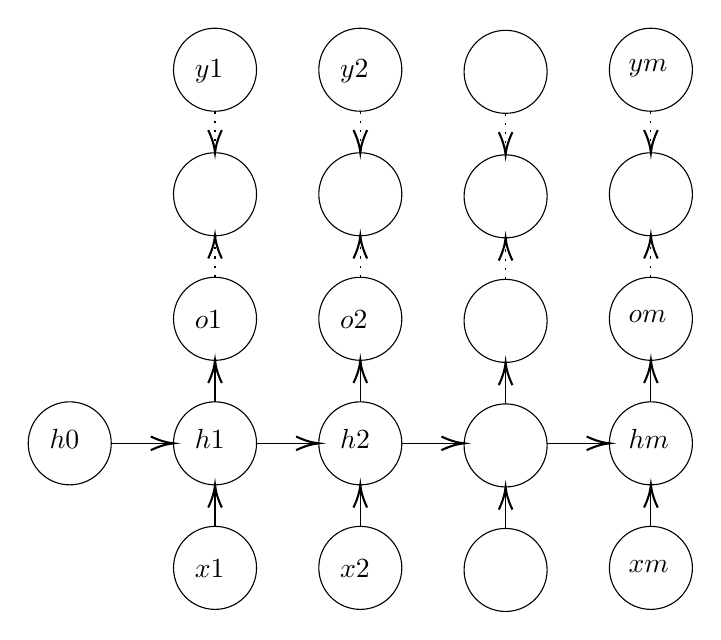
\begin{tikzpicture}[x=0.75pt,y=0.75pt,yscale=-1,xscale=1]
%uncomment if require: \path (0,323); %set diagram left start at 0, and has height of 323

%Shape: Circle [id:dp3629561388056113] 
\draw   (90,150) .. controls (90,138.95) and (98.95,130) .. (110,130) .. controls (121.05,130) and (130,138.95) .. (130,150) .. controls (130,161.05) and (121.05,170) .. (110,170) .. controls (98.95,170) and (90,161.05) .. (90,150) -- cycle ;
%Shape: Circle [id:dp44819185014685403] 
\draw   (160,150) .. controls (160,138.95) and (168.95,130) .. (180,130) .. controls (191.05,130) and (200,138.95) .. (200,150) .. controls (200,161.05) and (191.05,170) .. (180,170) .. controls (168.95,170) and (160,161.05) .. (160,150) -- cycle ;
%Shape: Circle [id:dp4778230592944719] 
\draw   (300,150) .. controls (300,138.95) and (308.95,130) .. (320,130) .. controls (331.05,130) and (340,138.95) .. (340,150) .. controls (340,161.05) and (331.05,170) .. (320,170) .. controls (308.95,170) and (300,161.05) .. (300,150) -- cycle ;
%Shape: Circle [id:dp4172940080920504] 
\draw   (90,210) .. controls (90,198.95) and (98.95,190) .. (110,190) .. controls (121.05,190) and (130,198.95) .. (130,210) .. controls (130,221.05) and (121.05,230) .. (110,230) .. controls (98.95,230) and (90,221.05) .. (90,210) -- cycle ;
%Shape: Circle [id:dp9221856908591408] 
\draw   (160,210) .. controls (160,198.95) and (168.95,190) .. (180,190) .. controls (191.05,190) and (200,198.95) .. (200,210) .. controls (200,221.05) and (191.05,230) .. (180,230) .. controls (168.95,230) and (160,221.05) .. (160,210) -- cycle ;
%Shape: Circle [id:dp5107698459287944] 
\draw   (300,210) .. controls (300,198.95) and (308.95,190) .. (320,190) .. controls (331.05,190) and (340,198.95) .. (340,210) .. controls (340,221.05) and (331.05,230) .. (320,230) .. controls (308.95,230) and (300,221.05) .. (300,210) -- cycle ;
%Shape: Circle [id:dp9971969777197274] 
\draw   (90,270) .. controls (90,258.95) and (98.95,250) .. (110,250) .. controls (121.05,250) and (130,258.95) .. (130,270) .. controls (130,281.05) and (121.05,290) .. (110,290) .. controls (98.95,290) and (90,281.05) .. (90,270) -- cycle ;
%Shape: Circle [id:dp6035985742831749] 
\draw   (160,270) .. controls (160,258.95) and (168.95,250) .. (180,250) .. controls (191.05,250) and (200,258.95) .. (200,270) .. controls (200,281.05) and (191.05,290) .. (180,290) .. controls (168.95,290) and (160,281.05) .. (160,270) -- cycle ;
%Shape: Circle [id:dp20977751188714566] 
\draw   (300,270) .. controls (300,258.95) and (308.95,250) .. (320,250) .. controls (331.05,250) and (340,258.95) .. (340,270) .. controls (340,281.05) and (331.05,290) .. (320,290) .. controls (308.95,290) and (300,281.05) .. (300,270) -- cycle ;
%Shape: Circle [id:dp23609841012892163] 
\draw   (90,30) .. controls (90,18.95) and (98.95,10) .. (110,10) .. controls (121.05,10) and (130,18.95) .. (130,30) .. controls (130,41.05) and (121.05,50) .. (110,50) .. controls (98.95,50) and (90,41.05) .. (90,30) -- cycle ;
%Shape: Circle [id:dp5318607092141312] 
\draw   (160,30) .. controls (160,18.95) and (168.95,10) .. (180,10) .. controls (191.05,10) and (200,18.95) .. (200,30) .. controls (200,41.05) and (191.05,50) .. (180,50) .. controls (168.95,50) and (160,41.05) .. (160,30) -- cycle ;
%Shape: Circle [id:dp7028223312018156] 
\draw   (300,30) .. controls (300,18.95) and (308.95,10) .. (320,10) .. controls (331.05,10) and (340,18.95) .. (340,30) .. controls (340,41.05) and (331.05,50) .. (320,50) .. controls (308.95,50) and (300,41.05) .. (300,30) -- cycle ;
%Shape: Circle [id:dp42488579033193763] 
\draw   (90,90) .. controls (90,78.95) and (98.95,70) .. (110,70) .. controls (121.05,70) and (130,78.95) .. (130,90) .. controls (130,101.05) and (121.05,110) .. (110,110) .. controls (98.95,110) and (90,101.05) .. (90,90) -- cycle ;
%Shape: Circle [id:dp1754771414071341] 
\draw   (160,90) .. controls (160,78.95) and (168.95,70) .. (180,70) .. controls (191.05,70) and (200,78.95) .. (200,90) .. controls (200,101.05) and (191.05,110) .. (180,110) .. controls (168.95,110) and (160,101.05) .. (160,90) -- cycle ;
%Shape: Circle [id:dp8997928679194878] 
\draw   (300,90) .. controls (300,78.95) and (308.95,70) .. (320,70) .. controls (331.05,70) and (340,78.95) .. (340,90) .. controls (340,101.05) and (331.05,110) .. (320,110) .. controls (308.95,110) and (300,101.05) .. (300,90) -- cycle ;
%Straight Lines [id:da8537414640186041] 
\draw    (110,250) -- (110,232) ;
\draw [shift={(110,230)}, rotate = 450] [color={rgb, 255:red, 0; green, 0; blue, 0 }  ][line width=0.75]    (10.93,-3.29) .. controls (6.95,-1.4) and (3.31,-0.3) .. (0,0) .. controls (3.31,0.3) and (6.95,1.4) .. (10.93,3.29)   ;
%Straight Lines [id:da8728240272525218] 
\draw    (180,250) -- (180,232) ;
\draw [shift={(180,230)}, rotate = 450] [color={rgb, 255:red, 0; green, 0; blue, 0 }  ][line width=0.75]    (10.93,-3.29) .. controls (6.95,-1.4) and (3.31,-0.3) .. (0,0) .. controls (3.31,0.3) and (6.95,1.4) .. (10.93,3.29)   ;
%Straight Lines [id:da3702106006623287] 
\draw    (320,250) -- (320,232) ;
\draw [shift={(320,230)}, rotate = 450] [color={rgb, 255:red, 0; green, 0; blue, 0 }  ][line width=0.75]    (10.93,-3.29) .. controls (6.95,-1.4) and (3.31,-0.3) .. (0,0) .. controls (3.31,0.3) and (6.95,1.4) .. (10.93,3.29)   ;
%Straight Lines [id:da8147113194897551] 
\draw    (110,190) -- (110,172) ;
\draw [shift={(110,170)}, rotate = 450] [color={rgb, 255:red, 0; green, 0; blue, 0 }  ][line width=0.75]    (10.93,-3.29) .. controls (6.95,-1.4) and (3.31,-0.3) .. (0,0) .. controls (3.31,0.3) and (6.95,1.4) .. (10.93,3.29)   ;
%Straight Lines [id:da9940060129323278] 
\draw    (180,190) -- (180,172) ;
\draw [shift={(180,170)}, rotate = 450] [color={rgb, 255:red, 0; green, 0; blue, 0 }  ][line width=0.75]    (10.93,-3.29) .. controls (6.95,-1.4) and (3.31,-0.3) .. (0,0) .. controls (3.31,0.3) and (6.95,1.4) .. (10.93,3.29)   ;
%Straight Lines [id:da21234167773916912] 
\draw    (320,190) -- (320,172) ;
\draw [shift={(320,170)}, rotate = 450] [color={rgb, 255:red, 0; green, 0; blue, 0 }  ][line width=0.75]    (10.93,-3.29) .. controls (6.95,-1.4) and (3.31,-0.3) .. (0,0) .. controls (3.31,0.3) and (6.95,1.4) .. (10.93,3.29)   ;
%Straight Lines [id:da51949842029655] 
\draw  [dash pattern={on 0.84pt off 2.51pt}]  (110,130) -- (110,112) ;
\draw [shift={(110,110)}, rotate = 450] [color={rgb, 255:red, 0; green, 0; blue, 0 }  ][line width=0.75]    (10.93,-3.29) .. controls (6.95,-1.4) and (3.31,-0.3) .. (0,0) .. controls (3.31,0.3) and (6.95,1.4) .. (10.93,3.29)   ;
%Straight Lines [id:da6212732550300433] 
\draw  [dash pattern={on 0.84pt off 2.51pt}]  (180,130) -- (180,112) ;
\draw [shift={(180,110)}, rotate = 450] [color={rgb, 255:red, 0; green, 0; blue, 0 }  ][line width=0.75]    (10.93,-3.29) .. controls (6.95,-1.4) and (3.31,-0.3) .. (0,0) .. controls (3.31,0.3) and (6.95,1.4) .. (10.93,3.29)   ;
%Straight Lines [id:da5634341890894232] 
\draw  [dash pattern={on 0.84pt off 2.51pt}]  (320,130) -- (320,112) ;
\draw [shift={(320,110)}, rotate = 450] [color={rgb, 255:red, 0; green, 0; blue, 0 }  ][line width=0.75]    (10.93,-3.29) .. controls (6.95,-1.4) and (3.31,-0.3) .. (0,0) .. controls (3.31,0.3) and (6.95,1.4) .. (10.93,3.29)   ;
%Straight Lines [id:da7517812400746318] 
\draw  [dash pattern={on 0.84pt off 2.51pt}]  (110,50) -- (110,68) ;
\draw [shift={(110,70)}, rotate = 270] [color={rgb, 255:red, 0; green, 0; blue, 0 }  ][line width=0.75]    (10.93,-3.29) .. controls (6.95,-1.4) and (3.31,-0.3) .. (0,0) .. controls (3.31,0.3) and (6.95,1.4) .. (10.93,3.29)   ;
%Straight Lines [id:da23656264229534862] 
\draw  [dash pattern={on 0.84pt off 2.51pt}]  (180,50) -- (180,68) ;
\draw [shift={(180,70)}, rotate = 270] [color={rgb, 255:red, 0; green, 0; blue, 0 }  ][line width=0.75]    (10.93,-3.29) .. controls (6.95,-1.4) and (3.31,-0.3) .. (0,0) .. controls (3.31,0.3) and (6.95,1.4) .. (10.93,3.29)   ;
%Straight Lines [id:da2050152758610957] 
\draw  [dash pattern={on 0.84pt off 2.51pt}]  (320,50) -- (320,68) ;
\draw [shift={(320,70)}, rotate = 270] [color={rgb, 255:red, 0; green, 0; blue, 0 }  ][line width=0.75]    (10.93,-3.29) .. controls (6.95,-1.4) and (3.31,-0.3) .. (0,0) .. controls (3.31,0.3) and (6.95,1.4) .. (10.93,3.29)   ;
%Straight Lines [id:da15141952791941238] 
\draw    (130,210) -- (158,210) ;
\draw [shift={(160,210)}, rotate = 180] [color={rgb, 255:red, 0; green, 0; blue, 0 }  ][line width=0.75]    (10.93,-3.29) .. controls (6.95,-1.4) and (3.31,-0.3) .. (0,0) .. controls (3.31,0.3) and (6.95,1.4) .. (10.93,3.29)   ;
%Straight Lines [id:da8773526556001805] 
\draw    (270,210) -- (298,210) ;
\draw [shift={(300,210)}, rotate = 180] [color={rgb, 255:red, 0; green, 0; blue, 0 }  ][line width=0.75]    (10.93,-3.29) .. controls (6.95,-1.4) and (3.31,-0.3) .. (0,0) .. controls (3.31,0.3) and (6.95,1.4) .. (10.93,3.29)   ;
%Shape: Circle [id:dp46244560624869613] 
\draw   (20,210) .. controls (20,198.95) and (28.95,190) .. (40,190) .. controls (51.05,190) and (60,198.95) .. (60,210) .. controls (60,221.05) and (51.05,230) .. (40,230) .. controls (28.95,230) and (20,221.05) .. (20,210) -- cycle ;
%Straight Lines [id:da797513658170024] 
\draw    (60,210) -- (88,210) ;
\draw [shift={(90,210)}, rotate = 180] [color={rgb, 255:red, 0; green, 0; blue, 0 }  ][line width=0.75]    (10.93,-3.29) .. controls (6.95,-1.4) and (3.31,-0.3) .. (0,0) .. controls (3.31,0.3) and (6.95,1.4) .. (10.93,3.29)   ;
%Straight Lines [id:da47947220492213916] 
\draw    (200,210) -- (228,210) ;
\draw [shift={(230,210)}, rotate = 180] [color={rgb, 255:red, 0; green, 0; blue, 0 }  ][line width=0.75]    (10.93,-3.29) .. controls (6.95,-1.4) and (3.31,-0.3) .. (0,0) .. controls (3.31,0.3) and (6.95,1.4) .. (10.93,3.29)   ;
%Shape: Circle [id:dp11600406730745116] 
\draw   (230,151) .. controls (230,139.95) and (238.95,131) .. (250,131) .. controls (261.05,131) and (270,139.95) .. (270,151) .. controls (270,162.05) and (261.05,171) .. (250,171) .. controls (238.95,171) and (230,162.05) .. (230,151) -- cycle ;
%Shape: Circle [id:dp9283593321630528] 
\draw   (230,211) .. controls (230,199.95) and (238.95,191) .. (250,191) .. controls (261.05,191) and (270,199.95) .. (270,211) .. controls (270,222.05) and (261.05,231) .. (250,231) .. controls (238.95,231) and (230,222.05) .. (230,211) -- cycle ;
%Shape: Circle [id:dp20021078146964966] 
\draw   (230,271) .. controls (230,259.95) and (238.95,251) .. (250,251) .. controls (261.05,251) and (270,259.95) .. (270,271) .. controls (270,282.05) and (261.05,291) .. (250,291) .. controls (238.95,291) and (230,282.05) .. (230,271) -- cycle ;
%Shape: Circle [id:dp7478548742855309] 
\draw   (230,31) .. controls (230,19.95) and (238.95,11) .. (250,11) .. controls (261.05,11) and (270,19.95) .. (270,31) .. controls (270,42.05) and (261.05,51) .. (250,51) .. controls (238.95,51) and (230,42.05) .. (230,31) -- cycle ;
%Shape: Circle [id:dp576916828524171] 
\draw   (230,91) .. controls (230,79.95) and (238.95,71) .. (250,71) .. controls (261.05,71) and (270,79.95) .. (270,91) .. controls (270,102.05) and (261.05,111) .. (250,111) .. controls (238.95,111) and (230,102.05) .. (230,91) -- cycle ;
%Straight Lines [id:da3104260432223389] 
\draw    (250,251) -- (250,233) ;
\draw [shift={(250,231)}, rotate = 450] [color={rgb, 255:red, 0; green, 0; blue, 0 }  ][line width=0.75]    (10.93,-3.29) .. controls (6.95,-1.4) and (3.31,-0.3) .. (0,0) .. controls (3.31,0.3) and (6.95,1.4) .. (10.93,3.29)   ;
%Straight Lines [id:da6924180302501548] 
\draw    (250,191) -- (250,173) ;
\draw [shift={(250,171)}, rotate = 450] [color={rgb, 255:red, 0; green, 0; blue, 0 }  ][line width=0.75]    (10.93,-3.29) .. controls (6.95,-1.4) and (3.31,-0.3) .. (0,0) .. controls (3.31,0.3) and (6.95,1.4) .. (10.93,3.29)   ;
%Straight Lines [id:da20416614901863794] 
\draw  [dash pattern={on 0.84pt off 2.51pt}]  (250,131) -- (250,113) ;
\draw [shift={(250,111)}, rotate = 450] [color={rgb, 255:red, 0; green, 0; blue, 0 }  ][line width=0.75]    (10.93,-3.29) .. controls (6.95,-1.4) and (3.31,-0.3) .. (0,0) .. controls (3.31,0.3) and (6.95,1.4) .. (10.93,3.29)   ;
%Straight Lines [id:da5869670003982028] 
\draw  [dash pattern={on 0.84pt off 2.51pt}]  (250,51) -- (250,69) ;
\draw [shift={(250,71)}, rotate = 270] [color={rgb, 255:red, 0; green, 0; blue, 0 }  ][line width=0.75]    (10.93,-3.29) .. controls (6.95,-1.4) and (3.31,-0.3) .. (0,0) .. controls (3.31,0.3) and (6.95,1.4) .. (10.93,3.29)   ;

% Text Node
\draw (99,265) node [anchor=north west][inner sep=0.75pt]    {$\Elem{x}{1}$};
% Text Node
\draw (169,265) node [anchor=north west][inner sep=0.75pt]    {$\Elem{x}{2}$};
% Text Node
\draw (240,269) node [anchor=north west][inner sep=0.75pt]    {$\dotsc $};
% Text Node
\draw (308,265) node [anchor=north west][inner sep=0.75pt]    {$\Elem{x}{m}$};

% Text Node
\draw (29,202) node [anchor=north west][inner sep=0.75pt]    {$\Elem{h}{0}$};
% Text Node
\draw (99,202) node [anchor=north west][inner sep=0.75pt]    {$\Elem{h}{1}$};
% Text Node
\draw (169,202) node [anchor=north west][inner sep=0.75pt]    {$\Elem{h}{2}$};
% Text Node
\draw (240,209) node [anchor=north west][inner sep=0.75pt]    {$\dotsc $};
% Text Node
\draw (308,202) node [anchor=north west][inner sep=0.75pt]    {$\Elem{h}{m}$};


% Text Node
\draw (99,145) node [anchor=north west][inner sep=0.75pt]    {$\Elem{o}{1}$};
% Text Node
\draw (169,145) node [anchor=north west][inner sep=0.75pt]    {$\Elem{o}{2}$};
% Text Node
\draw (240,149) node [anchor=north west][inner sep=0.75pt]    {$\dotsc $};
% Text Node
\draw (308,145) node [anchor=north west][inner sep=0.75pt]    {$\Elem{o}{m}$};

% Text Node
\draw (103,83) node [anchor=north west][inner sep=0.75pt]    {$\Loss$};
% Text Node
\draw (173,83) node [anchor=north west][inner sep=0.75pt]    {$\Loss$};
% Text Node
\draw (243,83) node [anchor=north west][inner sep=0.75pt]    {$\Loss$};
% Text Node
\draw (313,83) node [anchor=north west][inner sep=0.75pt]    {$\Loss$};

% Text Node
\draw (99,24) node [anchor=north west][inner sep=0.75pt]    {$\Elem{y}{1}$};
% Text Node
\draw (169,24) node [anchor=north west][inner sep=0.75pt]    {$\Elem{y}{2}$};
% Text Node
\draw (240,29) node [anchor=north west][inner sep=0.75pt]    {$\dotsc $};
% Text Node
\draw (308,24) node [anchor=north west][inner sep=0.75pt]    {$\Elem{y}{m}$};


\end{tikzpicture}}
        \caption{}
        \label{fig:rnn-unfold}
    \end{subfigure}
    \caption{({\scriptsize A}): An example of recurrent neural network that can learn a structure-to-structure task. ({\scriptsize B}): the same network unfolded over a training pair of sequences of length $m$.}
    \label{fig:rnn-example}
\end{figure*}
\glspl{rnn} can be also adapted to learn structure-to-structure distributions of the kind $p(\AttrGraph{R} \given \AttrGraph{S})$, where the underlying unattributed graphs $\Seq{r}$ and $\Seq{s}$ are not isomorphic, \ie when the lengths of the input and target sequence do not match. The usual way to proceed in this case is to use two \glspl{rnn}: one acts as an encoder, computing a fixed-size representation of the input $\AttrGraph{S}$ (for example, its last hidden state as seen above); the other acts as a decoder of the target sequence $\AttrGraph{R}$, conditioned on the input representation. The conditioning is achieved by initializing the hidden state of the decoder \gls{rnn} with the encoding of the input computed by the encoder \gls{rnn}. These types of architectures are called \gls{s2s} models.

\glspl{rnn} are usually trained with \gls{bptt} \citep{werbos1988backpropthroughtime}, a variant of vanilla backpropagation that propagates the gradient both from the output layer to the recurrent layer, and backwards along the sequence elements. One \gls{bptt} update requires $\mathcal{O}(mb)$ computation, where $m$ is the sequence length and $b$ is the size of the mini-batch given to the optimizer. This can become computationally inconvenient for long sequences, and can lead to instabilities like gradient vanishing. Thus, in practical settings, faster \gls{bptt} variants are often used, such as truncated \gls{bptt} \citep{jaeger2002truncatedbptt}.

\subsection{Gated Recurrent Neural Networks}
Vanilla \glspl{rnn} struggle to learn with long sequences. This issue has been documented several times in the literature (see \eg \citep{bengio1994learninglongtermdependenciesdifficult}), and is mostly due to the gradient vanishing or exploding problems. While gradient exploding can be dealt by clipping the norm or the values of the gradients, gradient vanishing is more hard to tackle. Several workarounds have been proposed to overcome such limitation; the most adopted in practical settings exploits a form of information \emph{gating}, that is, controlling the information flow inside the recurrent layer. In particular, it might be useful for the network to \emph{forget} useless information, or to \emph{reset} the hidden state when some kind of knowledge has already been processed. Gated mechanisms fulfill these purposes adaptively, driven by data. The most used \gls{rnn} variant that implements gating mechanisms is the \gls{lstm} \citep{hochreiter1997lstm}.
A \gls{lstm} is composed of a \emph{cell} $\Vector{c} \in \Real^h$, an \emph{input gate} $\Vector{i} \in \Real^h$, a \emph{forget gate} $\Vector{f} \in \Real^h$, and an \emph{output gate} $\Vector{g} \in \Real^h$. Assuming an input sequence element $\Elem{x}{t} \in \Real^d$, the hidden state $\Elem{h}{t} \in \Real^h$ of a \gls{lstm} is computed as follows:
\begin{align*}
    \Elem{f}{t} &= \sigmoid\Par{\Matrix{W}_{1}\Elem{x}{t} + \Matrix{U}_{1}\Elem{h}{t-1}}\\
    \Elem{i}{t} &= \sigmoid\Par{\Matrix{W}_{2}\Elem{x}{t} + \Matrix{U}_{2}\Elem{h}{t-1}}\\
    \Elem{g}{t} &= \sigmoid\Par{\Matrix{W}_{3}\Elem{x}{t} + \Matrix{U}_{3}\Elem{h}{t-1}}\\
    \Vector{\tilde{c}}_{[t]} &= \tanh\Par{\Matrix{W}_{4}\Elem{x}{t} + \Matrix{U}_{4}\Elem{h}{t-1}}\\
    \Elem{c}{t} &= \Elem{f}{t} \odot \Elem{c}{t-1} + \Elem{i}{t} \odot \Vector{\tilde{c}}_{[t]}\\
    \Elem{h}{t} &= \Elem{g}{t} \odot \tanh(\Elem{c}{t}),
\end{align*}
where $\odot$ is the Hadamard (element-wise) product between matrices. Notice that the weight matrices $\Matrix{W}_i \in \Real^{d \times h}$ and $\Matrix{U}_i \in \Real^{h \times h}$ with $i=1, \ldots, 4$ are all different. In short, the input gate controls how much of the input is kept, the forget gate controls how much information about previous elements is kept, and the output gate controls how much of the two should be used to compute the hidden state. While powerful, a single \gls{lstm} requires eight weight matrices; thus, it is computationally expensive to train. The \gls{gru} \citep{cho2014gru} gating mechanism is a lightweight alternative to \gls{lstm} which uses fewer parameters, though it is slightly less powerful \citep{gruber2020gruspecificlstm}. A \gls{gru} uses two gates, an \emph{update} gate $\Vector{u} \in \Real^h$ and a \emph{reset} gate $\Vector{r} \in \Real^h$, and computes the hidden state as follows:
\begin{align*}
    \Elem{u}{t} &= \sigmoid\Par{\Matrix{W}_{1}\Elem{x}{t} + \Matrix{U}_{1}\Elem{h}{t-1}}\\
    \Elem{r}{t} &= \sigmoid\Par{\Matrix{W}_{2}\Elem{x}{t} + \Matrix{U}_{2}\Elem{h}{t-1}}\\
    \Vector{\tilde{h}}_{(t)} &= \tanh\Par{\Matrix{W}_{3}\Elem{x}{t} + \Matrix{U}_{3}(\Elem{r}{t} \odot \Elem{h}{t-1})}\\
    \Elem{h}{t} &= (\Ones - \Elem{u}{t}) \odot \Elem{h}{t-1} + \Elem{u}{t} \odot \Vector{\tilde{h}}_{(t)},
\end{align*}
where $\Ones \in \Real^h$ is a vector of all ones. In practice, the reset gate controls how much information from previous sequence elements should be kept, and the hidden state is computed as a convex combination of this quantity and the previous hidden state, controlled by the update gate.

\subsection{Recurrent Neural Networks as Autoregressive Models}
Besides being used as supervised models, \glspl{rnn} can be also used as generative models of sequences \cite{graves2013generating}. Specifically, given a dataset $\Data = \{\PatternGraph{S}{i}\}_{i=1}^n$ of sequences, they can be trained to learn a model $p_{\Param}$ of the underlying distribution $p(\AttrGraph{s})$ as follows:
$$\argmin_{\Param} \frac{1}{n} \sum_{\AttrGraph{s} \in \Data} - \log p_{\Param}(\AttrGraph{s}) = \frac{1}{n} \sum_{\Seq{s} \in \Data} \sum_{t=1}^{|\AttrGraph{s}|} - \log p_{\Param}(\Elem{x}{t} \given \Elem{x}{t-1}, \Elem{h}{t-1}),$$
where $|\Seq{s}|$ indicates the sequence length, $\Elem{x}{0}$ is a special \emph{start of sequence symbol} $\SOS$, and $\Elem{h}{0} = \Zeros$ as usual. Once the network is trained, a sequence can be generated one element at a time. The process is initialized by feeding the start of sequence token $\Elem{x}{0}$ and the initial hidden state $\Elem{h}{0}$, and proceeds repeating the following instructions until an \emph{end of sequence token} $\Tuple{\mathsf{E}}$ is predicted by the network:
\begin{itemize}
    \item update the current state $\Elem{h}{t}$ with the \gls{rnn} and predict an output $\Elem{o}{t}$, which corresponds to a conditional distribution over the possible sequence elements. Sample a sequence element $\Elem{\tilde{x}}{t}$ according to this distribution;
    \item feed the sampled element $\Elem{\tilde{x}}{t}$ and the updated state $\Elem{h}{t}$ to the network and repeat.
\end{itemize}
We call this process \emph{autoregressive sampling mode}. The process is depicted in Figure \ref{fig:rnn-autoregressive}.
\begin{figure*}[h!]
    \centering
    \resizebox{.7\textwidth}{!}{

\tikzset{every picture/.style={line width=0.75pt}} %set default line width to 0.75pt

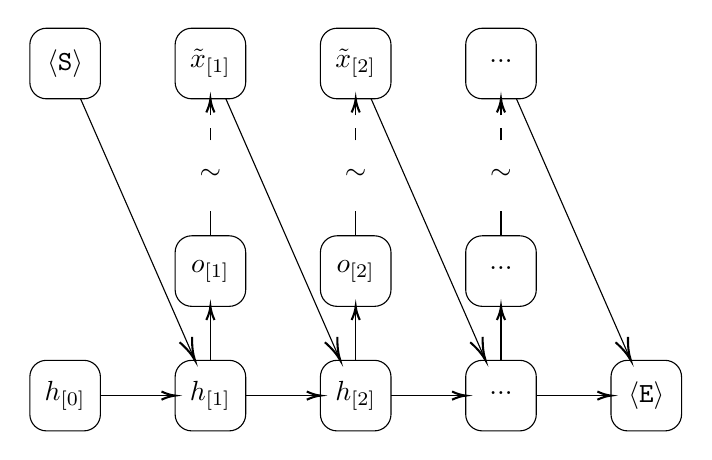
\begin{tikzpicture}[x=0.75pt,y=0.75pt,yscale=-1,xscale=1]
%uncomment if require: \path (0,235); %set diagram left start at 0, and has height of 235


% Text Node
\draw  [fill={rgb, 255:red, 255; green, 255; blue, 255 }  ,fill opacity=1 ]  (88,201) .. controls (88,196.58) and (91.58,193) .. (96,193) -- (114,193) .. controls (118.42,193) and (122,196.58) .. (122,201) -- (122,219) .. controls (122,223.42) and (118.42,227) .. (114,227) -- (96,227) .. controls (91.58,227) and (88,223.42) .. (88,219) -- cycle  ;
\draw (105,210) node   [align=left] {\begin{minipage}[lt]{20.400000000000002pt}\setlength\topsep{0pt}
\begin{center}
$\displaystyle \boldsymbol{h}_{[ 1]}$
\end{center}

\end{minipage}};
% Text Node
\draw    (18,201) .. controls (18,196.58) and (21.58,193) .. (26,193) -- (44,193) .. controls (48.42,193) and (52,196.58) .. (52,201) -- (52,219) .. controls (52,223.42) and (48.42,227) .. (44,227) -- (26,227) .. controls (21.58,227) and (18,223.42) .. (18,219) -- cycle  ;
\draw (35,210) node   [align=left] {\begin{minipage}[lt]{20.400000000000002pt}\setlength\topsep{0pt}
\begin{center}
$\displaystyle \boldsymbol{h}_{[ 0]}$
\end{center}

\end{minipage}};
% Text Node
\draw    (88,141) .. controls (88,136.58) and (91.58,133) .. (96,133) -- (114,133) .. controls (118.42,133) and (122,136.58) .. (122,141) -- (122,159) .. controls (122,163.42) and (118.42,167) .. (114,167) -- (96,167) .. controls (91.58,167) and (88,163.42) .. (88,159) -- cycle  ;
\draw (105,150) node   [align=left] {\begin{minipage}[lt]{20.400000000000002pt}\setlength\topsep{0pt}
\begin{center}
$\displaystyle \boldsymbol{o}_{[ 1]}$
\end{center}

\end{minipage}};
% Text Node
\draw (105,104) node   [align=left] {\begin{minipage}[lt]{20.400000000000002pt}\setlength\topsep{0pt}
\begin{center}
$\displaystyle \sim $
\end{center}

\end{minipage}};
% Text Node
\draw    (88,41) .. controls (88,36.58) and (91.58,33) .. (96,33) -- (114,33) .. controls (118.42,33) and (122,36.58) .. (122,41) -- (122,59) .. controls (122,63.42) and (118.42,67) .. (114,67) -- (96,67) .. controls (91.58,67) and (88,63.42) .. (88,59) -- cycle  ;
\draw (105,50) node   [align=left] {\begin{minipage}[lt]{20.400000000000002pt}\setlength\topsep{0pt}
\begin{center}
$\displaystyle \boldsymbol{\tilde{x}}$$\displaystyle _{[ 1]}$
\end{center}

\end{minipage}};
% Text Node
\draw  [fill={rgb, 255:red, 255; green, 255; blue, 255 }  ,fill opacity=1 ]  (158,201) .. controls (158,196.58) and (161.58,193) .. (166,193) -- (184,193) .. controls (188.42,193) and (192,196.58) .. (192,201) -- (192,219) .. controls (192,223.42) and (188.42,227) .. (184,227) -- (166,227) .. controls (161.58,227) and (158,223.42) .. (158,219) -- cycle  ;
\draw (175,210) node   [align=left] {\begin{minipage}[lt]{20.400000000000002pt}\setlength\topsep{0pt}
\begin{center}
$\displaystyle \boldsymbol{h}_{[ 2]}$
\end{center}

\end{minipage}};
% Text Node
\draw    (158,141) .. controls (158,136.58) and (161.58,133) .. (166,133) -- (184,133) .. controls (188.42,133) and (192,136.58) .. (192,141) -- (192,159) .. controls (192,163.42) and (188.42,167) .. (184,167) -- (166,167) .. controls (161.58,167) and (158,163.42) .. (158,159) -- cycle  ;
\draw (175,150) node   [align=left] {\begin{minipage}[lt]{20.400000000000002pt}\setlength\topsep{0pt}
\begin{center}
$\displaystyle \boldsymbol{o}_{[ 2]}$
\end{center}

\end{minipage}};
% Text Node
\draw (175,104) node   [align=left] {\begin{minipage}[lt]{20.400000000000002pt}\setlength\topsep{0pt}
\begin{center}
$\displaystyle \sim $
\end{center}

\end{minipage}};
% Text Node
\draw    (158,41) .. controls (158,36.58) and (161.58,33) .. (166,33) -- (184,33) .. controls (188.42,33) and (192,36.58) .. (192,41) -- (192,59) .. controls (192,63.42) and (188.42,67) .. (184,67) -- (166,67) .. controls (161.58,67) and (158,63.42) .. (158,59) -- cycle  ;
\draw (175,50) node   [align=left] {\begin{minipage}[lt]{20.400000000000002pt}\setlength\topsep{0pt}
\begin{center}
$\displaystyle \boldsymbol{\tilde{x}}_{[ 2]}$
\end{center}

\end{minipage}};
% Text Node
\draw  [fill={rgb, 255:red, 255; green, 255; blue, 255 }  ,fill opacity=1 ]  (228,201) .. controls (228,196.58) and (231.58,193) .. (236,193) -- (254,193) .. controls (258.42,193) and (262,196.58) .. (262,201) -- (262,219) .. controls (262,223.42) and (258.42,227) .. (254,227) -- (236,227) .. controls (231.58,227) and (228,223.42) .. (228,219) -- cycle  ;
\draw (245,210) node   [align=left] {\begin{minipage}[lt]{20.400000000000002pt}\setlength\topsep{0pt}
\begin{center}
$\displaystyle ...$
\end{center}

\end{minipage}};
% Text Node
\draw    (228,141) .. controls (228,136.58) and (231.58,133) .. (236,133) -- (254,133) .. controls (258.42,133) and (262,136.58) .. (262,141) -- (262,159) .. controls (262,163.42) and (258.42,167) .. (254,167) -- (236,167) .. controls (231.58,167) and (228,163.42) .. (228,159) -- cycle  ;
\draw (245,150) node   [align=left] {\begin{minipage}[lt]{20.400000000000002pt}\setlength\topsep{0pt}
\begin{center}
$\displaystyle ...$
\end{center}

\end{minipage}};
% Text Node
\draw (245,104) node   [align=left] {\begin{minipage}[lt]{20.400000000000002pt}\setlength\topsep{0pt}
\begin{center}
$\displaystyle \sim $
\end{center}

\end{minipage}};
% Text Node
\draw    (228,41) .. controls (228,36.58) and (231.58,33) .. (236,33) -- (254,33) .. controls (258.42,33) and (262,36.58) .. (262,41) -- (262,59) .. controls (262,63.42) and (258.42,67) .. (254,67) -- (236,67) .. controls (231.58,67) and (228,63.42) .. (228,59) -- cycle  ;
\draw (245,50) node   [align=left] {\begin{minipage}[lt]{20.400000000000002pt}\setlength\topsep{0pt}
\begin{center}
$\displaystyle ...$
\end{center}

\end{minipage}};
% Text Node
\draw  [fill={rgb, 255:red, 255; green, 255; blue, 255 }  ,fill opacity=1 ]  (298,201) .. controls (298,196.58) and (301.58,193) .. (306,193) -- (324,193) .. controls (328.42,193) and (332,196.58) .. (332,201) -- (332,219) .. controls (332,223.42) and (328.42,227) .. (324,227) -- (306,227) .. controls (301.58,227) and (298,223.42) .. (298,219) -- cycle  ;
\draw (315,210) node   [align=left] {\begin{minipage}[lt]{20.400000000000002pt}\setlength\topsep{0pt}
\begin{center}
$\displaystyle \langle \mathtt{E} \rangle $
\end{center}

\end{minipage}};
% Text Node
\draw    (18,41) .. controls (18,36.58) and (21.58,33) .. (26,33) -- (44,33) .. controls (48.42,33) and (52,36.58) .. (52,41) -- (52,59) .. controls (52,63.42) and (48.42,67) .. (44,67) -- (26,67) .. controls (21.58,67) and (18,63.42) .. (18,59) -- cycle  ;
\draw (35,50) node   [align=left] {\begin{minipage}[lt]{20.400000000000002pt}\setlength\topsep{0pt}
\begin{center}
$\displaystyle \langle \mathtt{S} \rangle $
\end{center}

\end{minipage}};
% Connection
\draw    (52,210) -- (86,210) ;
\draw [shift={(88,210)}, rotate = 180] [color={rgb, 255:red, 0; green, 0; blue, 0 }  ][line width=0.75]    (6.56,-1.97) .. controls (4.17,-0.84) and (1.99,-0.18) .. (0,0) .. controls (1.99,0.18) and (4.17,0.84) .. (6.56,1.97)   ;
% Connection
\draw    (105,193) -- (105,169) ;
\draw [shift={(105,167)}, rotate = 450] [color={rgb, 255:red, 0; green, 0; blue, 0 }  ][line width=0.75]    (6.56,-1.97) .. controls (4.17,-0.84) and (1.99,-0.18) .. (0,0) .. controls (1.99,0.18) and (4.17,0.84) .. (6.56,1.97)   ;
% Connection
\draw    (105,133) -- (105,121) ;
% Connection
\draw    (175,193) -- (175,169) ;
\draw [shift={(175,167)}, rotate = 450] [color={rgb, 255:red, 0; green, 0; blue, 0 }  ][line width=0.75]    (6.56,-1.97) .. controls (4.17,-0.84) and (1.99,-0.18) .. (0,0) .. controls (1.99,0.18) and (4.17,0.84) .. (6.56,1.97)   ;
% Connection
\draw    (175,133) -- (175,121) ;
% Connection
\draw    (122,210) -- (156,210) ;
\draw [shift={(158,210)}, rotate = 180] [color={rgb, 255:red, 0; green, 0; blue, 0 }  ][line width=0.75]    (6.56,-1.97) .. controls (4.17,-0.84) and (1.99,-0.18) .. (0,0) .. controls (1.99,0.18) and (4.17,0.84) .. (6.56,1.97)   ;
% Connection
\draw    (245,193) -- (245,169) ;
\draw [shift={(245,167)}, rotate = 450] [color={rgb, 255:red, 0; green, 0; blue, 0 }  ][line width=0.75]    (6.56,-1.97) .. controls (4.17,-0.84) and (1.99,-0.18) .. (0,0) .. controls (1.99,0.18) and (4.17,0.84) .. (6.56,1.97)   ;
% Connection
\draw    (245,133) -- (245,121) ;
% Connection
\draw    (192,210) -- (226,210) ;
\draw [shift={(228,210)}, rotate = 180] [color={rgb, 255:red, 0; green, 0; blue, 0 }  ][line width=0.75]    (6.56,-1.97) .. controls (4.17,-0.84) and (1.99,-0.18) .. (0,0) .. controls (1.99,0.18) and (4.17,0.84) .. (6.56,1.97)   ;
% Connection
\draw    (262,210) -- (296,210) ;
\draw [shift={(298,210)}, rotate = 180] [color={rgb, 255:red, 0; green, 0; blue, 0 }  ][line width=0.75]    (6.56,-1.97) .. controls (4.17,-0.84) and (1.99,-0.18) .. (0,0) .. controls (1.99,0.18) and (4.17,0.84) .. (6.56,1.97)   ;
% Connection
\draw  [dash pattern={on 4.5pt off 4.5pt}]  (105,87) -- (105,69) ;
\draw [shift={(105,67)}, rotate = 450] [color={rgb, 255:red, 0; green, 0; blue, 0 }  ][line width=0.75]    (6.56,-1.97) .. controls (4.17,-0.84) and (1.99,-0.18) .. (0,0) .. controls (1.99,0.18) and (4.17,0.84) .. (6.56,1.97)   ;
% Connection
\draw  [dash pattern={on 4.5pt off 4.5pt}]  (175,87) -- (175,69) ;
\draw [shift={(175,67)}, rotate = 450] [color={rgb, 255:red, 0; green, 0; blue, 0 }  ][line width=0.75]    (6.56,-1.97) .. controls (4.17,-0.84) and (1.99,-0.18) .. (0,0) .. controls (1.99,0.18) and (4.17,0.84) .. (6.56,1.97)   ;
% Connection
\draw  [dash pattern={on 4.5pt off 4.5pt}]  (245,87) -- (245,69) ;
\draw [shift={(245,67)}, rotate = 450] [color={rgb, 255:red, 0; green, 0; blue, 0 }  ][line width=0.75]    (6.56,-1.97) .. controls (4.17,-0.84) and (1.99,-0.18) .. (0,0) .. controls (1.99,0.18) and (4.17,0.84) .. (6.56,1.97)   ;
% Connection
\draw    (112.44,67) -- (166.76,191.17) ;
\draw [shift={(167.56,193)}, rotate = 246.37] [color={rgb, 255:red, 0; green, 0; blue, 0 }  ][line width=0.75]    (10.93,-3.29) .. controls (6.95,-1.4) and (3.31,-0.3) .. (0,0) .. controls (3.31,0.3) and (6.95,1.4) .. (10.93,3.29)   ;
% Connection
\draw    (182.44,67) -- (236.76,191.17) ;
\draw [shift={(237.56,193)}, rotate = 246.37] [color={rgb, 255:red, 0; green, 0; blue, 0 }  ][line width=0.75]    (10.93,-3.29) .. controls (6.95,-1.4) and (3.31,-0.3) .. (0,0) .. controls (3.31,0.3) and (6.95,1.4) .. (10.93,3.29)   ;
% Connection
\draw    (42.44,67) -- (96.76,191.17) ;
\draw [shift={(97.56,193)}, rotate = 246.37] [color={rgb, 255:red, 0; green, 0; blue, 0 }  ][line width=0.75]    (10.93,-3.29) .. controls (6.95,-1.4) and (3.31,-0.3) .. (0,0) .. controls (3.31,0.3) and (6.95,1.4) .. (10.93,3.29)   ;
% Connection
\draw    (252.44,67) -- (306.76,191.17) ;
\draw [shift={(307.56,193)}, rotate = 246.37] [color={rgb, 255:red, 0; green, 0; blue, 0 }  ][line width=0.75]    (10.93,-3.29) .. controls (6.95,-1.4) and (3.31,-0.3) .. (0,0) .. controls (3.31,0.3) and (6.95,1.4) .. (10.93,3.29)   ;

\end{tikzpicture}}
    \caption{An example of training a recurrent neural network for learning an autoregressive distribution. The dashed arrows indicate non-differentiable operations.}
    \label{fig:rnn-autoregressive}
\end{figure*}
During training, the sampling process breaks the differentiability of the model. Hence, one resorts to reparameterization \citep{jang2017gumbel} or differentiates the output $\Elem{o}{t}$ instead of the hard sample \citep{bengio2013straighttrough}. Another option during training is \emph{teacher forcing} \citep{williams1989teacherforcing}: in this case, the knowledge of the elements of the sequence during training is exploited, by feeding the ground truth sequence element (instead of the sampled value) as the input for the next sequence. Both strategies have advantages and disadvantages: teacher forcing learns faster initially, but does not expose the network to its own errors, thus it can be less precise at generation time. Often, a combination of the two is used.
\begin{figure*}[h!]
    \centering
    \resizebox{.7\textwidth}{!}{

\tikzset{every picture/.style={line width=0.75pt}} %set default line width to 0.75pt

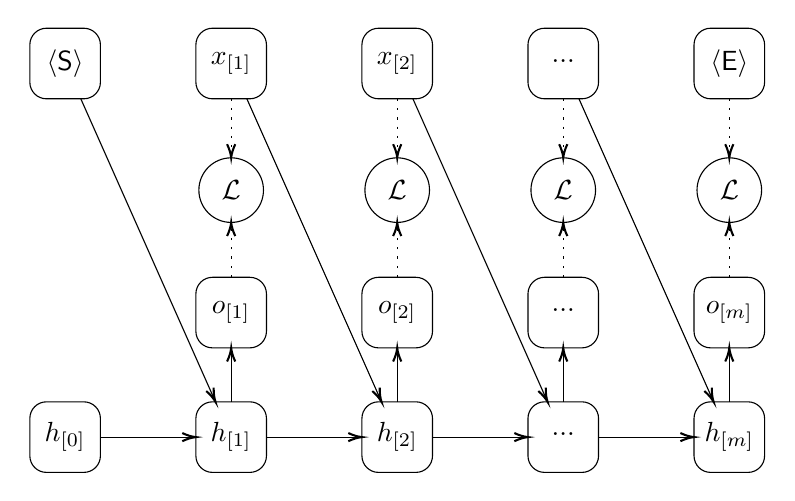
\begin{tikzpicture}[x=0.75pt,y=0.75pt,yscale=-1,xscale=1]
%uncomment if require: \path (0,259); %set diagram left start at 0, and has height of 259


% Text Node
\draw  [fill={rgb, 255:red, 255; green, 255; blue, 255 }  ,fill opacity=1 ]  (138,221) .. controls (138,216.58) and (141.58,213) .. (146,213) -- (164,213) .. controls (168.42,213) and (172,216.58) .. (172,221) -- (172,239) .. controls (172,243.42) and (168.42,247) .. (164,247) -- (146,247) .. controls (141.58,247) and (138,243.42) .. (138,239) -- cycle  ;
\draw (155,230) node   [align=left] {\begin{minipage}[lt]{20.400000000000002pt}\setlength\topsep{0pt}
\begin{center}
$\displaystyle \boldsymbol{h}_{[ 1]}$
\end{center}

\end{minipage}};
% Text Node
\draw    (58,221) .. controls (58,216.58) and (61.58,213) .. (66,213) -- (84,213) .. controls (88.42,213) and (92,216.58) .. (92,221) -- (92,239) .. controls (92,243.42) and (88.42,247) .. (84,247) -- (66,247) .. controls (61.58,247) and (58,243.42) .. (58,239) -- cycle  ;
\draw (75,230) node   [align=left] {\begin{minipage}[lt]{20.400000000000002pt}\setlength\topsep{0pt}
\begin{center}
$\displaystyle \boldsymbol{h}_{[ 0]}$
\end{center}

\end{minipage}};
% Text Node
\draw    (138,161) .. controls (138,156.58) and (141.58,153) .. (146,153) -- (164,153) .. controls (168.42,153) and (172,156.58) .. (172,161) -- (172,179) .. controls (172,183.42) and (168.42,187) .. (164,187) -- (146,187) .. controls (141.58,187) and (138,183.42) .. (138,179) -- cycle  ;
\draw (155,170) node   [align=left] {\begin{minipage}[lt]{20.400000000000002pt}\setlength\topsep{0pt}
\begin{center}
$\displaystyle \boldsymbol{o}_{[ 1]}$
\end{center}

\end{minipage}};
% Text Node
\draw    (138,41) .. controls (138,36.58) and (141.58,33) .. (146,33) -- (164,33) .. controls (168.42,33) and (172,36.58) .. (172,41) -- (172,59) .. controls (172,63.42) and (168.42,67) .. (164,67) -- (146,67) .. controls (141.58,67) and (138,63.42) .. (138,59) -- cycle  ;
\draw (155,50) node   [align=left] {\begin{minipage}[lt]{20.400000000000002pt}\setlength\topsep{0pt}
\begin{center}
$\displaystyle \boldsymbol{x}_{[ 1]}$
\end{center}

\end{minipage}};
% Text Node
\draw  [fill={rgb, 255:red, 255; green, 255; blue, 255 }  ,fill opacity=1 ]  (218,221) .. controls (218,216.58) and (221.58,213) .. (226,213) -- (244,213) .. controls (248.42,213) and (252,216.58) .. (252,221) -- (252,239) .. controls (252,243.42) and (248.42,247) .. (244,247) -- (226,247) .. controls (221.58,247) and (218,243.42) .. (218,239) -- cycle  ;
\draw (235,230) node   [align=left] {\begin{minipage}[lt]{20.400000000000002pt}\setlength\topsep{0pt}
\begin{center}
$\displaystyle \boldsymbol{h}_{[ 2]}$
\end{center}

\end{minipage}};
% Text Node
\draw    (218,161) .. controls (218,156.58) and (221.58,153) .. (226,153) -- (244,153) .. controls (248.42,153) and (252,156.58) .. (252,161) -- (252,179) .. controls (252,183.42) and (248.42,187) .. (244,187) -- (226,187) .. controls (221.58,187) and (218,183.42) .. (218,179) -- cycle  ;
\draw (235,170) node   [align=left] {\begin{minipage}[lt]{20.400000000000002pt}\setlength\topsep{0pt}
\begin{center}
$\displaystyle \boldsymbol{o}_{[ 2]}$
\end{center}

\end{minipage}};
% Text Node
\draw    (218,41) .. controls (218,36.58) and (221.58,33) .. (226,33) -- (244,33) .. controls (248.42,33) and (252,36.58) .. (252,41) -- (252,59) .. controls (252,63.42) and (248.42,67) .. (244,67) -- (226,67) .. controls (221.58,67) and (218,63.42) .. (218,59) -- cycle  ;
\draw (235,50) node   [align=left] {\begin{minipage}[lt]{20.400000000000002pt}\setlength\topsep{0pt}
\begin{center}
$\displaystyle \boldsymbol{x}_{[ 2]}$
\end{center}

\end{minipage}};
% Text Node
\draw  [fill={rgb, 255:red, 255; green, 255; blue, 255 }  ,fill opacity=1 ]  (298,221) .. controls (298,216.58) and (301.58,213) .. (306,213) -- (324,213) .. controls (328.42,213) and (332,216.58) .. (332,221) -- (332,239) .. controls (332,243.42) and (328.42,247) .. (324,247) -- (306,247) .. controls (301.58,247) and (298,243.42) .. (298,239) -- cycle  ;
\draw (315,230) node   [align=left] {\begin{minipage}[lt]{20.400000000000002pt}\setlength\topsep{0pt}
\begin{center}
$\displaystyle ...$
\end{center}

\end{minipage}};
% Text Node
\draw    (298,161) .. controls (298,156.58) and (301.58,153) .. (306,153) -- (324,153) .. controls (328.42,153) and (332,156.58) .. (332,161) -- (332,179) .. controls (332,183.42) and (328.42,187) .. (324,187) -- (306,187) .. controls (301.58,187) and (298,183.42) .. (298,179) -- cycle  ;
\draw (315,170) node   [align=left] {\begin{minipage}[lt]{20.400000000000002pt}\setlength\topsep{0pt}
\begin{center}
$\displaystyle ...$
\end{center}

\end{minipage}};
% Text Node
\draw    (298,41) .. controls (298,36.58) and (301.58,33) .. (306,33) -- (324,33) .. controls (328.42,33) and (332,36.58) .. (332,41) -- (332,59) .. controls (332,63.42) and (328.42,67) .. (324,67) -- (306,67) .. controls (301.58,67) and (298,63.42) .. (298,59) -- cycle  ;
\draw (315,50) node   [align=left] {\begin{minipage}[lt]{20.400000000000002pt}\setlength\topsep{0pt}
\begin{center}
$\displaystyle ...$
\end{center}

\end{minipage}};
% Text Node
\draw  [fill={rgb, 255:red, 255; green, 255; blue, 255 }  ,fill opacity=1 ]  (378,221) .. controls (378,216.58) and (381.58,213) .. (386,213) -- (404,213) .. controls (408.42,213) and (412,216.58) .. (412,221) -- (412,239) .. controls (412,243.42) and (408.42,247) .. (404,247) -- (386,247) .. controls (381.58,247) and (378,243.42) .. (378,239) -- cycle  ;
\draw (395,230) node   [align=left] {\begin{minipage}[lt]{20.400000000000002pt}\setlength\topsep{0pt}
\begin{center}
$\displaystyle \boldsymbol{h}_{[ m]}$
\end{center}

\end{minipage}};
% Text Node
\draw    (378,161) .. controls (378,156.58) and (381.58,153) .. (386,153) -- (404,153) .. controls (408.42,153) and (412,156.58) .. (412,161) -- (412,179) .. controls (412,183.42) and (408.42,187) .. (404,187) -- (386,187) .. controls (381.58,187) and (378,183.42) .. (378,179) -- cycle  ;
\draw (395,170) node   [align=left] {\begin{minipage}[lt]{20.400000000000002pt}\setlength\topsep{0pt}
\begin{center}
$\displaystyle \boldsymbol{o}_{[ m]}$
\end{center}

\end{minipage}};
% Text Node
\draw    (378,41) .. controls (378,36.58) and (381.58,33) .. (386,33) -- (404,33) .. controls (408.42,33) and (412,36.58) .. (412,41) -- (412,59) .. controls (412,63.42) and (408.42,67) .. (404,67) -- (386,67) .. controls (381.58,67) and (378,63.42) .. (378,59) -- cycle  ;
\draw (395,50) node   [align=left] {\begin{minipage}[lt]{20.400000000000002pt}\setlength\topsep{0pt}
\begin{center}
$\displaystyle \langle \mathsf{E} \rangle $
\end{center}

\end{minipage}};
% Text Node
\draw    (58,41) .. controls (58,36.58) and (61.58,33) .. (66,33) -- (84,33) .. controls (88.42,33) and (92,36.58) .. (92,41) -- (92,59) .. controls (92,63.42) and (88.42,67) .. (84,67) -- (66,67) .. controls (61.58,67) and (58,63.42) .. (58,59) -- cycle  ;
\draw (75,50) node   [align=left] {\begin{minipage}[lt]{20.400000000000002pt}\setlength\topsep{0pt}
\begin{center}
$\displaystyle \langle \mathsf{S} \rangle $
\end{center}

\end{minipage}};
% Text Node
\draw    (395, 111) circle [x radius= 15.56, y radius= 15.56]   ;
\draw (395,111) node   [align=left] {\begin{minipage}[lt]{13.735995849609345pt}\setlength\topsep{0pt}
\begin{center}
$\displaystyle \mathcal{L}$
\end{center}

\end{minipage}};
% Text Node
\draw    (315, 111) circle [x radius= 15.56, y radius= 15.56]   ;
\draw (315,111) node   [align=left] {\begin{minipage}[lt]{13.735995849609345pt}\setlength\topsep{0pt}
\begin{center}
$\displaystyle \mathcal{L}$
\end{center}

\end{minipage}};
% Text Node
\draw    (235, 111) circle [x radius= 15.56, y radius= 15.56]   ;
\draw (235,111) node   [align=left] {\begin{minipage}[lt]{13.735995849609345pt}\setlength\topsep{0pt}
\begin{center}
$\displaystyle \mathcal{L}$
\end{center}

\end{minipage}};
% Text Node
\draw    (155, 111) circle [x radius= 15.56, y radius= 15.56]   ;
\draw (155,111) node   [align=left] {\begin{minipage}[lt]{13.735995849609345pt}\setlength\topsep{0pt}
\begin{center}
$\displaystyle \mathcal{L}$
\end{center}

\end{minipage}};
% Connection
\draw    (92,230) -- (136,230) ;
\draw [shift={(138,230)}, rotate = 180] [color={rgb, 255:red, 0; green, 0; blue, 0 }  ][line width=0.75]    (6.56,-1.97) .. controls (4.17,-0.84) and (1.99,-0.18) .. (0,0) .. controls (1.99,0.18) and (4.17,0.84) .. (6.56,1.97)   ;
% Connection
\draw    (155,213) -- (155,189) ;
\draw [shift={(155,187)}, rotate = 450] [color={rgb, 255:red, 0; green, 0; blue, 0 }  ][line width=0.75]    (6.56,-1.97) .. controls (4.17,-0.84) and (1.99,-0.18) .. (0,0) .. controls (1.99,0.18) and (4.17,0.84) .. (6.56,1.97)   ;
% Connection
\draw    (235,213) -- (235,189) ;
\draw [shift={(235,187)}, rotate = 450] [color={rgb, 255:red, 0; green, 0; blue, 0 }  ][line width=0.75]    (6.56,-1.97) .. controls (4.17,-0.84) and (1.99,-0.18) .. (0,0) .. controls (1.99,0.18) and (4.17,0.84) .. (6.56,1.97)   ;
% Connection
\draw    (172,230) -- (216,230) ;
\draw [shift={(218,230)}, rotate = 180] [color={rgb, 255:red, 0; green, 0; blue, 0 }  ][line width=0.75]    (6.56,-1.97) .. controls (4.17,-0.84) and (1.99,-0.18) .. (0,0) .. controls (1.99,0.18) and (4.17,0.84) .. (6.56,1.97)   ;
% Connection
\draw    (315,213) -- (315,189) ;
\draw [shift={(315,187)}, rotate = 450] [color={rgb, 255:red, 0; green, 0; blue, 0 }  ][line width=0.75]    (6.56,-1.97) .. controls (4.17,-0.84) and (1.99,-0.18) .. (0,0) .. controls (1.99,0.18) and (4.17,0.84) .. (6.56,1.97)   ;
% Connection
\draw    (252,230) -- (296,230) ;
\draw [shift={(298,230)}, rotate = 180] [color={rgb, 255:red, 0; green, 0; blue, 0 }  ][line width=0.75]    (6.56,-1.97) .. controls (4.17,-0.84) and (1.99,-0.18) .. (0,0) .. controls (1.99,0.18) and (4.17,0.84) .. (6.56,1.97)   ;
% Connection
\draw    (395,213) -- (395,189) ;
\draw [shift={(395,187)}, rotate = 450] [color={rgb, 255:red, 0; green, 0; blue, 0 }  ][line width=0.75]    (6.56,-1.97) .. controls (4.17,-0.84) and (1.99,-0.18) .. (0,0) .. controls (1.99,0.18) and (4.17,0.84) .. (6.56,1.97)   ;
% Connection
\draw    (332,230) -- (376,230) ;
\draw [shift={(378,230)}, rotate = 180] [color={rgb, 255:red, 0; green, 0; blue, 0 }  ][line width=0.75]    (6.56,-1.97) .. controls (4.17,-0.84) and (1.99,-0.18) .. (0,0) .. controls (1.99,0.18) and (4.17,0.84) .. (6.56,1.97)   ;
% Connection
\draw    (82.56,67) -- (146.63,211.17) ;
\draw [shift={(147.44,213)}, rotate = 246.04000000000002] [color={rgb, 255:red, 0; green, 0; blue, 0 }  ][line width=0.75]    (6.56,-1.97) .. controls (4.17,-0.84) and (1.99,-0.18) .. (0,0) .. controls (1.99,0.18) and (4.17,0.84) .. (6.56,1.97)   ;
% Connection
\draw    (162.56,67) -- (226.63,211.17) ;
\draw [shift={(227.44,213)}, rotate = 246.04000000000002] [color={rgb, 255:red, 0; green, 0; blue, 0 }  ][line width=0.75]    (6.56,-1.97) .. controls (4.17,-0.84) and (1.99,-0.18) .. (0,0) .. controls (1.99,0.18) and (4.17,0.84) .. (6.56,1.97)   ;
% Connection
\draw    (242.56,67) -- (306.63,211.17) ;
\draw [shift={(307.44,213)}, rotate = 246.04000000000002] [color={rgb, 255:red, 0; green, 0; blue, 0 }  ][line width=0.75]    (6.56,-1.97) .. controls (4.17,-0.84) and (1.99,-0.18) .. (0,0) .. controls (1.99,0.18) and (4.17,0.84) .. (6.56,1.97)   ;
% Connection
\draw    (322.56,67) -- (386.63,211.17) ;
\draw [shift={(387.44,213)}, rotate = 246.04000000000002] [color={rgb, 255:red, 0; green, 0; blue, 0 }  ][line width=0.75]    (6.56,-1.97) .. controls (4.17,-0.84) and (1.99,-0.18) .. (0,0) .. controls (1.99,0.18) and (4.17,0.84) .. (6.56,1.97)   ;
% Connection
\draw  [dash pattern={on 0.84pt off 2.51pt}]  (155,153) -- (155,128.56) ;
\draw [shift={(155,126.56)}, rotate = 450] [color={rgb, 255:red, 0; green, 0; blue, 0 }  ][line width=0.75]    (6.56,-1.97) .. controls (4.17,-0.84) and (1.99,-0.18) .. (0,0) .. controls (1.99,0.18) and (4.17,0.84) .. (6.56,1.97)   ;
% Connection
\draw  [dash pattern={on 0.84pt off 2.51pt}]  (155,67) -- (155,93.44) ;
\draw [shift={(155,95.44)}, rotate = 270] [color={rgb, 255:red, 0; green, 0; blue, 0 }  ][line width=0.75]    (6.56,-1.97) .. controls (4.17,-0.84) and (1.99,-0.18) .. (0,0) .. controls (1.99,0.18) and (4.17,0.84) .. (6.56,1.97)   ;
% Connection
\draw  [dash pattern={on 0.84pt off 2.51pt}]  (235,153) -- (235,128.56) ;
\draw [shift={(235,126.56)}, rotate = 450] [color={rgb, 255:red, 0; green, 0; blue, 0 }  ][line width=0.75]    (6.56,-1.97) .. controls (4.17,-0.84) and (1.99,-0.18) .. (0,0) .. controls (1.99,0.18) and (4.17,0.84) .. (6.56,1.97)   ;
% Connection
\draw  [dash pattern={on 0.84pt off 2.51pt}]  (235,67) -- (235,93.44) ;
\draw [shift={(235,95.44)}, rotate = 270] [color={rgb, 255:red, 0; green, 0; blue, 0 }  ][line width=0.75]    (6.56,-1.97) .. controls (4.17,-0.84) and (1.99,-0.18) .. (0,0) .. controls (1.99,0.18) and (4.17,0.84) .. (6.56,1.97)   ;
% Connection
\draw  [dash pattern={on 0.84pt off 2.51pt}]  (315,153) -- (315,128.56) ;
\draw [shift={(315,126.56)}, rotate = 450] [color={rgb, 255:red, 0; green, 0; blue, 0 }  ][line width=0.75]    (6.56,-1.97) .. controls (4.17,-0.84) and (1.99,-0.18) .. (0,0) .. controls (1.99,0.18) and (4.17,0.84) .. (6.56,1.97)   ;
% Connection
\draw  [dash pattern={on 0.84pt off 2.51pt}]  (315,67) -- (315,93.44) ;
\draw [shift={(315,95.44)}, rotate = 270] [color={rgb, 255:red, 0; green, 0; blue, 0 }  ][line width=0.75]    (6.56,-1.97) .. controls (4.17,-0.84) and (1.99,-0.18) .. (0,0) .. controls (1.99,0.18) and (4.17,0.84) .. (6.56,1.97)   ;
% Connection
\draw  [dash pattern={on 0.84pt off 2.51pt}]  (395,153) -- (395,128.56) ;
\draw [shift={(395,126.56)}, rotate = 450] [color={rgb, 255:red, 0; green, 0; blue, 0 }  ][line width=0.75]    (6.56,-1.97) .. controls (4.17,-0.84) and (1.99,-0.18) .. (0,0) .. controls (1.99,0.18) and (4.17,0.84) .. (6.56,1.97)   ;
% Connection
\draw  [dash pattern={on 0.84pt off 2.51pt}]  (395,67) -- (395,93.44) ;
\draw [shift={(395,95.44)}, rotate = 270] [color={rgb, 255:red, 0; green, 0; blue, 0 }  ][line width=0.75]    (6.56,-1.97) .. controls (4.17,-0.84) and (1.99,-0.18) .. (0,0) .. controls (1.99,0.18) and (4.17,0.84) .. (6.56,1.97)   ;

\end{tikzpicture}}
    \caption{The teacher forcing strategy for training a sequence generator with RNNs.}
    \label{fig:teacher-forcing}
\end{figure*}

\section{Recursive Neural Networks} \label{sec:recnns}
A \gls{recnn} \citep{sperduti1997generalizedneuron,frasconi1998general} is a \gls{nn} architecture that can adaptively process hierarchical data. Using trees as an example, let $\Tree{T}$ be an attributed tree with $m$ nodes $\Nodes{t} = \Set{v_1, v_2, \ldots, v_m}$, and $\Vector{x}_{\Tree{t}} = \Set{\Elem{x}{v} \in \Real^d \mid v \in \Nodes{t}}$ be its set node of features. The state transition function of a \gls{recnn}, applied locally to each node $v \in \Nodes{t}$, is the following:
\begin{align*}
    \Elem{h}{v}=
    \begin{cases}
        \boldsymbol{0} & \mathrm{if}\; \Fun{ch}(v) = \emptyset\\
        \EncTrans(\Elem{x}{v}, \Elem{h}{\Tree{t}_v}) & \mathrm{otherwise},
    \end{cases}
\end{align*}
where $\Elem{h}{\Tree{t}_v} \in \Real^h$ is the hidden state of the sub-tree rooted at $v$. As with \glspl{rnn}, the state transition function $\EncTrans$ is recursive, but this time the recursion is defined over the tree structure. Specifically, to compute the hidden state of a node, the hidden state of all its children must be known in advance. The state computation starts at the leaves of the tree (where the state is initialized beforehand to make the recursion well-defined), and proceeds bottom-up until the root node is reached.
The development of \glspl{recnn} started in the middle '90s, with the introduction of the notion of generalized recursive neuron \citep{sperduti1997generalizedneuron} and the development of a general framework for learning with tree-structured data \citep{frasconi1998general}, which was later extended to more expressive classes of structures such as \glspl{dag} and \glspl{dpag}. Since then, they have been applied fruitfully in several fields, including among others Cheminformatics \citep{micheli2007introductionrecnncheminformatics,baldi2013recursiveneuralnets}, \gls{nlp} \citep{costa2000recnns,costa2003recnns,sturt2003recnns,socher2013recnnsentiment} and scene parsing \citep{socher2011parsingscenes}. Interestingly, \glspl{recnn} are also backed up by strong theoretical results, which support the generality of the structural transduction and characterize the kind of functions they can learn. Specifically, universal approximation theorems showing that \glspl{recnn} can approximate arbitrarily well any function from labeled trees to real values \citep{hammer1999recnn}, and from labeled \glspl{dpag} to real values \citep{hammer2005universal} have been proved. \glspl{recnn} can be trained with \gls{bpts} \cite{goller1996backpropstructure}, a variant of \gls{bptt} where the error of the network is propagated to the tree structure.

\subsection{Training}
Using the binary tree of Figure \ref{fig:tree} and a structure-to-element task as an example, one possible implementation of the state transition function of a \gls{recnn} is the following:
\begin{align*}
    \Elem{h}{v} &= \sigma\Par{\Matrix{W}\Elem{x}{v} + \Matrix{U}_\Fun{l}\Elem{h}{\Fun{l}(v)} + \Matrix{U}_\Fun{r}\Elem{h}{\Fun{r}(v)}},\; \forall v \in \Nodes{t}.
\end{align*}
In the above formula, $g$ can be any hidden activation function, and $\Matrix{w} \in \Real^{d \times h}$, $\Matrix{u}_\Fun{l}$, and $\Matrix{u}_\Fun{r} \in \Real^{h \times h}$, are weight matrices shared across the structure. Notice that the two weight matrices on the node children are positional, meaning that they are applied to a certain node according to its position. In the example case of a binary tree, the two functions $\Fun{l}(v)$ and $\Fun{r}(v)$ select the left and right child of a node $v$, respectively, if they exist. Figure \ref{fig:recnn} shows the unfolded \gls{recnn} over the tree. The final output of the entire structure is obtained using the hidden state of the root node $v_1$ as:
$$\Vector{o} = g\Par{\Elem{h}{v_1}},$$
where $\Vector{o} \in \Real^y$ is the output of the network and $g$ can be any downstream network such as a simple output layer, or a more complex neural network. For structure-to-structure tasks, the output is calculated node-wise as follows:
$$\Elem{o}{v} = g\Par{\Elem{h}{v}},\; \forall v \in \Nodes{t}.$$
Notably, the order by which the hidden states need to be calculated (the numbers at the left of the hidden states in the figure) must be respected to ensure that the recursive process is well-defined. The state of nodes with the same ordering can be calculated in parallel according to the tree structure, which makes \glspl{recnn} more efficient than \glspl{rnn} when compared on structures with the same number of elements.
\begin{figure*}[h!]
    \centering
    \resizebox{.5\textwidth}{!}{

\tikzset{every picture/.style={line width=0.75pt}} %set default line width to 0.75pt

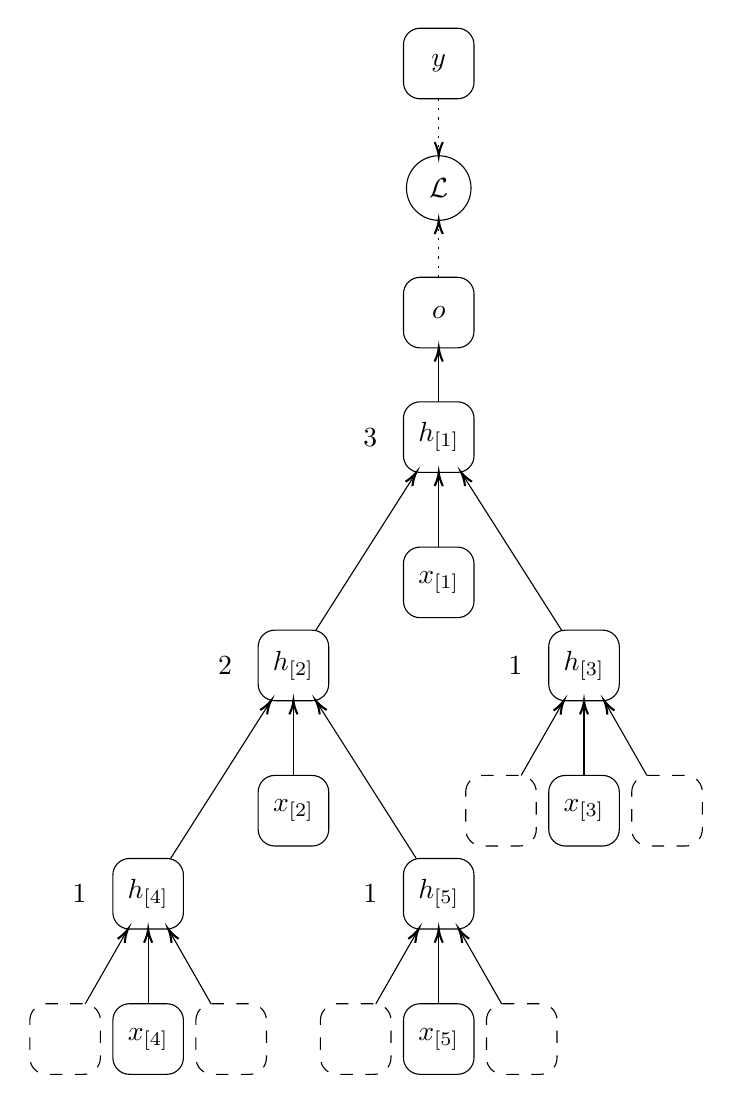
\begin{tikzpicture}[x=0.75pt,y=0.75pt,yscale=-1,xscale=1]
%uncomment if require: \path (0,532); %set diagram left start at 0, and has height of 532


% Text Node
\draw  [fill={rgb, 255:red, 255; green, 255; blue, 255 }  ,fill opacity=1 ]  (198,421) .. controls (198,416.58) and (201.58,413) .. (206,413) -- (224,413) .. controls (228.42,413) and (232,416.58) .. (232,421) -- (232,439) .. controls (232,443.42) and (228.42,447) .. (224,447) -- (206,447) .. controls (201.58,447) and (198,443.42) .. (198,439) -- cycle  ;
\draw (215,430) node   [align=left] {\begin{minipage}[lt]{20.400000000000002pt}\setlength\topsep{0pt}
\begin{center}
$\displaystyle \boldsymbol{h}_{[ 4]}$
\end{center}

\end{minipage}};
% Text Node
\draw  [fill={rgb, 255:red, 255; green, 255; blue, 255 }  ,fill opacity=1 ]  (338,421) .. controls (338,416.58) and (341.58,413) .. (346,413) -- (364,413) .. controls (368.42,413) and (372,416.58) .. (372,421) -- (372,439) .. controls (372,443.42) and (368.42,447) .. (364,447) -- (346,447) .. controls (341.58,447) and (338,443.42) .. (338,439) -- cycle  ;
\draw (355,430) node   [align=left] {\begin{minipage}[lt]{20.400000000000002pt}\setlength\topsep{0pt}
\begin{center}
$\displaystyle \boldsymbol{h}_{[ 5]}$
\end{center}

\end{minipage}};
% Text Node
\draw  [fill={rgb, 255:red, 255; green, 255; blue, 255 }  ,fill opacity=1 ]  (268,311) .. controls (268,306.58) and (271.58,303) .. (276,303) -- (294,303) .. controls (298.42,303) and (302,306.58) .. (302,311) -- (302,329) .. controls (302,333.42) and (298.42,337) .. (294,337) -- (276,337) .. controls (271.58,337) and (268,333.42) .. (268,329) -- cycle  ;
\draw (285,320) node   [align=left] {\begin{minipage}[lt]{20.400000000000002pt}\setlength\topsep{0pt}
\begin{center}
$\displaystyle \boldsymbol{h}_{[ 2]}$
\end{center}

\end{minipage}};
% Text Node
\draw  [fill={rgb, 255:red, 255; green, 255; blue, 255 }  ,fill opacity=1 ]  (338,201) .. controls (338,196.58) and (341.58,193) .. (346,193) -- (364,193) .. controls (368.42,193) and (372,196.58) .. (372,201) -- (372,219) .. controls (372,223.42) and (368.42,227) .. (364,227) -- (346,227) .. controls (341.58,227) and (338,223.42) .. (338,219) -- cycle  ;
\draw (355,210) node   [align=left] {\begin{minipage}[lt]{20.400000000000002pt}\setlength\topsep{0pt}
\begin{center}
$\displaystyle \boldsymbol{h}_{[ 1]}$
\end{center}

\end{minipage}};
% Text Node
\draw  [fill={rgb, 255:red, 255; green, 255; blue, 255 }  ,fill opacity=1 ]  (408,311) .. controls (408,306.58) and (411.58,303) .. (416,303) -- (434,303) .. controls (438.42,303) and (442,306.58) .. (442,311) -- (442,329) .. controls (442,333.42) and (438.42,337) .. (434,337) -- (416,337) .. controls (411.58,337) and (408,333.42) .. (408,329) -- cycle  ;
\draw (425,320) node   [align=left] {\begin{minipage}[lt]{20.400000000000002pt}\setlength\topsep{0pt}
\begin{center}
$\displaystyle \boldsymbol{h}_{[ 3]}$
\end{center}

\end{minipage}};
% Text Node
\draw  [fill={rgb, 255:red, 255; green, 255; blue, 255 }  ,fill opacity=1 ]  (198,491) .. controls (198,486.58) and (201.58,483) .. (206,483) -- (224,483) .. controls (228.42,483) and (232,486.58) .. (232,491) -- (232,509) .. controls (232,513.42) and (228.42,517) .. (224,517) -- (206,517) .. controls (201.58,517) and (198,513.42) .. (198,509) -- cycle  ;
\draw (215,500) node   [align=left] {\begin{minipage}[lt]{20.400000000000002pt}\setlength\topsep{0pt}
\begin{center}
$\displaystyle \boldsymbol{x}_{[ 4]}$
\end{center}

\end{minipage}};
% Text Node
\draw  [fill={rgb, 255:red, 255; green, 255; blue, 255 }  ,fill opacity=1 ]  (338,491) .. controls (338,486.58) and (341.58,483) .. (346,483) -- (364,483) .. controls (368.42,483) and (372,486.58) .. (372,491) -- (372,509) .. controls (372,513.42) and (368.42,517) .. (364,517) -- (346,517) .. controls (341.58,517) and (338,513.42) .. (338,509) -- cycle  ;
\draw (355,500) node   [align=left] {\begin{minipage}[lt]{20.400000000000002pt}\setlength\topsep{0pt}
\begin{center}
$\displaystyle \boldsymbol{x}_{[ 5]}$
\end{center}

\end{minipage}};
% Text Node
\draw  [fill={rgb, 255:red, 255; green, 255; blue, 255 }  ,fill opacity=1 ]  (268,381) .. controls (268,376.58) and (271.58,373) .. (276,373) -- (294,373) .. controls (298.42,373) and (302,376.58) .. (302,381) -- (302,399) .. controls (302,403.42) and (298.42,407) .. (294,407) -- (276,407) .. controls (271.58,407) and (268,403.42) .. (268,399) -- cycle  ;
\draw (285,390) node   [align=left] {\begin{minipage}[lt]{20.400000000000002pt}\setlength\topsep{0pt}
\begin{center}
$\displaystyle \boldsymbol{x}_{[ 2]}$
\end{center}

\end{minipage}};
% Text Node
\draw  [fill={rgb, 255:red, 255; green, 255; blue, 255 }  ,fill opacity=1 ]  (338,271) .. controls (338,266.58) and (341.58,263) .. (346,263) -- (364,263) .. controls (368.42,263) and (372,266.58) .. (372,271) -- (372,289) .. controls (372,293.42) and (368.42,297) .. (364,297) -- (346,297) .. controls (341.58,297) and (338,293.42) .. (338,289) -- cycle  ;
\draw (355,280) node   [align=left] {\begin{minipage}[lt]{20.400000000000002pt}\setlength\topsep{0pt}
\begin{center}
$\displaystyle \boldsymbol{x}_{[ 1]}$
\end{center}

\end{minipage}};
% Text Node
\draw  [fill={rgb, 255:red, 255; green, 255; blue, 255 }  ,fill opacity=1 ]  (408,381) .. controls (408,376.58) and (411.58,373) .. (416,373) -- (434,373) .. controls (438.42,373) and (442,376.58) .. (442,381) -- (442,399) .. controls (442,403.42) and (438.42,407) .. (434,407) -- (416,407) .. controls (411.58,407) and (408,403.42) .. (408,399) -- cycle  ;
\draw (425,390) node   [align=left] {\begin{minipage}[lt]{20.400000000000002pt}\setlength\topsep{0pt}
\begin{center}
$\displaystyle \boldsymbol{x}_{[ 3]}$
\end{center}

\end{minipage}};
% Text Node
\draw  [fill={rgb, 255:red, 255; green, 255; blue, 255 }  ,fill opacity=1 ][dash pattern={on 4.5pt off 4.5pt}]  (238,491) .. controls (238,486.58) and (241.58,483) .. (246,483) -- (264,483) .. controls (268.42,483) and (272,486.58) .. (272,491) -- (272,509) .. controls (272,513.42) and (268.42,517) .. (264,517) -- (246,517) .. controls (241.58,517) and (238,513.42) .. (238,509) -- cycle  ;
\draw (255,500) node   [align=left] {\begin{minipage}[lt]{20.400000000000002pt}\setlength\topsep{0pt}
\begin{center}
$ $
\end{center}

\end{minipage}};
% Text Node
\draw  [fill={rgb, 255:red, 255; green, 255; blue, 255 }  ,fill opacity=1 ][dash pattern={on 4.5pt off 4.5pt}]  (158,491) .. controls (158,486.58) and (161.58,483) .. (166,483) -- (184,483) .. controls (188.42,483) and (192,486.58) .. (192,491) -- (192,509) .. controls (192,513.42) and (188.42,517) .. (184,517) -- (166,517) .. controls (161.58,517) and (158,513.42) .. (158,509) -- cycle  ;
\draw (175,500) node   [align=left] {\begin{minipage}[lt]{20.400000000000002pt}\setlength\topsep{0pt}
\begin{center}
$ $
\end{center}

\end{minipage}};
% Text Node
\draw  [fill={rgb, 255:red, 255; green, 255; blue, 255 }  ,fill opacity=1 ][dash pattern={on 4.5pt off 4.5pt}]  (298,491) .. controls (298,486.58) and (301.58,483) .. (306,483) -- (324,483) .. controls (328.42,483) and (332,486.58) .. (332,491) -- (332,509) .. controls (332,513.42) and (328.42,517) .. (324,517) -- (306,517) .. controls (301.58,517) and (298,513.42) .. (298,509) -- cycle  ;
\draw (315,500) node   [align=left] {\begin{minipage}[lt]{20.400000000000002pt}\setlength\topsep{0pt}
\begin{center}
$ $
\end{center}

\end{minipage}};
% Text Node
\draw  [fill={rgb, 255:red, 255; green, 255; blue, 255 }  ,fill opacity=1 ][dash pattern={on 4.5pt off 4.5pt}]  (378,491) .. controls (378,486.58) and (381.58,483) .. (386,483) -- (404,483) .. controls (408.42,483) and (412,486.58) .. (412,491) -- (412,509) .. controls (412,513.42) and (408.42,517) .. (404,517) -- (386,517) .. controls (381.58,517) and (378,513.42) .. (378,509) -- cycle  ;
\draw (395,500) node   [align=left] {\begin{minipage}[lt]{20.400000000000002pt}\setlength\topsep{0pt}
\begin{center}
$ $
\end{center}

\end{minipage}};
% Text Node
\draw  [fill={rgb, 255:red, 255; green, 255; blue, 255 }  ,fill opacity=1 ][dash pattern={on 4.5pt off 4.5pt}]  (368,381) .. controls (368,376.58) and (371.58,373) .. (376,373) -- (394,373) .. controls (398.42,373) and (402,376.58) .. (402,381) -- (402,399) .. controls (402,403.42) and (398.42,407) .. (394,407) -- (376,407) .. controls (371.58,407) and (368,403.42) .. (368,399) -- cycle  ;
\draw (385,390) node   [align=left] {\begin{minipage}[lt]{20.400000000000002pt}\setlength\topsep{0pt}
\begin{center}
$ $
\end{center}

\end{minipage}};
% Text Node
\draw  [fill={rgb, 255:red, 255; green, 255; blue, 255 }  ,fill opacity=1 ][dash pattern={on 4.5pt off 4.5pt}]  (448,381) .. controls (448,376.58) and (451.58,373) .. (456,373) -- (474,373) .. controls (478.42,373) and (482,376.58) .. (482,381) -- (482,399) .. controls (482,403.42) and (478.42,407) .. (474,407) -- (456,407) .. controls (451.58,407) and (448,403.42) .. (448,399) -- cycle  ;
\draw (465,390) node   [align=left] {\begin{minipage}[lt]{20.400000000000002pt}\setlength\topsep{0pt}
\begin{center}
$ $
\end{center}

\end{minipage}};
% Text Node
\draw  [fill={rgb, 255:red, 255; green, 255; blue, 255 }  ,fill opacity=1 ]  (338,141) .. controls (338,136.58) and (341.58,133) .. (346,133) -- (364,133) .. controls (368.42,133) and (372,136.58) .. (372,141) -- (372,159) .. controls (372,163.42) and (368.42,167) .. (364,167) -- (346,167) .. controls (341.58,167) and (338,163.42) .. (338,159) -- cycle  ;
\draw (355,150) node   [align=left] {\begin{minipage}[lt]{20.400000000000002pt}\setlength\topsep{0pt}
\begin{center}
$\displaystyle \boldsymbol{o}$
\end{center}

\end{minipage}};
% Text Node
\draw  [fill={rgb, 255:red, 255; green, 255; blue, 255 }  ,fill opacity=1 ]  (338,21) .. controls (338,16.58) and (341.58,13) .. (346,13) -- (364,13) .. controls (368.42,13) and (372,16.58) .. (372,21) -- (372,39) .. controls (372,43.42) and (368.42,47) .. (364,47) -- (346,47) .. controls (341.58,47) and (338,43.42) .. (338,39) -- cycle  ;
\draw (355,30) node   [align=left] {\begin{minipage}[lt]{20.400000000000002pt}\setlength\topsep{0pt}
\begin{center}
$\displaystyle \boldsymbol{y}$
\end{center}

\end{minipage}};
% Text Node
\draw    (355, 90) circle [x radius= 15.56, y radius= 15.56]   ;
\draw (355,90) node   [align=left] {\begin{minipage}[lt]{13.735995849609345pt}\setlength\topsep{0pt}
\begin{center}
$\displaystyle \mathcal{L}$
\end{center}

\end{minipage}};
% Text Node
\draw (182,430) node   [align=left] {\begin{minipage}[lt]{20.400000000000002pt}\setlength\topsep{0pt}
\begin{center}
$\displaystyle 1$
\end{center}

\end{minipage}};
% Text Node
\draw (322,430) node   [align=left] {\begin{minipage}[lt]{20.400000000000002pt}\setlength\topsep{0pt}
\begin{center}
$\displaystyle 1$
\end{center}

\end{minipage}};
% Text Node
\draw (392,320) node   [align=left] {\begin{minipage}[lt]{20.400000000000002pt}\setlength\topsep{0pt}
\begin{center}
$\displaystyle 1$
\end{center}

\end{minipage}};
% Text Node
\draw (252,320) node   [align=left] {\begin{minipage}[lt]{20.400000000000002pt}\setlength\topsep{0pt}
\begin{center}
$\displaystyle 2$
\end{center}

\end{minipage}};
% Text Node
\draw (322,210) node   [align=left] {\begin{minipage}[lt]{20.400000000000002pt}\setlength\topsep{0pt}
\begin{center}
$\displaystyle 3$
\end{center}

\end{minipage}};
% Connection
\draw    (225.82,413) -- (273.11,338.69) ;
\draw [shift={(274.18,337)}, rotate = 482.47] [color={rgb, 255:red, 0; green, 0; blue, 0 }  ][line width=0.75]    (6.56,-1.97) .. controls (4.17,-0.84) and (1.99,-0.18) .. (0,0) .. controls (1.99,0.18) and (4.17,0.84) .. (6.56,1.97)   ;
% Connection
\draw    (295.82,303) -- (343.11,228.69) ;
\draw [shift={(344.18,227)}, rotate = 482.47] [color={rgb, 255:red, 0; green, 0; blue, 0 }  ][line width=0.75]    (6.56,-1.97) .. controls (4.17,-0.84) and (1.99,-0.18) .. (0,0) .. controls (1.99,0.18) and (4.17,0.84) .. (6.56,1.97)   ;
% Connection
\draw    (344.18,413) -- (296.89,338.69) ;
\draw [shift={(295.82,337)}, rotate = 417.53] [color={rgb, 255:red, 0; green, 0; blue, 0 }  ][line width=0.75]    (6.56,-1.97) .. controls (4.17,-0.84) and (1.99,-0.18) .. (0,0) .. controls (1.99,0.18) and (4.17,0.84) .. (6.56,1.97)   ;
% Connection
\draw    (414.18,303) -- (366.89,228.69) ;
\draw [shift={(365.82,227)}, rotate = 417.53] [color={rgb, 255:red, 0; green, 0; blue, 0 }  ][line width=0.75]    (6.56,-1.97) .. controls (4.17,-0.84) and (1.99,-0.18) .. (0,0) .. controls (1.99,0.18) and (4.17,0.84) .. (6.56,1.97)   ;
% Connection
\draw    (215,483) -- (215,449) ;
\draw [shift={(215,447)}, rotate = 450] [color={rgb, 255:red, 0; green, 0; blue, 0 }  ][line width=0.75]    (6.56,-1.97) .. controls (4.17,-0.84) and (1.99,-0.18) .. (0,0) .. controls (1.99,0.18) and (4.17,0.84) .. (6.56,1.97)   ;
% Connection
\draw    (285,373) -- (285,339) ;
\draw [shift={(285,337)}, rotate = 450] [color={rgb, 255:red, 0; green, 0; blue, 0 }  ][line width=0.75]    (6.56,-1.97) .. controls (4.17,-0.84) and (1.99,-0.18) .. (0,0) .. controls (1.99,0.18) and (4.17,0.84) .. (6.56,1.97)   ;
% Connection
\draw    (355,483) -- (355,449) ;
\draw [shift={(355,447)}, rotate = 450] [color={rgb, 255:red, 0; green, 0; blue, 0 }  ][line width=0.75]    (6.56,-1.97) .. controls (4.17,-0.84) and (1.99,-0.18) .. (0,0) .. controls (1.99,0.18) and (4.17,0.84) .. (6.56,1.97)   ;
% Connection
\draw    (425,373) -- (425,339) ;
\draw [shift={(425,337)}, rotate = 450] [color={rgb, 255:red, 0; green, 0; blue, 0 }  ][line width=0.75]    (6.56,-1.97) .. controls (4.17,-0.84) and (1.99,-0.18) .. (0,0) .. controls (1.99,0.18) and (4.17,0.84) .. (6.56,1.97)   ;
% Connection
\draw    (355,263) -- (355,229) ;
\draw [shift={(355,227)}, rotate = 450] [color={rgb, 255:red, 0; green, 0; blue, 0 }  ][line width=0.75]    (6.56,-1.97) .. controls (4.17,-0.84) and (1.99,-0.18) .. (0,0) .. controls (1.99,0.18) and (4.17,0.84) .. (6.56,1.97)   ;
% Connection
\draw    (184.71,483) -- (204.29,448.74) ;
\draw [shift={(205.29,447)}, rotate = 479.74] [color={rgb, 255:red, 0; green, 0; blue, 0 }  ][line width=0.75]    (6.56,-1.97) .. controls (4.17,-0.84) and (1.99,-0.18) .. (0,0) .. controls (1.99,0.18) and (4.17,0.84) .. (6.56,1.97)   ;
% Connection
\draw    (245.29,483) -- (225.71,448.74) ;
\draw [shift={(224.71,447)}, rotate = 420.26] [color={rgb, 255:red, 0; green, 0; blue, 0 }  ][line width=0.75]    (6.56,-1.97) .. controls (4.17,-0.84) and (1.99,-0.18) .. (0,0) .. controls (1.99,0.18) and (4.17,0.84) .. (6.56,1.97)   ;
% Connection
\draw    (324.71,483) -- (344.29,448.74) ;
\draw [shift={(345.29,447)}, rotate = 479.74] [color={rgb, 255:red, 0; green, 0; blue, 0 }  ][line width=0.75]    (6.56,-1.97) .. controls (4.17,-0.84) and (1.99,-0.18) .. (0,0) .. controls (1.99,0.18) and (4.17,0.84) .. (6.56,1.97)   ;
% Connection
\draw    (385.29,483) -- (365.71,448.74) ;
\draw [shift={(364.71,447)}, rotate = 420.26] [color={rgb, 255:red, 0; green, 0; blue, 0 }  ][line width=0.75]    (6.56,-1.97) .. controls (4.17,-0.84) and (1.99,-0.18) .. (0,0) .. controls (1.99,0.18) and (4.17,0.84) .. (6.56,1.97)   ;
% Connection
\draw    (394.71,373) -- (414.29,338.74) ;
\draw [shift={(415.29,337)}, rotate = 479.74] [color={rgb, 255:red, 0; green, 0; blue, 0 }  ][line width=0.75]    (6.56,-1.97) .. controls (4.17,-0.84) and (1.99,-0.18) .. (0,0) .. controls (1.99,0.18) and (4.17,0.84) .. (6.56,1.97)   ;
% Connection
\draw    (455.29,373) -- (435.71,338.74) ;
\draw [shift={(434.71,337)}, rotate = 420.26] [color={rgb, 255:red, 0; green, 0; blue, 0 }  ][line width=0.75]    (6.56,-1.97) .. controls (4.17,-0.84) and (1.99,-0.18) .. (0,0) .. controls (1.99,0.18) and (4.17,0.84) .. (6.56,1.97)   ;
% Connection
\draw    (355,193) -- (355,169) ;
\draw [shift={(355,167)}, rotate = 450] [color={rgb, 255:red, 0; green, 0; blue, 0 }  ][line width=0.75]    (6.56,-1.97) .. controls (4.17,-0.84) and (1.99,-0.18) .. (0,0) .. controls (1.99,0.18) and (4.17,0.84) .. (6.56,1.97)   ;
% Connection
\draw  [dash pattern={on 0.84pt off 2.51pt}]  (355,133) -- (355,107.56) ;
\draw [shift={(355,105.56)}, rotate = 450] [color={rgb, 255:red, 0; green, 0; blue, 0 }  ][line width=0.75]    (6.56,-1.97) .. controls (4.17,-0.84) and (1.99,-0.18) .. (0,0) .. controls (1.99,0.18) and (4.17,0.84) .. (6.56,1.97)   ;
% Connection
\draw  [dash pattern={on 0.84pt off 2.51pt}]  (355,47) -- (355,72.44) ;
\draw [shift={(355,74.44)}, rotate = 270] [color={rgb, 255:red, 0; green, 0; blue, 0 }  ][line width=0.75]    (6.56,-1.97) .. controls (4.17,-0.84) and (1.99,-0.18) .. (0,0) .. controls (1.99,0.18) and (4.17,0.84) .. (6.56,1.97)   ;

\end{tikzpicture}}
    \caption{A recursive neural network unfolded over the tree of Figure \ref{fig:tree} for a structure-to-element task. The number at the left of the hidden states indicates the order in which they are calculated. Notice the initialization of the hidden states at the leaves (indicated by dashed boxes).}
    \label{fig:recnn}
\end{figure*}
More in general, \glspl{recnn} are analogous to \glspl{rnn} as to how they can be trained with \gls{mle}, and as what kinds of conditional distributions they can learn (even though in practical cases the structure-to-element scenario is more common).

\section{Deep Graph Networks} \label{sec:dgns}
The \gls{rnn} and \gls{recnn} models presented in Sections \ref{sec:rnns} and Section \ref{sec:recnns} share the idea that the state transition function is applied locally and recursively on the structure to compute the state vectors. Extending it to arbitrary graphs (which can have cycles) would require to apply the state transition function recursively to the neighbors of a vertex. However, this approach is not applicable to general graphs. In fact, the presence of cycles creates \emph{mutual dependencies}, which are difficult to model recursively and may lead to infinite loops when computing the states of vertices in parallel. While this issue can be overcome by resorting to canonization techniques that provide an ordering between the vertices, it is not feasible in many practical cases. \glspl{dgn} are a class of \glspl{nn} which can process arbitrary graphs, even in the presence of cycles. The solution adopted by \glspl{dgn} to the problem of modelling mutual dependencies is to update the state of the vertices according to an \emph{iterative} scheme. Specifically, the hidden state of a vertex is updated as a function of the hidden state of the same vertex at the previous iteration. Given an attributed graph $\AttrGraph{g}$ with vertex features $\GraphFeatures{x}{g} = \Set{\Elem{x}{v} \mid v \in \Nodes{g}}$, the state transition function computed by a \gls{dgn}, applied locally to each vertex of $v \in \Nodes{g}$, has the following form:
\begin{align*}
    \StateVector{v}{\ell}=
    \begin{cases}
        \Elem{x}{v} & \mathrm{if}\; \ell = 0\\
        \EncTrans^{(\ell)}(\Elem{x}{v}, \StateVector{v}{\ell-1}) & \mathrm{otherwise},
    \end{cases}
\end{align*}
where $\StateVector{v}{\ell} \in \Real^h$ is now the state of vertex $v$ at iteration $\ell$, and $\EncTrans = \EncTrans^{1} \circ \EncTrans^{2} \circ \ldots \circ \EncTrans^{(\ell)}$. Notice how the value of the state vector does not depend on the value of the neighboring state vectors, but to the same state vector at the previous iteration. Following, we slightly change terminology and refer to the vertices of a graph as nodes, in accordance to the terminology currently used in the literature. For the same reason, we shall use the following terminology as regards the supervised tasks that can be learned with \glspl{dgn}:
\begin{itemize}
    \item structure-to-structure tasks shall now be termed \keyword{node classification} tasks if the targets are discrete node labels, or \keyword{node regression} tasks if the targets associated to the nodes are continuous vectors or scalars. We further distinguish among \emph{inductive} node classification (respectively, regression) tasks, if the prediction concerns unseen graphs; and \emph{transductive} node classification (respectively, regression) tasks, if the structure of the graph is fixed (\ie, the dataset is composed of one single graph), and the task is to predict a subset of nodes for whose target is not known. The transductive setting is often referred to as semi-supervised node classification (respectively, regression);
    \item structure-to-element tasks shall now be termed \keyword{graph classification} tasks if the target associated to the graph is a discrete label, or \keyword{graph regression} tasks if the targets are continuous vectors (or scalars).
\end{itemize}

\subsection{Contextual Processing of Graph Information}
Besides solving the problem of mutual dependencies in the state computations, the iterative scheme has another important purpose, that of propagating the local information of a node to the other nodes of the graph. This process as \keyword{context diffusion}. Informally, the context of a node is the set of nodes that directly or indirectly contribute to determine its hidden state; for a more formal characterization of the context, see \citep{micheli2009nn4g}. Context diffusion in a \gls{dgn} is obtained through \keyword{message passing}, \ie by repeatedly applying the following procedures:
\begin{itemize}
    \item each node constructs a \emph{message} vector from its hidden state, which is sent to the immediate neighbors according to the graph structure;
    \item each node receives messages from its neighbors, which are used to update its current hidden state through the state transition function.
\end{itemize}
Message passing is bootstrapped by initializing the hidden state of the nodes appropriately, so that an initial message can be created. Usually, this initial message is the vector of node features. Using the example graph of Figure \ref{fig:context-diffusion} as reference, we now explain how the context flows through the nodes as message passing is iterated. At iteration $\ell=2$, the vertex $v$ receives a single message from its only neighbor, $u$. The incoming message was constructed using information about the state of $u$ at $\ell=1$, which in turn was obtained through the state of neighbors of $u$ at $\ell=0$ (including $v$ itself). Thus, the context of $v$ at iteration $\ell=2$ includes $u$ as well as the neighbors of $u$. It is clear that, for this particular case, at iteration $\ell=3$ the context of $v$ would include all the nodes in the graph. Clearly, by iterating message passing, the nodes are able to acquire information from other nodes farther away in the graph.
\begin{figure*}[h!]
    \centering
    \resizebox{.8\textwidth}{!}{

\tikzset{every picture/.style={line width=0.75pt}} %set default line width to 0.75pt        

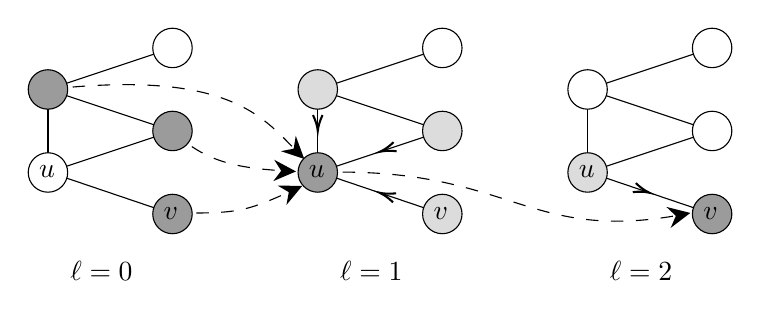
\begin{tikzpicture}[x=0.75pt,y=0.75pt,yscale=-1,xscale=1]
%uncomment if require: \path (0,160); %set diagram left start at 0, and has height of 160

%Curve Lines [id:da4313717085077018] 
\draw  [dash pattern={on 4.5pt off 4.5pt}]  (40.5,40.5) .. controls (128.99,30.61) and (144.66,54.47) .. (162.09,72.11) ;
\draw [shift={(164,74)}, rotate = 224.13] [fill={rgb, 255:red, 0; green, 0; blue, 0 }  ][line width=0.08]  [draw opacity=0] (10.72,-5.15) -- (0,0) -- (10.72,5.15) -- (7.12,0) -- cycle    ;
%Curve Lines [id:da6954216550236572] 
\draw  [dash pattern={on 4.5pt off 4.5pt}]  (100.5,60.5) .. controls (116.13,75.22) and (130.65,78.52) .. (157.08,79.86) ;
\draw [shift={(160,80)}, rotate = 182.53] [fill={rgb, 255:red, 0; green, 0; blue, 0 }  ][line width=0.08]  [draw opacity=0] (10.72,-5.15) -- (0,0) -- (10.72,5.15) -- (7.12,0) -- cycle    ;
%Curve Lines [id:da3347980352129689] 
\draw  [dash pattern={on 4.5pt off 4.5pt}]  (100,100) .. controls (132.69,100.24) and (135.08,99.78) .. (160.57,88.11) ;
\draw [shift={(163,87)}, rotate = 515.36] [fill={rgb, 255:red, 0; green, 0; blue, 0 }  ][line width=0.08]  [draw opacity=0] (10.72,-5.15) -- (0,0) -- (10.72,5.15) -- (7.12,0) -- cycle    ;
%Curve Lines [id:da07095702036161233] 
\draw  [dash pattern={on 4.5pt off 4.5pt}]  (170.5,80.5) .. controls (264.25,77.28) and (270.58,115.47) .. (347.64,100.47) ;
\draw [shift={(350,100)}, rotate = 528.4200000000001] [fill={rgb, 255:red, 0; green, 0; blue, 0 }  ][line width=0.08]  [draw opacity=0] (10.72,-5.15) -- (0,0) -- (10.72,5.15) -- (7.12,0) -- cycle    ;
%Straight Lines [id:da47912352597118213] 
\draw    (40.5,50) -- (40.5,71) ;
%Straight Lines [id:da9922159879153771] 
\draw    (40.5,40.5) -- (100.5,60.5) ;
%Straight Lines [id:da20693867709022928] 
\draw    (40.5,80.5) -- (100.5,60.5) ;
%Straight Lines [id:da12726884670105187] 
\draw    (40,80) -- (100.5,100.5) ;
%Straight Lines [id:da005529487369804631] 
\draw    (100.5,20.5) -- (40.5,40.5) ;
%Shape: Circle [id:dp12978240920475836] 
\draw  [fill={rgb, 255:red, 155; green, 155; blue, 155 }  ,fill opacity=1 ] (31,40.5) .. controls (31,35.25) and (35.25,31) .. (40.5,31) .. controls (45.75,31) and (50,35.25) .. (50,40.5) .. controls (50,45.75) and (45.75,50) .. (40.5,50) .. controls (35.25,50) and (31,45.75) .. (31,40.5) -- cycle ;
%Shape: Circle [id:dp44461896764010267] 
\draw  [fill={rgb, 255:red, 255; green, 255; blue, 255 }  ,fill opacity=1 ] (91,20.5) .. controls (91,15.25) and (95.25,11) .. (100.5,11) .. controls (105.75,11) and (110,15.25) .. (110,20.5) .. controls (110,25.75) and (105.75,30) .. (100.5,30) .. controls (95.25,30) and (91,25.75) .. (91,20.5) -- cycle ;
%Shape: Circle [id:dp8226342601300562] 
\draw  [fill={rgb, 255:red, 155; green, 155; blue, 155 }  ,fill opacity=1 ] (91,60.5) .. controls (91,55.25) and (95.25,51) .. (100.5,51) .. controls (105.75,51) and (110,55.25) .. (110,60.5) .. controls (110,65.75) and (105.75,70) .. (100.5,70) .. controls (95.25,70) and (91,65.75) .. (91,60.5) -- cycle ;
%Shape: Circle [id:dp9576590983310105] 
\draw  [fill={rgb, 255:red, 255; green, 255; blue, 255 }  ,fill opacity=1 ] (31,80.5) .. controls (31,75.25) and (35.25,71) .. (40.5,71) .. controls (45.75,71) and (50,75.25) .. (50,80.5) .. controls (50,85.75) and (45.75,90) .. (40.5,90) .. controls (35.25,90) and (31,85.75) .. (31,80.5) -- cycle ;
%Shape: Circle [id:dp6767076773328078] 
\draw  [fill={rgb, 255:red, 155; green, 155; blue, 155 }  ,fill opacity=1 ] (91,100.5) .. controls (91,95.25) and (95.25,91) .. (100.5,91) .. controls (105.75,91) and (110,95.25) .. (110,100.5) .. controls (110,105.75) and (105.75,110) .. (100.5,110) .. controls (95.25,110) and (91,105.75) .. (91,100.5) -- cycle ;
%Straight Lines [id:da3797310936600804] 
\draw    (170.5,50) -- (170.5,71) ;
\draw [shift={(170.5,60.5)}, rotate = 270] [color={rgb, 255:red, 0; green, 0; blue, 0 }  ][line width=0.75]    (7.65,-2.3) .. controls (4.86,-0.97) and (2.31,-0.21) .. (0,0) .. controls (2.31,0.21) and (4.86,0.98) .. (7.65,2.3)   ;
%Straight Lines [id:da39313117597338243] 
\draw    (170.5,40.5) -- (230.5,60.5) ;
%Straight Lines [id:da11909283508234703] 
\draw    (170.5,80.5) -- (230.5,60.5) ;
\draw [shift={(200.5,70.5)}, rotate = 341.57] [color={rgb, 255:red, 0; green, 0; blue, 0 }  ][line width=0.75]    (7.65,-2.3) .. controls (4.86,-0.97) and (2.31,-0.21) .. (0,0) .. controls (2.31,0.21) and (4.86,0.98) .. (7.65,2.3)   ;
%Straight Lines [id:da3511148855222339] 
\draw    (170,80) -- (230.5,100.5) ;
\draw [shift={(200.25,90.25)}, rotate = 18.72] [color={rgb, 255:red, 0; green, 0; blue, 0 }  ][line width=0.75]    (7.65,-2.3) .. controls (4.86,-0.97) and (2.31,-0.21) .. (0,0) .. controls (2.31,0.21) and (4.86,0.98) .. (7.65,2.3)   ;
%Straight Lines [id:da6106293032869707] 
\draw    (230.5,20.5) -- (170.5,40.5) ;
%Shape: Circle [id:dp4701031138690044] 
\draw  [fill={rgb, 255:red, 220; green, 220; blue, 220 }  ,fill opacity=1 ] (161,40.5) .. controls (161,35.25) and (165.25,31) .. (170.5,31) .. controls (175.75,31) and (180,35.25) .. (180,40.5) .. controls (180,45.75) and (175.75,50) .. (170.5,50) .. controls (165.25,50) and (161,45.75) .. (161,40.5) -- cycle ;
%Shape: Circle [id:dp5321807173132955] 
\draw  [fill={rgb, 255:red, 255; green, 255; blue, 255 }  ,fill opacity=1 ] (221,20.5) .. controls (221,15.25) and (225.25,11) .. (230.5,11) .. controls (235.75,11) and (240,15.25) .. (240,20.5) .. controls (240,25.75) and (235.75,30) .. (230.5,30) .. controls (225.25,30) and (221,25.75) .. (221,20.5) -- cycle ;
%Shape: Circle [id:dp554517566024453] 
\draw  [fill={rgb, 255:red, 220; green, 220; blue, 220 }  ,fill opacity=1 ] (221,60.5) .. controls (221,55.25) and (225.25,51) .. (230.5,51) .. controls (235.75,51) and (240,55.25) .. (240,60.5) .. controls (240,65.75) and (235.75,70) .. (230.5,70) .. controls (225.25,70) and (221,65.75) .. (221,60.5) -- cycle ;
%Shape: Circle [id:dp6234497550508977] 
\draw  [fill={rgb, 255:red, 155; green, 155; blue, 155 }  ,fill opacity=1 ] (161,80.5) .. controls (161,75.25) and (165.25,71) .. (170.5,71) .. controls (175.75,71) and (180,75.25) .. (180,80.5) .. controls (180,85.75) and (175.75,90) .. (170.5,90) .. controls (165.25,90) and (161,85.75) .. (161,80.5) -- cycle ;
%Shape: Circle [id:dp6481128593514689] 
\draw  [fill={rgb, 255:red, 220; green, 220; blue, 220 }  ,fill opacity=1 ] (221,100.5) .. controls (221,95.25) and (225.25,91) .. (230.5,91) .. controls (235.75,91) and (240,95.25) .. (240,100.5) .. controls (240,105.75) and (235.75,110) .. (230.5,110) .. controls (225.25,110) and (221,105.75) .. (221,100.5) -- cycle ;
%Straight Lines [id:da010045754906601312] 
\draw    (300.5,50) -- (300.5,71) ;
%Straight Lines [id:da9723039406561984] 
\draw    (300.5,40.5) -- (360.5,60.5) ;
%Straight Lines [id:da7207693173524592] 
\draw    (300.5,80.5) -- (360.5,60.5) ;
%Straight Lines [id:da047867810436508895] 
\draw    (300,80) -- (360.5,100.5) ;
\draw [shift={(330.25,90.25)}, rotate = 198.72] [color={rgb, 255:red, 0; green, 0; blue, 0 }  ][line width=0.75]    (7.65,-2.3) .. controls (4.86,-0.97) and (2.31,-0.21) .. (0,0) .. controls (2.31,0.21) and (4.86,0.98) .. (7.65,2.3)   ;
%Straight Lines [id:da13877434621766804] 
\draw    (360.5,20.5) -- (300.5,40.5) ;
%Shape: Circle [id:dp9753163859311793] 
\draw  [fill={rgb, 255:red, 255; green, 255; blue, 255 }  ,fill opacity=1 ] (291,40.5) .. controls (291,35.25) and (295.25,31) .. (300.5,31) .. controls (305.75,31) and (310,35.25) .. (310,40.5) .. controls (310,45.75) and (305.75,50) .. (300.5,50) .. controls (295.25,50) and (291,45.75) .. (291,40.5) -- cycle ;
%Shape: Circle [id:dp03916750111680778] 
\draw  [fill={rgb, 255:red, 255; green, 255; blue, 255 }  ,fill opacity=1 ] (351,20.5) .. controls (351,15.25) and (355.25,11) .. (360.5,11) .. controls (365.75,11) and (370,15.25) .. (370,20.5) .. controls (370,25.75) and (365.75,30) .. (360.5,30) .. controls (355.25,30) and (351,25.75) .. (351,20.5) -- cycle ;
%Shape: Circle [id:dp7074039311567142] 
\draw  [fill={rgb, 255:red, 255; green, 255; blue, 255 }  ,fill opacity=1 ] (351,60.5) .. controls (351,55.25) and (355.25,51) .. (360.5,51) .. controls (365.75,51) and (370,55.25) .. (370,60.5) .. controls (370,65.75) and (365.75,70) .. (360.5,70) .. controls (355.25,70) and (351,65.75) .. (351,60.5) -- cycle ;
%Shape: Circle [id:dp4904701423686293] 
\draw  [fill={rgb, 255:red, 220; green, 220; blue, 220 }  ,fill opacity=1 ] (291,80.5) .. controls (291,75.25) and (295.25,71) .. (300.5,71) .. controls (305.75,71) and (310,75.25) .. (310,80.5) .. controls (310,85.75) and (305.75,90) .. (300.5,90) .. controls (295.25,90) and (291,85.75) .. (291,80.5) -- cycle ;
%Shape: Circle [id:dp8890572986824241] 
\draw  [fill={rgb, 255:red, 155; green, 155; blue, 155 }  ,fill opacity=1 ] (351,100.5) .. controls (351,95.25) and (355.25,91) .. (360.5,91) .. controls (365.75,91) and (370,95.25) .. (370,100.5) .. controls (370,105.75) and (365.75,110) .. (360.5,110) .. controls (355.25,110) and (351,105.75) .. (351,100.5) -- cycle ;

% Text Node
\draw (355,96) node [anchor=north west][inner sep=0.75pt]    {$v$};
% Text Node
\draw (225,96) node [anchor=north west][inner sep=0.75pt]    {$v$};
% Text Node
\draw (95,96) node [anchor=north west][inner sep=0.75pt]    {$v$};
% Text Node
\draw (295,76) node [anchor=north west][inner sep=0.75pt]    {$u$};
% Text Node
\draw (165,76) node [anchor=north west][inner sep=0.75pt]    {$u$};
% Text Node
\draw (35,76) node [anchor=north west][inner sep=0.75pt]    {$u$};

% Text Node
\draw (50,122) node [anchor=north west][inner sep=0.75pt]    {$\ell =0$};
% Text Node
\draw (180,122) node [anchor=north west][inner sep=0.75pt]    {$\ell =1$};
% Text Node
\draw (310,122) node [anchor=north west][inner sep=0.75pt]    {$\ell =2$};


\end{tikzpicture}}
    \caption{Context diffusion through message passing. Directed edges represent messages (\eg from node $u$ to $v$ at iteration $\ell=2$). Dashed arrows represent the implicit contextual information received by a node (in dark gray) through the messages from its neighbors (in light gray). Focusing on node $v$, its context at iteration $\ell=2$ is composed all the dark gray nodes (including $v$ itself).}
    \label{fig:context-diffusion}
\end{figure*}
In the literature, we distinguish three different approaches by which iterative context diffusion is implemented in practice, which we describe in the following.

\subsubsection*{Recursive Approaches}
In the recursive approach to context diffusion, message passing is formulated as a dynamical system. In this case, the state transition function is recursive, meaning that $\EncTrans = \EncTrans^{(1)} = \EncTrans^{(2)} = \ldots = \EncTrans^{(\ell)}$. Practically speaking, the mutual dependencies between hidden states are modeled with a single recurrent layer, which is run indefinitely until convergence. Some well-known representatives of this paradigm are the Graph Neural Network \citep{scarselli2009gnn}, the Graph Echo State Network \citep{gallicchio2010graphesn}, and the more recent Fast and Deep Graph Neural Network \citep{gallicchio2020fastdeepgnn}. To ensure convergence, these approaches impose contractive dynamics on the state transition function. While the Graph Neural Network enforces such constraints in the (supervised) loss function, the other two inherit convergence from the contractivity of (untrained) reservoir dynamics. Another example is the Gated Graph Neural Network \citep{li2016gatedgnn}, where, differently from \citet{scarselli2009gnn}, the number of iterations is fixed \apriori regardless of whether convergence is reached or not. Another approach based on \emph{collective inference}, which adopts the same strategy but does not rely on any particular convergence criteria, has been introduced in \citep{macskassy2007classificationnetworkdata}.

\subsubsection*{Feed-Forward Approaches}
The feed-forward approach is based on stacking multiple layers to compose the local context learned at each message passing iteration. As a result, the mutual dependencies between the hidden states are handled separately via differently parameterized layers, without the need of constraints to ensure the convergence of the state transition function. In practice, the state transition function is no more recursive, but changes at every layer. Thus, in the feed-forward case, the symbol $\ell$ indicates the layer that handles the corresponding message passing iteration. The effectiveness of the compositionality induced by the introduction of layers has been demonstrated in \citep{micheli2009nn4g}, where it is shown formally that the context of a node increases as a function of the network depth, up to including all the nodes in the graph. Feed-forward approaches are nowadays the main paradigm to design \glspl{dgn}, due to their simplicity, efficiency, and performance on different tasks. However, deep networks for graphs suffer from the same gradient-related problems as other deep \glspl{nn}, especially when associated with an end-to-end learning process running through the whole architecture \citep{bengio1994learninglongtermdependenciesdifficult,li2018deeperinsightgraphconvsemisupervised}. For the rest of this thesis, all the \glspl{dgn} used shall be feed-forward.

\subsubsection*{Constructive Approaches}
Constructive approaches are a special case of feed-forward models, in which training is performed layer-wise. The neural network architecture exploited by these models is a modification of the Cascade Correlation algorithm \citep{fahlman1990cascor} for graphs. The major benefit of constructive architectures is that deep networks do not incur the vanishing/exploding gradient problem by design. In supervised scenarios, the constructive technique can learn the number of layers needed to solve a task \citep{marquez2018deepcascade,bianucci2000cascorchemistry}. In other words, constructive \glspl{dgn} can determine automatically how much context is most beneficial to perform well, according to the specific task at hand. Another feature of constructive models is that they solve a problem in a \emph{divide-et-impera} fashion, rather than using end-to-end training, by incrementally splitting the task into manageable sub-tasks. Each layer solves its own sub-problem, and subsequent layers use their results to improve further on their own, addressing the global task progressively. Among the constructive approaches, we mention the Neural Network for Graphs \citep{micheli2009nn4g}, which was the first to propose a feed-forward architecture for graphs. Among recent models, another related approach which tackles the problem from a probabilistic point of view is the Contextual Graph Markov Model \citep{bacciu2018contgraphmarkov}.

\subsection{Building Blocks of Deep Graph Networks}
\glspl{dgn} are built from several architectural components, which we cover in detail in this section. In short, a supervised \gls{dgn} can be decomposed into a collection of layers that process the graph structure, and a downstream predictor (either a classifier or a regressor) that computes a task-dependent output using the representation obtained by the graph processing layers. The whole network is trained in an end-to-end fashion. In this section, we focus on the former components, the ones whose role is to carry out the processing of an input graph.

\subsubsection*{Graph Convolutional Layers}\label{sec:graph-conv-layers}
A \gls{gcl} is essentially a neural network layer that performs message passing. The term \quotes{convolutional} is used to remark that the local processing performed by the state transition function is a generalization of the convolutional layer for images to graph domains with variable-size neighborhoods. Given an attributed graph $\AttrGraph{g}$ with $n$ nodes, and its node attributes $\GraphFeatures{x}{g} = \Set{\Elem{x}{v} \in \Real^d \mid v \in \Nodes{g}}$, one general formulation of a \gls{gcl} is the following:
\begin{align}
    \label{eq:simple-aggregation}
    \StateVector{v}{\ell} = U \Par{\StateVector{v}{\ell-1}, A\Par{\Set{\,T(\StateVector{u}{\ell-1}) \mid u \in \Neigh(v)}}}, \; \forall v \in \Nodes{g},
\end{align}
where $\StateVector{v}{\ell} \in \Real^{h_\ell}$ is the hidden state of the node at layer $\ell$, $\,\StateVector{v}{\ell-1} \in \Real^{h_{\ell-1}}$ is the hidden state of the node at the previous layer $\ell-1$, and by convention $\StateVector{v}{0} = \Elem{x}{v}$. Notice that the neighborhood function $\Neigh$ is also implicitly passed as input of the layer, so that the connectivity of each node is known. We can identify three key functions inside a \gls{gcl}:
\begin{itemize}
    \item $T: \Real^{h_{\ell-1}} \shortrightarrow \Real^{h_{\ell-1}}$ is a \emph{transform} function that applies some transformation to the hidden states of neighbors of node $v$ at layer $\ell-1$. This can be any function, either fixed or adaptive (implemented by a neural network);
    \item $A: (\Real^{h_{\ell-1}} \times \Real^{h_{\ell-1}} \times \ldots) \shortrightarrow \Real^{h_{\ell-1}}$ is an \emph{aggregation} function that maps a \emph{multiset}\footnote{Given a set $\Cal{B}$, a multiset $\Multiset(\Cal{B})$ is a tuple $\Tuple{\Cal{B}, \varrho}$ where $\varrho: \Cal{B} \shortrightarrow \Natural_+$ gives the multiplicity of each element in $\Cal{B}$.} of transformed neighbors of $v$ to a unique \emph{neighborhood state vector}. In practice, $A$ is a \emph{permutation invariant} function, meaning that its output does not change upon reordering of the arguments. For this reason, the computation of the neighborhood state vector is often referred to as \emph{neighborhood aggregation};
    \item $U: (\Real^{h_{\ell-1}} \times \Real^{h_{\ell-1}}) \shortrightarrow \Real^{h_{\ell}}$ is an \emph{update} function that takes the hidden state of a node at layer $\ell-1$ and the aggregated vector, and combines them to produce the new hidden state of the node at layer $\ell$. Similarly to $T$, $U$ can also be fixed or adaptive.
\end{itemize}
The usage of a permutation invariant function to compute the state of the neighbors is crucial, as it allows acquiring information from nearby nodes in a non-positional fashion, which is often the case with real-world graphs. From this general formulation, several implementations can be realized. As an example, we report the well-known formulation of \citet{kipf2017semisupervisedgcn}, corresponding to the \gls{gcn} model:
\begin{align}
    \label{eq:convolutional}
    \StateVector{v}{\ell} = \sigmoid\Par{ \LayerMatrix{w}{\ell} \sum_{u \in \Neigh(v)} \tilde{l}_{uv}\StateVector{u}{\ell-1}}, \; \forall v \in \Nodes{g},
\end{align}
where $\tilde{l}_{uv}$ is the entry of the symmetric normalized graph Laplacian $\NormLaplacianMatrix{g}$ related to nodes $u$ and $v$, and:
\begin{align}
    \label{eq:transform}
    T(\StateVector{u}{\ell-1}) &= \GenStateVector{t}{v}{\ell-1}  = \tilde{l}_{uv}\,\StateVector{u}{\ell-1}\\
    \label{eq:aggregate}
    A\Par{\Set{\GenStateVector{t}{v}{\ell-1} \mid u \in \Neigh(v)}} &= \GenStateVector{n}{v}{\ell-1} = \sum_{u \in \Neigh(v)} \GenStateVector{t}{v}{\ell-1}\\
    \label{eq:update}
    U(\StateVector{v}{\ell-1}, \GenStateVector{n}{v}{\ell-1}) &= \StateVector{v}{\ell} =  \sigmoid\Par{\LayerMatrix{w}{\ell}\, \GenStateVector{n}{v}{\ell-1}}.
\end{align}
In this case, the aggregation function is the sum function. Other examples of permutation invariant functions used in practical contexts are the mean, the max, or other general functions which work on multisets \citep{zaheer2017deepsets}. Notice that a \gls{gcl} can be applied simultaneously to all the nodes in the graph, corresponding to visiting the graph nodes in parallel, with no predefined ordering. This contrasts with \glspl{rnn} and \glspl{recnn}, where parallelism in the state calculations is not possible or limited, respectively.

The generic \gls{gcl} can be rewritten in matrix form as some variation of the following:
$$\LayerStateMat{\ell} = \Fun{GCL}(\AdjMatrix{g}, \LayerStateMat{\ell-1}) =   \sigma\Par{\AdjMatrix{g}\LayerStateMat{\ell-1}\LayerMatrix{w}{\ell}} \in \Real^{n \times h^{(\ell)}},$$
where $\AdjMatrix{g} \in \Real^{n \times n}$ is the adjacency matrix of the graph, $\LayerStateMat{\ell-1} \in \Real^{n \times h}$ are the hidden states computed at layer $\ell-1$ where by convention $\LayerStateMat{0} = \FeatureMatrix{g} \in \Real^{n \times d}$ is the matrix of node features, and $\LayerMatrix{w}{\ell} \in \Real^{h_{(\ell-1)} \times h_{(\ell)}}$ is the matrix of trainable layer-wise weights. Here, the adjacency matrix substitutes the neighborhood function $\Neigh$, and the adjacency sets are inferred by its rows and columns. With this formulation, the \gls{gcl} can be vectorized, which allows to run the state computation in fast hardware such as \glspl{gpu}.

\paragraph{Handling Edges}
In certain tasks, including information about the edge features to the message passing algorithm can be beneficial to performances. Here, we describe how this can be achieved, focusing on the case where the edge features are discrete values out of a set of $K$ possible choices. Specifically, given an attributed graph $\AttrGraph{g}$, we assume a set of edge features of the form $\GraphFeatures{e}{g} = \Set{\Elem{e}{u,v} \in \Cal{C} \mid (u, v) \in \Edges{g}}$, with $\Cal{C} = \Set{c_i}_{i=1}^K$. To account for different edge types, two modifications to the message passing algorithm are required. One is to replace the standard neighborhood function in the aggregation function with the following \emph{edge-aware} neighborhood function of a node $v$:
$$\Neigh_c(v) = \Set{u \in \Neigh(v) \mid \Indicator{\Elem{e}{u, v} = c}},$$
which selects only neighbors of $v$ with edge type $c$. The other modification requires to change the update function for handling the different edge types. Taking again the \gls{gcn} implementation as an example, Eq. \ref{eq:update} is modified as follows:
\begin{align*}
    \StateVector{v}{\ell} = \sigmoid\Par{\sum_{c \in \Cal{C}} \LayerMatrix{w}{\ell}_c \sum_{u \in \Neigh_c(v)} \tilde{l}_{uv}\,\Elem{h}{v}^{(\ell-1)}},\; \forall v \in \Nodes{g},
\end{align*}
where the weight matrices $\LayerMatrix{w}{\ell}_c $ are now edge-specific, so that the contributions of the different edge types are weighted adaptively \citep{micheli2009nn4g,schlichtkrull2018relationaldatagcn}. In practice, the above procedure corresponds to performing $K$ different aggregations weighted separately to compute the state of the node. Other approaches to include edge information in the message passing scheme require to extend the transform function, such that the edges between the processed node and its neighbors are included in the transformation (for example, by concatenating the edge feature to the hidden state vector) \cite{gilmer2017neuralmessagepassing}.

\paragraph{Node Attention}
Attention mechanisms \citep{bahdanau2015attention} are a widely used tool in Deep Learning to get importance scores out of arbitrary sets of items. Thus, they are naturally applicable within the \gls{dgn} framework to measure the contribution of the different nodes during neighborhood aggregation. Specifically, to introduce attention mechanisms in the neighborhood aggregation, the contribution of the transformed nodes in the neighborhood is weighted by a scalar $a^{(\ell)}_{uv} \in \Real$, called \emph{attention score} as follows:
$$A(\Set{\,a^{(\ell)}_{uv}\,T(\StateVector{u}{\ell-1}) \mid u \in \Neigh(v)}).$$
The attention scores are derived from \emph{attention coefficients} $w_{vu}^{(\ell)}$, which are essentially similarity scores between the neighbor and the current node, calculated as follows:
$$w_{vu}^{(\ell)} = f(\StateVector{v}{\ell}, \StateVector{u}{\ell}),$$
where $f$ is an arbitrary neural network. Different attention mechanisms are defined based on how $f$ is implemented (\eg in the Graph Attention Network \cite{velickovic2018gat}, the two states are concatenated). Finally, the coefficients are normalized into attention scores by a softmax function, effectively defining a probability distribution among them. The attention mechanism can be generalized to \emph{multi-head} attention, where multiple attention scores for each node are calculated and concatenated together to obtain an attention vector, rather than a score. Figure \ref{fig:attention} shows an example of attention computed on an example graph. We remark that node attention is unrelated to weighting the connection between nodes, which is an operation that involves the edge features. Here, similarity between nodes is calculated relying solely on the hidden states of the involved node and its neighbors.

\begin{figure*}[h!]
    \centering
    \resizebox{.35\textwidth}{!}{

\tikzset{every picture/.style={line width=0.75pt}} %set default line width to 0.75pt        

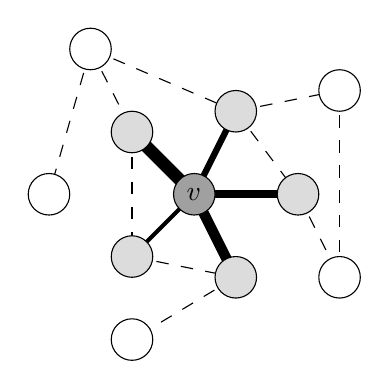
\begin{tikzpicture}[x=0.75pt,y=0.75pt,yscale=-1,xscale=1]
%uncomment if require: \path (0,180); %set diagram left start at 0, and has height of 180

%Straight Lines [id:da5686945126074561] 
\draw [line width=4.5]    (110,55) -- (140,85) ;
%Straight Lines [id:da9604209522132989] 
\draw [line width=2.25]    (140,85) -- (160,45) ;
%Straight Lines [id:da37557239319608837] 
\draw [line width=3]    (140,85) -- (190,85) ;
%Straight Lines [id:da6300189028004446] 
\draw [line width=3.75]    (140,85) -- (160,125) ;
%Straight Lines [id:da7961671100503147] 
\draw [line width=1.5]    (110,115) -- (140,85) ;
%Straight Lines [id:da3914617106414984] 
\draw  [dash pattern={on 4.5pt off 4.5pt}]  (110,55) -- (110,115) ;
%Straight Lines [id:da07988436759828788] 
\draw  [dash pattern={on 4.5pt off 4.5pt}]  (160,45) -- (190,85) ;
%Straight Lines [id:da7974028440726391] 
\draw  [dash pattern={on 4.5pt off 4.5pt}]  (190,85) -- (210,125) ;
%Straight Lines [id:da9163453027130692] 
\draw  [dash pattern={on 4.5pt off 4.5pt}]  (210,35) -- (210,125) ;
%Straight Lines [id:da8269233974334222] 
\draw  [dash pattern={on 4.5pt off 4.5pt}]  (160,45) -- (210,35) ;
%Straight Lines [id:da4638034672823643] 
\draw  [dash pattern={on 4.5pt off 4.5pt}]  (110,115) -- (160,125) ;
%Straight Lines [id:da8106142104727672] 
\draw  [dash pattern={on 4.5pt off 4.5pt}]  (160,125) -- (110,155) ;
%Straight Lines [id:da18520110140050194] 
\draw  [dash pattern={on 4.5pt off 4.5pt}]  (90,15) -- (70,85) ;
%Straight Lines [id:da625081015703862] 
\draw  [dash pattern={on 4.5pt off 4.5pt}]  (90,15) -- (160,45) ;
%Straight Lines [id:da82285820802776] 
\draw  [dash pattern={on 4.5pt off 4.5pt}]  (90,15) -- (111.24,56.72) ;
%Shape: Circle [id:dp9141923177042026] 
\draw  [fill={rgb, 255:red, 160; green, 160; blue, 160 }  ,fill opacity=1 ] (130,85) .. controls (130,79.48) and (134.48,75) .. (140,75) .. controls (145.52,75) and (150,79.48) .. (150,85) .. controls (150,90.52) and (145.52,95) .. (140,95) .. controls (134.48,95) and (130,90.52) .. (130,85) -- cycle ;
%Shape: Circle [id:dp18272847458947417] 
\draw  [fill={rgb, 255:red, 220; green, 220; blue, 220 }  ,fill opacity=1 ] (150,45) .. controls (150,39.48) and (154.48,35) .. (160,35) .. controls (165.52,35) and (170,39.48) .. (170,45) .. controls (170,50.52) and (165.52,55) .. (160,55) .. controls (154.48,55) and (150,50.52) .. (150,45) -- cycle ;
%Shape: Circle [id:dp6485883310805953] 
\draw  [fill={rgb, 255:red, 220; green, 220; blue, 220 }  ,fill opacity=1 ] (180,85) .. controls (180,79.48) and (184.48,75) .. (190,75) .. controls (195.52,75) and (200,79.48) .. (200,85) .. controls (200,90.52) and (195.52,95) .. (190,95) .. controls (184.48,95) and (180,90.52) .. (180,85) -- cycle ;
%Shape: Circle [id:dp4567157214251971] 
\draw  [fill={rgb, 255:red, 220; green, 220; blue, 220 }  ,fill opacity=1 ] (150,125) .. controls (150,119.48) and (154.48,115) .. (160,115) .. controls (165.52,115) and (170,119.48) .. (170,125) .. controls (170,130.52) and (165.52,135) .. (160,135) .. controls (154.48,135) and (150,130.52) .. (150,125) -- cycle ;
%Shape: Circle [id:dp9772039662669827] 
\draw  [fill={rgb, 255:red, 220; green, 220; blue, 220 }  ,fill opacity=1 ] (100,115) .. controls (100,109.48) and (104.48,105) .. (110,105) .. controls (115.52,105) and (120,109.48) .. (120,115) .. controls (120,120.52) and (115.52,125) .. (110,125) .. controls (104.48,125) and (100,120.52) .. (100,115) -- cycle ;
%Shape: Circle [id:dp849968227587317] 
\draw  [fill={rgb, 255:red, 220; green, 220; blue, 220 }  ,fill opacity=1 ] (100,55) .. controls (100,49.48) and (104.48,45) .. (110,45) .. controls (115.52,45) and (120,49.48) .. (120,55) .. controls (120,60.52) and (115.52,65) .. (110,65) .. controls (104.48,65) and (100,60.52) .. (100,55) -- cycle ;
%Shape: Circle [id:dp3852456165614402] 
\draw  [fill={rgb, 255:red, 255; green, 255; blue, 255 }  ,fill opacity=1 ] (60,85) .. controls (60,79.48) and (64.48,75) .. (70,75) .. controls (75.52,75) and (80,79.48) .. (80,85) .. controls (80,90.52) and (75.52,95) .. (70,95) .. controls (64.48,95) and (60,90.52) .. (60,85) -- cycle ;
%Shape: Circle [id:dp2002495564114657] 
\draw  [fill={rgb, 255:red, 255; green, 255; blue, 255 }  ,fill opacity=1 ] (80,15) .. controls (80,9.48) and (84.48,5) .. (90,5) .. controls (95.52,5) and (100,9.48) .. (100,15) .. controls (100,20.52) and (95.52,25) .. (90,25) .. controls (84.48,25) and (80,20.52) .. (80,15) -- cycle ;
%Shape: Circle [id:dp11701891156215805] 
\draw  [fill={rgb, 255:red, 255; green, 255; blue, 255 }  ,fill opacity=1 ] (200,35) .. controls (200,29.48) and (204.48,25) .. (210,25) .. controls (215.52,25) and (220,29.48) .. (220,35) .. controls (220,40.52) and (215.52,45) .. (210,45) .. controls (204.48,45) and (200,40.52) .. (200,35) -- cycle ;
%Shape: Circle [id:dp7052954164459615] 
\draw  [fill={rgb, 255:red, 255; green, 255; blue, 255 }  ,fill opacity=1 ] (200,125) .. controls (200,119.48) and (204.48,115) .. (210,115) .. controls (215.52,115) and (220,119.48) .. (220,125) .. controls (220,130.52) and (215.52,135) .. (210,135) .. controls (204.48,135) and (200,130.52) .. (200,125) -- cycle ;
%Shape: Circle [id:dp9425951388234] 
\draw  [fill={rgb, 255:red, 255; green, 255; blue, 255 }  ,fill opacity=1 ] (100,155) .. controls (100,149.48) and (104.48,145) .. (110,145) .. controls (115.52,145) and (120,149.48) .. (120,155) .. controls (120,160.52) and (115.52,165) .. (110,165) .. controls (104.48,165) and (100,160.52) .. (100,155) -- cycle ;

% Text Node
\draw (135,81) node [anchor=north west][inner sep=0.75pt]    {$v$};


\end{tikzpicture}}
    \caption{An example of node attention. Edge thicknesses are not related to the strength of the connection between node $v$ (in dark gray) and its neighbors (in light gray), but it represents the degree of similarity between the node states, quantified in a probabilistic sense by the attention score. Dashed edges connect nodes that are not involved in the attention score computation.}
    \label{fig:attention}
\end{figure*}

\paragraph{Node Sampling}
Node sampling is a technique used when learning on large graphs to ensure computational efficiency. When the number of nodes in a graph is large, and nodes are densely connected among themselves, computing neighborhood aggregation may become very expensive or even intractable. The most straightforward method to address this issue is to randomly sample a predefined number of nodes to aggregate, rather than using the whole neighborhood. This basic strategy can be refined by using more sophisticated techniques such as importance sampling \citep{gallicchio2020fastdeepgnn}, or even extended to sampling a bounded number of nodes which are not necessarily in the immediate neighborhood of the current node \citep{hamilton2017graphsage}. The latter requires adding fictitious edges between the current node and nodes at farther distances, in order to treat them as standard neighbors. This way, global information about the graph can be incorporated more directly, as compared to message passing.

\begin{figure*}[h!]
    \centering
    \resizebox{.35\textwidth}{!}{

\tikzset{every picture/.style={line width=0.75pt}} %set default line width to 0.75pt        

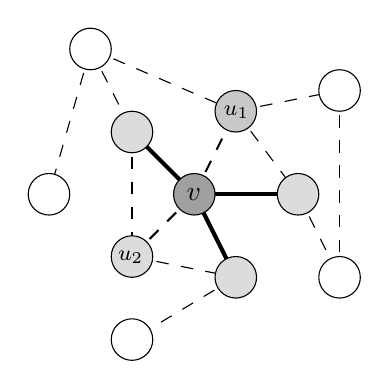
\begin{tikzpicture}[x=0.75pt,y=0.75pt,yscale=-1,xscale=1]
%uncomment if require: \path (0,180); %set diagram left start at 0, and has height of 180

%Straight Lines [id:da9928972582367306] 
\draw [line width=1.5]    (110,55) -- (140,85) ;
%Straight Lines [id:da7590045228035791] 
\draw [line width=0.75]  [dash pattern={on 4.5pt off 4.5pt}]  (140,85) -- (160,45) ;
%Straight Lines [id:da9311764026080076] 
\draw [line width=1.5]    (140,85) -- (190,85) ;
%Straight Lines [id:da7051144357210035] 
\draw [line width=1.5]    (140,85) -- (160,125) ;
%Straight Lines [id:da9499976233652532] 
\draw [line width=0.75]  [dash pattern={on 4.5pt off 4.5pt}]  (110,115) -- (140,85) ;
%Straight Lines [id:da6071610287175291] 
\draw  [dash pattern={on 4.5pt off 4.5pt}]  (110,55) -- (110,115) ;
%Straight Lines [id:da458862675888432] 
\draw  [dash pattern={on 4.5pt off 4.5pt}]  (160,45) -- (190,85) ;
%Straight Lines [id:da03442786949532706] 
\draw  [dash pattern={on 4.5pt off 4.5pt}]  (190,85) -- (210,125) ;
%Straight Lines [id:da1577597063925078] 
\draw  [dash pattern={on 4.5pt off 4.5pt}]  (210,35) -- (210,125) ;
%Straight Lines [id:da4513425022479223] 
\draw  [dash pattern={on 4.5pt off 4.5pt}]  (160,45) -- (210,35) ;
%Straight Lines [id:da9391313397847703] 
\draw  [dash pattern={on 4.5pt off 4.5pt}]  (110,115) -- (160,125) ;
%Straight Lines [id:da1766664603992849] 
\draw  [dash pattern={on 4.5pt off 4.5pt}]  (160,125) -- (110,155) ;
%Straight Lines [id:da38513478626684483] 
\draw  [dash pattern={on 4.5pt off 4.5pt}]  (90,15) -- (70,85) ;
%Straight Lines [id:da5306220988073596] 
\draw  [dash pattern={on 4.5pt off 4.5pt}]  (90,15) -- (160,45) ;
%Straight Lines [id:da6886418274825212] 
\draw  [dash pattern={on 4.5pt off 4.5pt}]  (90,15) -- (111.24,56.72) ;
%Shape: Circle [id:dp771344607660861] 
\draw  [fill={rgb, 255:red, 160; green, 160; blue, 160 }  ,fill opacity=1 ] (130,85) .. controls (130,79.48) and (134.48,75) .. (140,75) .. controls (145.52,75) and (150,79.48) .. (150,85) .. controls (150,90.52) and (145.52,95) .. (140,95) .. controls (134.48,95) and (130,90.52) .. (130,85) -- cycle ;
%Shape: Circle [id:dp27537395956973] 
\draw  [fill={rgb, 255:red, 200; green, 200; blue, 200 }  ,fill opacity=1 ] (150,45) .. controls (150,39.48) and (154.48,35) .. (160,35) .. controls (165.52,35) and (170,39.48) .. (170,45) .. controls (170,50.52) and (165.52,55) .. (160,55) .. controls (154.48,55) and (150,50.52) .. (150,45) -- cycle ;
%Shape: Circle [id:dp9311025651782232] 
\draw  [fill={rgb, 255:red, 220; green, 220; blue, 220 }  ,fill opacity=1 ] (180,85) .. controls (180,79.48) and (184.48,75) .. (190,75) .. controls (195.52,75) and (200,79.48) .. (200,85) .. controls (200,90.52) and (195.52,95) .. (190,95) .. controls (184.48,95) and (180,90.52) .. (180,85) -- cycle ;
%Shape: Circle [id:dp3681889727661305] 
\draw  [fill={rgb, 255:red, 220; green, 220; blue, 220 }  ,fill opacity=1 ] (150,125) .. controls (150,119.48) and (154.48,115) .. (160,115) .. controls (165.52,115) and (170,119.48) .. (170,125) .. controls (170,130.52) and (165.52,135) .. (160,135) .. controls (154.48,135) and (150,130.52) .. (150,125) -- cycle ;
%Shape: Circle [id:dp4411140386684782] 
\draw  [fill={rgb, 255:red, 220; green, 220; blue, 220 }  ,fill opacity=1 ] (100,115) .. controls (100,109.48) and (104.48,105) .. (110,105) .. controls (115.52,105) and (120,109.48) .. (120,115) .. controls (120,120.52) and (115.52,125) .. (110,125) .. controls (104.48,125) and (100,120.52) .. (100,115) -- cycle ;
%Shape: Circle [id:dp22700882921378018] 
\draw  [fill={rgb, 255:red, 220; green, 220; blue, 220 }  ,fill opacity=1 ] (100,55) .. controls (100,49.48) and (104.48,45) .. (110,45) .. controls (115.52,45) and (120,49.48) .. (120,55) .. controls (120,60.52) and (115.52,65) .. (110,65) .. controls (104.48,65) and (100,60.52) .. (100,55) -- cycle ;
%Shape: Circle [id:dp1737413883891752] 
\draw  [fill={rgb, 255:red, 255; green, 255; blue, 255 }  ,fill opacity=1 ] (60,85) .. controls (60,79.48) and (64.48,75) .. (70,75) .. controls (75.52,75) and (80,79.48) .. (80,85) .. controls (80,90.52) and (75.52,95) .. (70,95) .. controls (64.48,95) and (60,90.52) .. (60,85) -- cycle ;
%Shape: Circle [id:dp9017509150985334] 
\draw  [fill={rgb, 255:red, 255; green, 255; blue, 255 }  ,fill opacity=1 ] (80,15) .. controls (80,9.48) and (84.48,5) .. (90,5) .. controls (95.52,5) and (100,9.48) .. (100,15) .. controls (100,20.52) and (95.52,25) .. (90,25) .. controls (84.48,25) and (80,20.52) .. (80,15) -- cycle ;
%Shape: Circle [id:dp1681742526969252] 
\draw  [fill={rgb, 255:red, 255; green, 255; blue, 255 }  ,fill opacity=1 ] (200,35) .. controls (200,29.48) and (204.48,25) .. (210,25) .. controls (215.52,25) and (220,29.48) .. (220,35) .. controls (220,40.52) and (215.52,45) .. (210,45) .. controls (204.48,45) and (200,40.52) .. (200,35) -- cycle ;
%Shape: Circle [id:dp32379455826600156] 
\draw  [fill={rgb, 255:red, 255; green, 255; blue, 255 }  ,fill opacity=1 ] (200,125) .. controls (200,119.48) and (204.48,115) .. (210,115) .. controls (215.52,115) and (220,119.48) .. (220,125) .. controls (220,130.52) and (215.52,135) .. (210,135) .. controls (204.48,135) and (200,130.52) .. (200,125) -- cycle ;
%Shape: Circle [id:dp8687072580412498] 
\draw  [fill={rgb, 255:red, 255; green, 255; blue, 255 }  ,fill opacity=1 ] (100,155) .. controls (100,149.48) and (104.48,145) .. (110,145) .. controls (115.52,145) and (120,149.48) .. (120,155) .. controls (120,160.52) and (115.52,165) .. (110,165) .. controls (104.48,165) and (100,160.52) .. (100,155) -- cycle ;

% Text Node
\draw (135,81) node [anchor=north west][inner sep=0.75pt]    {$v$};
% Text Node
\draw (153,41) node [anchor=north west][inner sep=0.75pt]  [font=\footnotesize]  {$u_{1}$};
% Text Node
\draw (102,111) node [anchor=north west][inner sep=0.75pt]  [font=\footnotesize]  {$u_{2}$};


\end{tikzpicture}}
    \caption{An example of node sampling. We focus on a node $v$ (in dark gray), and its neighbors (in light gray). Dashed edges connect nodes that are not involved in the neighborhood aggregation; notice how node $u$ is excluded, even though it is effectively a neighbor of $v$.}
    \label{fig:sampling}
\end{figure*}

\subsubsection*{Readout Layers}
As we have seen, the application of $L$ \gls{dgn} layers to an attributed graph $\AttrGraph{G}$ yields $L$ hidden states per node, each one composed with a progressively broad context. In node classification or regression tasks, these are combined by a \emph{hidden state readout} function to obtain a unique vector to use as input of the output function, which emits a prediction for every node. Specifically, a hidden state readout function $\Fun{R'}$ computes a \keyword{node representation} (or \keyword{node embedding}) $\StateVector{v}{*}$ for each node as follows:
$$\StateVector{v}{*} = \Op{R'}_{v}\Par{\Set{\StateVector{v}{\ell} \mid \ell = 1, \ldots, L}},\;  \forall v \in \Nodes{g}. $$
Notice that, when aggregating hidden states, one can exploit the fact that the number of layers is fixed beforehand in feed-forward \gls{dgn} architectures, and that the hidden states are ordered depth-wise. Thus, the layer-wise aggregations need not be permutation-invariant. Usual choices of $\Op{R'}_{v}$ include concatenation, weighted average (where the mixing weights can also be learned), \gls{rnn}s, or just selecting the hidden state at the last layer. The node representations are then fed to an output layer or downstream network, which computes node-wise outputs:
$$\Elem{o}{v} = g(\StateVector{v}{*}),\; \forall v \in \Nodes{g},$$
where $\Elem{o}{v} \in \Real^y$ and $g$ can be any arbitrarily complex neural network as usual. A visual example of the process for a single node is shown in Figure \ref{fig:node-readout}.
\begin{figure*}[h!]
    \centering
    \resizebox{.8\textwidth}{!}{

\tikzset{every picture/.style={line width=0.75pt}} %set default line width to 0.75pt        

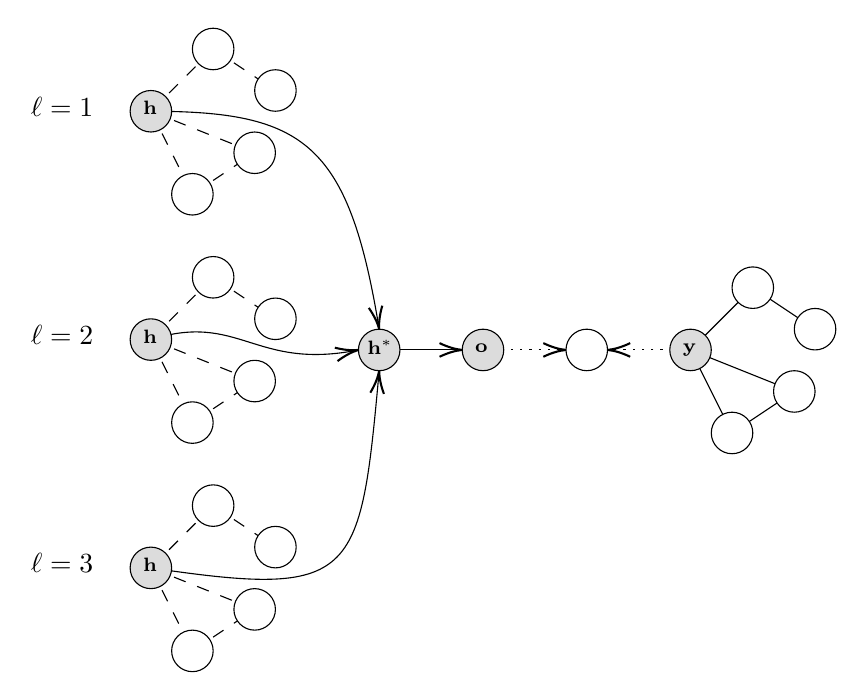
\begin{tikzpicture}[x=0.75pt,y=0.75pt,yscale=-1,xscale=1]
%uncomment if require: \path (0,325); %set diagram left start at 0, and has height of 325

%Straight Lines [id:da8021808052596502] 
\draw    (180,165) -- (218,165) ;
\draw [shift={(220,165)}, rotate = 180] [color={rgb, 255:red, 0; green, 0; blue, 0 }  ][line width=0.75]    (10.93,-3.29) .. controls (6.95,-1.4) and (3.31,-0.3) .. (0,0) .. controls (3.31,0.3) and (6.95,1.4) .. (10.93,3.29)   ;
%Straight Lines [id:da8262157575030338] 
\draw  [dash pattern={on 4.5pt off 4.5pt}]  (100,130) -- (70,160) ;
%Straight Lines [id:da09418463263497934] 
\draw  [dash pattern={on 4.5pt off 4.5pt}]  (70,160) -- (90,200) ;
%Straight Lines [id:da04169663842617122] 
\draw  [dash pattern={on 4.5pt off 4.5pt}]  (70,160) -- (120,180) ;
%Straight Lines [id:da9649034616072283] 
\draw  [dash pattern={on 4.5pt off 4.5pt}]  (90,200) -- (120,180) ;
%Straight Lines [id:da9180072651610127] 
\draw  [dash pattern={on 4.5pt off 4.5pt}]  (100,130) -- (130,150) ;
%Shape: Circle [id:dp5528328090096748] 
\draw  [fill={rgb, 255:red, 255; green, 255; blue, 255 }  ,fill opacity=1 ] (80,200) .. controls (80,194.48) and (84.48,190) .. (90,190) .. controls (95.52,190) and (100,194.48) .. (100,200) .. controls (100,205.52) and (95.52,210) .. (90,210) .. controls (84.48,210) and (80,205.52) .. (80,200) -- cycle ;
%Shape: Circle [id:dp9881598411642218] 
\draw  [fill={rgb, 255:red, 255; green, 255; blue, 255 }  ,fill opacity=1 ] (110,180) .. controls (110,174.48) and (114.48,170) .. (120,170) .. controls (125.52,170) and (130,174.48) .. (130,180) .. controls (130,185.52) and (125.52,190) .. (120,190) .. controls (114.48,190) and (110,185.52) .. (110,180) -- cycle ;
%Shape: Circle [id:dp8848288279392054] 
\draw  [fill={rgb, 255:red, 255; green, 255; blue, 255 }  ,fill opacity=1 ] (120,150) .. controls (120,144.48) and (124.48,140) .. (130,140) .. controls (135.52,140) and (140,144.48) .. (140,150) .. controls (140,155.52) and (135.52,160) .. (130,160) .. controls (124.48,160) and (120,155.52) .. (120,150) -- cycle ;
%Shape: Circle [id:dp4318188413506394] 
\draw  [fill={rgb, 255:red, 255; green, 255; blue, 255 }  ,fill opacity=1 ] (90,130) .. controls (90,124.48) and (94.48,120) .. (100,120) .. controls (105.52,120) and (110,124.48) .. (110,130) .. controls (110,135.52) and (105.52,140) .. (100,140) .. controls (94.48,140) and (90,135.52) .. (90,130) -- cycle ;
%Straight Lines [id:da45587472919699423] 
\draw  [dash pattern={on 4.5pt off 4.5pt}]  (100,20) -- (70,50) ;
%Straight Lines [id:da3322812526365526] 
\draw  [dash pattern={on 4.5pt off 4.5pt}]  (70,50) -- (90,90) ;
%Straight Lines [id:da060418746819522307] 
\draw  [dash pattern={on 4.5pt off 4.5pt}]  (70,50) -- (120,70) ;
%Straight Lines [id:da6519027932168682] 
\draw  [dash pattern={on 4.5pt off 4.5pt}]  (90,90) -- (120,70) ;
%Straight Lines [id:da10647901279823291] 
\draw  [dash pattern={on 4.5pt off 4.5pt}]  (100,20) -- (130,40) ;
%Shape: Circle [id:dp6069852564048885] 
\draw  [fill={rgb, 255:red, 255; green, 255; blue, 255 }  ,fill opacity=1 ] (80,90) .. controls (80,84.48) and (84.48,80) .. (90,80) .. controls (95.52,80) and (100,84.48) .. (100,90) .. controls (100,95.52) and (95.52,100) .. (90,100) .. controls (84.48,100) and (80,95.52) .. (80,90) -- cycle ;
%Shape: Circle [id:dp28187241585395206] 
\draw  [fill={rgb, 255:red, 255; green, 255; blue, 255 }  ,fill opacity=1 ] (110,70) .. controls (110,64.48) and (114.48,60) .. (120,60) .. controls (125.52,60) and (130,64.48) .. (130,70) .. controls (130,75.52) and (125.52,80) .. (120,80) .. controls (114.48,80) and (110,75.52) .. (110,70) -- cycle ;
%Shape: Circle [id:dp36091441623126763] 
\draw  [fill={rgb, 255:red, 255; green, 255; blue, 255 }  ,fill opacity=1 ] (120,40) .. controls (120,34.48) and (124.48,30) .. (130,30) .. controls (135.52,30) and (140,34.48) .. (140,40) .. controls (140,45.52) and (135.52,50) .. (130,50) .. controls (124.48,50) and (120,45.52) .. (120,40) -- cycle ;
%Shape: Circle [id:dp48327367752052597] 
\draw  [fill={rgb, 255:red, 255; green, 255; blue, 255 }  ,fill opacity=1 ] (90,20) .. controls (90,14.48) and (94.48,10) .. (100,10) .. controls (105.52,10) and (110,14.48) .. (110,20) .. controls (110,25.52) and (105.52,30) .. (100,30) .. controls (94.48,30) and (90,25.52) .. (90,20) -- cycle ;
%Straight Lines [id:da6727907472991814] 
\draw  [dash pattern={on 4.5pt off 4.5pt}]  (100,240) -- (70,270) ;
%Straight Lines [id:da4536448975686458] 
\draw  [dash pattern={on 4.5pt off 4.5pt}]  (70,270) -- (90,310) ;
%Straight Lines [id:da46318384192507667] 
\draw  [dash pattern={on 4.5pt off 4.5pt}]  (70,270) -- (120,290) ;
%Straight Lines [id:da26138928549207874] 
\draw  [dash pattern={on 4.5pt off 4.5pt}]  (90,310) -- (120,290) ;
%Straight Lines [id:da25645750289270874] 
\draw  [dash pattern={on 4.5pt off 4.5pt}]  (100,240) -- (130,260) ;
%Shape: Circle [id:dp29709464392681206] 
\draw  [fill={rgb, 255:red, 255; green, 255; blue, 255 }  ,fill opacity=1 ] (80,310) .. controls (80,304.48) and (84.48,300) .. (90,300) .. controls (95.52,300) and (100,304.48) .. (100,310) .. controls (100,315.52) and (95.52,320) .. (90,320) .. controls (84.48,320) and (80,315.52) .. (80,310) -- cycle ;
%Shape: Circle [id:dp5007793010043322] 
\draw  [fill={rgb, 255:red, 255; green, 255; blue, 255 }  ,fill opacity=1 ] (110,290) .. controls (110,284.48) and (114.48,280) .. (120,280) .. controls (125.52,280) and (130,284.48) .. (130,290) .. controls (130,295.52) and (125.52,300) .. (120,300) .. controls (114.48,300) and (110,295.52) .. (110,290) -- cycle ;
%Shape: Circle [id:dp7842479967392513] 
\draw  [fill={rgb, 255:red, 255; green, 255; blue, 255 }  ,fill opacity=1 ] (120,260) .. controls (120,254.48) and (124.48,250) .. (130,250) .. controls (135.52,250) and (140,254.48) .. (140,260) .. controls (140,265.52) and (135.52,270) .. (130,270) .. controls (124.48,270) and (120,265.52) .. (120,260) -- cycle ;
%Shape: Circle [id:dp08352653569945168] 
\draw  [fill={rgb, 255:red, 255; green, 255; blue, 255 }  ,fill opacity=1 ] (90,240) .. controls (90,234.48) and (94.48,230) .. (100,230) .. controls (105.52,230) and (110,234.48) .. (110,240) .. controls (110,245.52) and (105.52,250) .. (100,250) .. controls (94.48,250) and (90,245.52) .. (90,240) -- cycle ;
%Straight Lines [id:da08172279961172113] 
\draw    (360,135) -- (330,165) ;
%Straight Lines [id:da5964854301837534] 
\draw    (330,165) -- (350,205) ;
%Straight Lines [id:da705675390083226] 
\draw    (330,165) -- (380,185) ;
%Straight Lines [id:da657700600239705] 
\draw    (350,205) -- (380,185) ;
%Straight Lines [id:da3851868502745348] 
\draw    (360,135) -- (390,155) ;
%Shape: Circle [id:dp724750055071185] 
\draw  [fill={rgb, 255:red, 255; green, 255; blue, 255 }  ,fill opacity=1 ] (340,205) .. controls (340,199.48) and (344.48,195) .. (350,195) .. controls (355.52,195) and (360,199.48) .. (360,205) .. controls (360,210.52) and (355.52,215) .. (350,215) .. controls (344.48,215) and (340,210.52) .. (340,205) -- cycle ;
%Shape: Circle [id:dp45589554777220975] 
\draw  [fill={rgb, 255:red, 255; green, 255; blue, 255 }  ,fill opacity=1 ] (370,185) .. controls (370,179.48) and (374.48,175) .. (380,175) .. controls (385.52,175) and (390,179.48) .. (390,185) .. controls (390,190.52) and (385.52,195) .. (380,195) .. controls (374.48,195) and (370,190.52) .. (370,185) -- cycle ;
%Shape: Circle [id:dp8985548220725617] 
\draw  [fill={rgb, 255:red, 255; green, 255; blue, 255 }  ,fill opacity=1 ] (380,155) .. controls (380,149.48) and (384.48,145) .. (390,145) .. controls (395.52,145) and (400,149.48) .. (400,155) .. controls (400,160.52) and (395.52,165) .. (390,165) .. controls (384.48,165) and (380,160.52) .. (380,155) -- cycle ;
%Shape: Circle [id:dp5150110802600167] 
\draw  [fill={rgb, 255:red, 255; green, 255; blue, 255 }  ,fill opacity=1 ] (350,135) .. controls (350,129.48) and (354.48,125) .. (360,125) .. controls (365.52,125) and (370,129.48) .. (370,135) .. controls (370,140.52) and (365.52,145) .. (360,145) .. controls (354.48,145) and (350,140.52) .. (350,135) -- cycle ;
%Curve Lines [id:da6191074648732291] 
\draw    (70,50) .. controls (143.43,50.05) and (165.08,64.9) .. (179.78,153.66) ;
\draw [shift={(180,155)}, rotate = 260.72] [color={rgb, 255:red, 0; green, 0; blue, 0 }  ][line width=0.75]    (10.93,-3.29) .. controls (6.95,-1.4) and (3.31,-0.3) .. (0,0) .. controls (3.31,0.3) and (6.95,1.4) .. (10.93,3.29)   ;
%Curve Lines [id:da12167346141027413] 
\draw    (70,160) .. controls (112.37,146.68) and (119.66,174.48) .. (168.51,165.29) ;
\draw [shift={(170,165)}, rotate = 528.6800000000001] [color={rgb, 255:red, 0; green, 0; blue, 0 }  ][line width=0.75]    (10.93,-3.29) .. controls (6.95,-1.4) and (3.31,-0.3) .. (0,0) .. controls (3.31,0.3) and (6.95,1.4) .. (10.93,3.29)   ;
%Curve Lines [id:da6495417615361903] 
\draw    (70,270) .. controls (168.8,284.68) and (170.78,275.34) .. (179.86,176.5) ;
\draw [shift={(180,175)}, rotate = 455.24] [color={rgb, 255:red, 0; green, 0; blue, 0 }  ][line width=0.75]    (10.93,-3.29) .. controls (6.95,-1.4) and (3.31,-0.3) .. (0,0) .. controls (3.31,0.3) and (6.95,1.4) .. (10.93,3.29)   ;
%Shape: Circle [id:dp8473323519447842] 
\draw  [fill={rgb, 255:red, 220; green, 220; blue, 220 }  ,fill opacity=1 ] (60,160) .. controls (60,154.48) and (64.48,150) .. (70,150) .. controls (75.52,150) and (80,154.48) .. (80,160) .. controls (80,165.52) and (75.52,170) .. (70,170) .. controls (64.48,170) and (60,165.52) .. (60,160) -- cycle ;
%Shape: Circle [id:dp877285523901683] 
\draw  [fill={rgb, 255:red, 220; green, 220; blue, 220 }  ,fill opacity=1 ] (60,50) .. controls (60,44.48) and (64.48,40) .. (70,40) .. controls (75.52,40) and (80,44.48) .. (80,50) .. controls (80,55.52) and (75.52,60) .. (70,60) .. controls (64.48,60) and (60,55.52) .. (60,50) -- cycle ;
%Shape: Circle [id:dp5471945476486635] 
\draw  [fill={rgb, 255:red, 220; green, 220; blue, 220 }  ,fill opacity=1 ] (60,270) .. controls (60,264.48) and (64.48,260) .. (70,260) .. controls (75.52,260) and (80,264.48) .. (80,270) .. controls (80,275.52) and (75.52,280) .. (70,280) .. controls (64.48,280) and (60,275.52) .. (60,270) -- cycle ;
%Straight Lines [id:da5747740801523578] 
\draw  [dash pattern={on 0.84pt off 2.51pt}]  (230,165) -- (268,165) ;
\draw [shift={(270,165)}, rotate = 180] [color={rgb, 255:red, 0; green, 0; blue, 0 }  ][line width=0.75]    (10.93,-3.29) .. controls (6.95,-1.4) and (3.31,-0.3) .. (0,0) .. controls (3.31,0.3) and (6.95,1.4) .. (10.93,3.29)   ;
%Straight Lines [id:da7736106844919413] 
\draw  [dash pattern={on 0.84pt off 2.51pt}]  (330,165) -- (292,165) ;
\draw [shift={(290,165)}, rotate = 360] [color={rgb, 255:red, 0; green, 0; blue, 0 }  ][line width=0.75]    (10.93,-3.29) .. controls (6.95,-1.4) and (3.31,-0.3) .. (0,0) .. controls (3.31,0.3) and (6.95,1.4) .. (10.93,3.29)   ;
%Shape: Circle [id:dp8719481497855568] 
\draw  [fill={rgb, 255:red, 220; green, 220; blue, 220 }  ,fill opacity=1 ] (170,165) .. controls (170,159.48) and (174.48,155) .. (180,155) .. controls (185.52,155) and (190,159.48) .. (190,165) .. controls (190,170.52) and (185.52,175) .. (180,175) .. controls (174.48,175) and (170,170.52) .. (170,165) -- cycle ;
%Shape: Circle [id:dp3225900460836928] 
\draw  [fill={rgb, 255:red, 255; green, 255; blue, 255 }  ,fill opacity=1 ] (270,165) .. controls (270,159.48) and (274.48,155) .. (280,155) .. controls (285.52,155) and (290,159.48) .. (290,165) .. controls (290,170.52) and (285.52,175) .. (280,175) .. controls (274.48,175) and (270,170.52) .. (270,165) -- cycle ;
%Shape: Circle [id:dp7781672542643503] 
\draw  [fill={rgb, 255:red, 220; green, 220; blue, 220 }  ,fill opacity=1 ] (320,165) .. controls (320,159.48) and (324.48,155) .. (330,155) .. controls (335.52,155) and (340,159.48) .. (340,165) .. controls (340,170.52) and (335.52,175) .. (330,175) .. controls (324.48,175) and (320,170.52) .. (320,165) -- cycle ;
%Shape: Circle [id:dp1531568176441671] 
\draw  [fill={rgb, 255:red, 220; green, 220; blue, 220 }  ,fill opacity=1 ] (220,165) .. controls (220,159.48) and (224.48,155) .. (230,155) .. controls (235.52,155) and (240,159.48) .. (240,165) .. controls (240,170.52) and (235.52,175) .. (230,175) .. controls (224.48,175) and (220,170.52) .. (220,165) -- cycle ;


% Text Node
\draw (273,160) node [anchor=north west][inner sep=0.75pt]  [font=\scriptsize]  {$\Loss$};
% Text Node
\draw (10.9,151.8) node [anchor=north west][inner sep=0.75pt]    {$\ell =2$};
% Text Node
\draw (10.9,261.8) node [anchor=north west][inner sep=0.75pt]    {$\ell =3$};
% Text Node
\draw (10.9,41.8) node [anchor=north west][inner sep=0.75pt]    {$\ell =1$};
% Text Node
\draw (65,44) node [anchor=north west][inner sep=0.75pt]  [font=\scriptsize]  {$\mathbf{h}$};
% Text Node
\draw (65,154) node [anchor=north west][inner sep=0.75pt]  [font=\scriptsize]  {$\mathbf{h}$};
% Text Node
\draw (65,264) node [anchor=north west][inner sep=0.75pt]  [font=\scriptsize]  {$\mathbf{h}$};
% Text Node
\draw (173,159) node [anchor=north west][inner sep=0.75pt]  [font=\scriptsize]  {$\mathbf{h}^{*}$};
% Text Node
\draw (325,161) node [anchor=north west][inner sep=0.75pt]  [font=\scriptsize]  {$\mathbf{y}$};
% Text Node
\draw (225,161) node [anchor=north west][inner sep=0.75pt]  [font=\scriptsize]  {$\mathbf{o}$};


\end{tikzpicture}}
    \caption{The role of hidden state readout function in a node classification/regression task. Here, we focus on a single node $\StateVector{v}{\ell}$, where we drop the subscripts to avoid visual cluttering. Grey nodes replace the $[v]$ subscript. The hidden state readout function creates a node representation $\StateVector{v}{*}$ by combining its three hidden states (one for each layer). Successively, the node representation is turned into an output by an output layer, and compared by the loss function to the same node $\Elem{y}{v}$ in the isomorphic target graph. This operation is repeated for every node in the graph.}
    \label{fig:node-readout}
\end{figure*}
In graph classification or regression tasks, the node representations computed by a node readout function are aggregated once more by a \emph{graph readout} function, to compute a \keyword{graph representation} (or \keyword{graph embedding}) $\GraphRepr{g}$, \ie a vector representing the entire graph. Differently from the hidden state readout, the readout function must necessarily be permutation-invariant, since there are no guarantees about the number of graph nodes. Specifically, a graph readout function $\Fun{R}$ computes the embedding of an attributed graph $\AttrGraph{g}$ as follows:
$$\GraphRepr{g} = \GraphReadout{g}\Par{\Set{\StateVector{v}{*} \mid v \in \Nodes{g}}}.$$
Typical readouts for \glspl{dgn} include simple functions such sum, mean, max, or more complex aggregators such as deep sets models \citep{zaheer2017deepsets}. Finally, the graph embedding is fed to an output layer or a downstream network to compute the associated output:
$$\Vector{o} = g(\GraphRepr{g}).$$
\begin{figure*}[h!]
    \centering
    \resizebox{.6\textwidth}{!}{

\tikzset{every picture/.style={line width=0.75pt}} %set default line width to 0.75pt

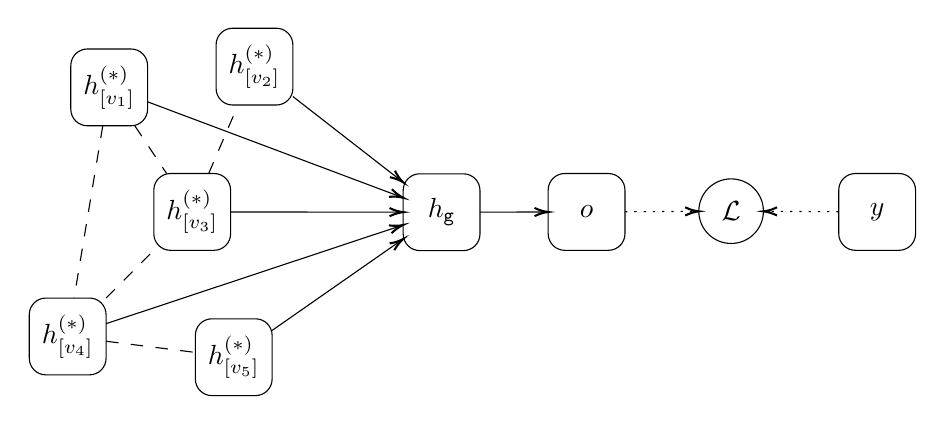
\begin{tikzpicture}[x=0.75pt,y=0.75pt,yscale=-1,xscale=1]
%uncomment if require: \path (0,300); %set diagram left start at 0, and has height of 300


% Text Node
\draw    (37.86,185.86) .. controls (37.86,181.44) and (41.44,177.86) .. (45.86,177.86) -- (66.86,177.86) .. controls (71.28,177.86) and (74.86,181.44) .. (74.86,185.86) -- (74.86,206.86) .. controls (74.86,211.28) and (71.28,214.86) .. (66.86,214.86) -- (45.86,214.86) .. controls (41.44,214.86) and (37.86,211.28) .. (37.86,206.86) -- cycle  ;
\draw (56.36,196.36) node   [align=left] {\begin{minipage}[lt]{22.249600830078126pt}\setlength\topsep{0pt}
\begin{center}
$\displaystyle \boldsymbol{h}^{( *)}_{[ v_{4}]}$
\end{center}

\end{minipage}};
% Text Node
\draw    (57.86,65.86) .. controls (57.86,61.44) and (61.44,57.86) .. (65.86,57.86) -- (86.86,57.86) .. controls (91.28,57.86) and (94.86,61.44) .. (94.86,65.86) -- (94.86,86.86) .. controls (94.86,91.28) and (91.28,94.86) .. (86.86,94.86) -- (65.86,94.86) .. controls (61.44,94.86) and (57.86,91.28) .. (57.86,86.86) -- cycle  ;
\draw (76.36,76.36) node   [align=left] {\begin{minipage}[lt]{22.249600830078126pt}\setlength\topsep{0pt}
\begin{center}
$\displaystyle \boldsymbol{h}^{( *)}_{[ v_{1}]}$
\end{center}

\end{minipage}};
% Text Node
\draw    (97.86,125.86) .. controls (97.86,121.44) and (101.44,117.86) .. (105.86,117.86) -- (126.86,117.86) .. controls (131.28,117.86) and (134.86,121.44) .. (134.86,125.86) -- (134.86,146.86) .. controls (134.86,151.28) and (131.28,154.86) .. (126.86,154.86) -- (105.86,154.86) .. controls (101.44,154.86) and (97.86,151.28) .. (97.86,146.86) -- cycle  ;
\draw (116.36,136.36) node   [align=left] {\begin{minipage}[lt]{22.249600830078126pt}\setlength\topsep{0pt}
\begin{center}
$\displaystyle \boldsymbol{h}^{( *)}_{[ v_{3}]}$
\end{center}

\end{minipage}};
% Text Node
\draw    (117.86,195.86) .. controls (117.86,191.44) and (121.44,187.86) .. (125.86,187.86) -- (146.86,187.86) .. controls (151.28,187.86) and (154.86,191.44) .. (154.86,195.86) -- (154.86,216.86) .. controls (154.86,221.28) and (151.28,224.86) .. (146.86,224.86) -- (125.86,224.86) .. controls (121.44,224.86) and (117.86,221.28) .. (117.86,216.86) -- cycle  ;
\draw (136.36,206.36) node   [align=left] {\begin{minipage}[lt]{22.249600830078126pt}\setlength\topsep{0pt}
\begin{center}
$\displaystyle \boldsymbol{h}^{( *)}_{[ v_{5}]}$
\end{center}

\end{minipage}};
% Text Node
\draw    (127.86,55.86) .. controls (127.86,51.44) and (131.44,47.86) .. (135.86,47.86) -- (156.86,47.86) .. controls (161.28,47.86) and (164.86,51.44) .. (164.86,55.86) -- (164.86,76.86) .. controls (164.86,81.28) and (161.28,84.86) .. (156.86,84.86) -- (135.86,84.86) .. controls (131.44,84.86) and (127.86,81.28) .. (127.86,76.86) -- cycle  ;
\draw (146.36,66.36) node   [align=left] {\begin{minipage}[lt]{22.249600830078126pt}\setlength\topsep{0pt}
\begin{center}
$\displaystyle \boldsymbol{h}^{( *)}_{[ v_{2}]}$
\end{center}

\end{minipage}};
% Text Node
\draw    (218,126) .. controls (218,121.58) and (221.58,118) .. (226,118) -- (247,118) .. controls (251.42,118) and (255,121.58) .. (255,126) -- (255,147) .. controls (255,151.42) and (251.42,155) .. (247,155) -- (226,155) .. controls (221.58,155) and (218,151.42) .. (218,147) -- cycle  ;
\draw (236.5,136.5) node   [align=left] {\begin{minipage}[lt]{22.249600830078126pt}\setlength\topsep{0pt}
\begin{center}
$\displaystyle \boldsymbol{h}_{\mathtt{g}}$
\end{center}

\end{minipage}};
% Text Node
\draw    (287.86,125.86) .. controls (287.86,121.44) and (291.44,117.86) .. (295.86,117.86) -- (316.86,117.86) .. controls (321.28,117.86) and (324.86,121.44) .. (324.86,125.86) -- (324.86,146.86) .. controls (324.86,151.28) and (321.28,154.86) .. (316.86,154.86) -- (295.86,154.86) .. controls (291.44,154.86) and (287.86,151.28) .. (287.86,146.86) -- cycle  ;
\draw (306.36,136.36) node   [align=left] {\begin{minipage}[lt]{22.249600830078126pt}\setlength\topsep{0pt}
\begin{center}
$\displaystyle \boldsymbol{o}$
\end{center}

\end{minipage}};
% Text Node
\draw    (376, 136) circle [x radius= 15.56, y radius= 15.56]   ;
\draw (376,136) node   [align=left] {\begin{minipage}[lt]{13.600000000000001pt}\setlength\topsep{0pt}
\begin{center}
$\displaystyle \mathcal{L}$
\end{center}

\end{minipage}};
% Text Node
\draw    (427.86,125.86) .. controls (427.86,121.44) and (431.44,117.86) .. (435.86,117.86) -- (456.86,117.86) .. controls (461.28,117.86) and (464.86,121.44) .. (464.86,125.86) -- (464.86,146.86) .. controls (464.86,151.28) and (461.28,154.86) .. (456.86,154.86) -- (435.86,154.86) .. controls (431.44,154.86) and (427.86,151.28) .. (427.86,146.86) -- cycle  ;
\draw (446.36,136.36) node   [align=left] {\begin{minipage}[lt]{22.249600830078126pt}\setlength\topsep{0pt}
\begin{center}
$\displaystyle \boldsymbol{y}$
\end{center}

\end{minipage}};
% Connection
\draw  [dash pattern={on 4.5pt off 4.5pt}]  (73.28,94.86) -- (59.44,177.86) ;
% Connection
\draw  [dash pattern={on 4.5pt off 4.5pt}]  (88.69,94.86) -- (104.03,117.86) ;
% Connection
\draw  [dash pattern={on 4.5pt off 4.5pt}]  (124.29,117.86) -- (138.43,84.86) ;
% Connection
\draw  [dash pattern={on 4.5pt off 4.5pt}]  (74.86,177.86) -- (97.86,154.86) ;
% Connection
\draw  [dash pattern={on 4.5pt off 4.5pt}]  (74.86,198.67) -- (117.86,204.05) ;
% Connection
\draw    (164.86,80.76) -- (216.42,120.88) ;
\draw [shift={(218,122.1)}, rotate = 217.89] [color={rgb, 255:red, 0; green, 0; blue, 0 }  ][line width=0.75]    (6.56,-1.97) .. controls (4.17,-0.84) and (1.99,-0.18) .. (0,0) .. controls (1.99,0.18) and (4.17,0.84) .. (6.56,1.97)   ;
% Connection
\draw    (134.86,136.38) -- (216,136.48) ;
\draw [shift={(218,136.48)}, rotate = 180.07] [color={rgb, 255:red, 0; green, 0; blue, 0 }  ][line width=0.75]    (6.56,-1.97) .. controls (4.17,-0.84) and (1.99,-0.18) .. (0,0) .. controls (1.99,0.18) and (4.17,0.84) .. (6.56,1.97)   ;
% Connection
\draw    (154.86,193.45) -- (216.36,150.55) ;
\draw [shift={(218,149.41)}, rotate = 505.1] [color={rgb, 255:red, 0; green, 0; blue, 0 }  ][line width=0.75]    (6.56,-1.97) .. controls (4.17,-0.84) and (1.99,-0.18) .. (0,0) .. controls (1.99,0.18) and (4.17,0.84) .. (6.56,1.97)   ;
% Connection
\draw    (74.86,190.21) -- (216.1,143.28) ;
\draw [shift={(218,142.65)}, rotate = 521.62] [color={rgb, 255:red, 0; green, 0; blue, 0 }  ][line width=0.75]    (6.56,-1.97) .. controls (4.17,-0.84) and (1.99,-0.18) .. (0,0) .. controls (1.99,0.18) and (4.17,0.84) .. (6.56,1.97)   ;
% Connection
\draw    (94.86,83.31) -- (216.13,128.85) ;
\draw [shift={(218,129.55)}, rotate = 200.57999999999998] [color={rgb, 255:red, 0; green, 0; blue, 0 }  ][line width=0.75]    (6.56,-1.97) .. controls (4.17,-0.84) and (1.99,-0.18) .. (0,0) .. controls (1.99,0.18) and (4.17,0.84) .. (6.56,1.97)   ;
% Connection
\draw    (255,136.46) -- (285.86,136.4) ;
\draw [shift={(287.86,136.4)}, rotate = 539.89] [color={rgb, 255:red, 0; green, 0; blue, 0 }  ][line width=0.75]    (6.56,-1.97) .. controls (4.17,-0.84) and (1.99,-0.18) .. (0,0) .. controls (1.99,0.18) and (4.17,0.84) .. (6.56,1.97)   ;
% Connection
\draw  [dash pattern={on 0.84pt off 2.51pt}]  (324.86,136.26) -- (358.44,136.09) ;
\draw [shift={(360.44,136.08)}, rotate = 539.7] [color={rgb, 255:red, 0; green, 0; blue, 0 }  ][line width=0.75]    (6.56,-1.97) .. controls (4.17,-0.84) and (1.99,-0.18) .. (0,0) .. controls (1.99,0.18) and (4.17,0.84) .. (6.56,1.97)   ;
% Connection
\draw  [dash pattern={on 0.84pt off 2.51pt}]  (427.86,136.27) -- (393.56,136.09) ;
\draw [shift={(391.56,136.08)}, rotate = 360.28999999999996] [color={rgb, 255:red, 0; green, 0; blue, 0 }  ][line width=0.75]    (6.56,-1.97) .. controls (4.17,-0.84) and (1.99,-0.18) .. (0,0) .. controls (1.99,0.18) and (4.17,0.84) .. (6.56,1.97)   ;

\end{tikzpicture}}
    \caption{A graph readout on an example graph for a graph classification/regression task. Here, we assume the node representations $\StateVector{v}{*}$ have already been obtained by a node readout (not shown).}
    \label{fig:graph-readout}
\end{figure*}
A graph readout applied to an example graph is shown in Figure \ref{fig:graph-readout}.

\subsubsection*{Graph Pooling Layers}\label{sec:pooling}
Similarly to the layer used by \glspl{cnn} for computer vision, pooling is also applicable to \glspl{dgn} for graph classification (or regression) tasks. In \gls{dgn} architectures, pooling is usually placed after a graph convolutional layer, and serves a three-fold purpose: it is used to detect communities in the graph, \ie clusters of nodes with higher connectivity among themselves than the rest of the graph; to augment the information content of the hidden states with this knowledge; and to reduce the number of nodes (and consequently, the number of parameters) needed by the network in later stages of computation. An example of a graph pooling layer is shown in Figure \ref{fig:pooling}, where nearby nodes are pooled into a single node in the reduced graph according to some strategy. Graph pooling methods are developed according to two strategies: \emph{adaptive} and \emph{tolopogical}. Adaptive methods pool nodes in a differentiable manner, so that the optimal clustering of the nodes for the task at hand is learned by the end-to-end network. One example of adaptive pooling is DiffPool, developed by \citet{ying2018diffpool}. Given an attributed graph $\Graph{G}$ with $n$ nodes, and assuming the $\ell-1$ \glspl{gcl} have been applied, DiffPool computes two matrices:
\begin{align*}
    \GenGraphLayerMat{z}{\ell-1} &= \Fun{S}_e(\LayerAdjMat{\ell-1},\LayerStateMat{\ell-1}) \in \Real^{n \times h}\\
    \GenGraphLayerMat{s}{\ell-1} &= \softmax\Par{\Fun{S}_p(\LayerAdjMat{\ell-1},\LayerStateMat{\ell-1})} \in \Real^{n \times k},
\end{align*}
where $\Fun{S}_e$ and $\Fun{S}_p$ are stacks of graph convolutional layers. The matrix $\Matrix{S}$ learns a soft-assignment to each node to one of $k$ clusters with a softmax output function. These two matrices are then combined with the current hidden states to produce a novel adjacency matrix and its corresponding matrix of hidden states as follows:
\begin{align*}
    \LayerStateMat{\ell} &= \GenGraphLayerMat{s}{\ell-1}\GenGraphLayerMat{z}{\ell-1} \in \Real^{k \times h}\\
    \LayerAdjMat{\ell} &= \GenGraphLayerMat{s}{\ell-1}\LayerAdjMat{\ell-1}\GenGraphLayerMat{s}{\ell-1} \in \Real^{k \times k}
\end{align*}
where $\LayerAdjMat{0} = \AdjMatrix{g}$ and $\LayerStateMat{0} = \FeatureMatrix{g}$. Thus, after applying the DiffPool layer, the size of the graph is reduced progressively from $n$ to $k$ nodes.

\begin{figure*}[h!]
    \centering
    \resizebox{.8\textwidth}{!}{

\tikzset{every picture/.style={line width=0.75pt}} %set default line width to 0.75pt        

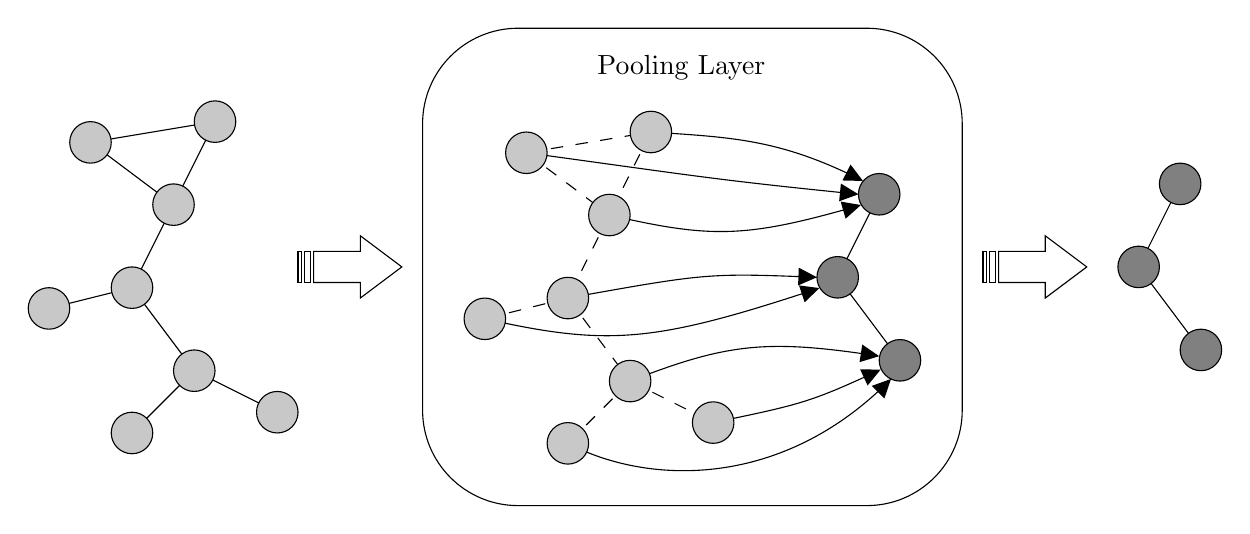
\begin{tikzpicture}[x=0.75pt,y=0.75pt,yscale=-1,xscale=1]
%uncomment if require: \path (0,300); %set diagram left start at 0, and has height of 300

%Straight Lines [id:da5096617344365821] 
\draw    (585,95) -- (565,135) ;
%Straight Lines [id:da9932827718765578] 
\draw    (565,135) -- (595,175) ;
%Curve Lines [id:da6905034262446312] 
\draw    (270,80) .. controls (352.62,91.31) and (359.81,92.89) .. (427.92,99.79) ;
\draw [shift={(430,100)}, rotate = 185.77] [fill={rgb, 255:red, 0; green, 0; blue, 0 }  ][line width=0.08]  [draw opacity=0] (8.93,-4.29) -- (0,0) -- (8.93,4.29) -- cycle    ;
%Curve Lines [id:da8335321724765272] 
\draw    (330,70) .. controls (368.17,72.52) and (391.5,73.29) .. (429.83,92.38) ;
\draw [shift={(432.2,93.58)}, rotate = 207] [fill={rgb, 255:red, 0; green, 0; blue, 0 }  ][line width=0.08]  [draw opacity=0] (8.93,-4.29) -- (0,0) -- (8.93,4.29) -- cycle    ;
%Curve Lines [id:da31100259312110135] 
\draw    (250,160) .. controls (309.35,173.29) and (331.51,171.46) .. (408.84,145.96) ;
\draw [shift={(411.2,145.18)}, rotate = 521.6700000000001] [fill={rgb, 255:red, 0; green, 0; blue, 0 }  ][line width=0.08]  [draw opacity=0] (8.93,-4.29) -- (0,0) -- (8.93,4.29) -- cycle    ;
%Curve Lines [id:da5677680537011585] 
\draw    (320,190) .. controls (366.25,171.95) and (385.37,169.74) .. (437.59,177.63) ;
\draw [shift={(440,178)}, rotate = 188.76] [fill={rgb, 255:red, 0; green, 0; blue, 0 }  ][line width=0.08]  [draw opacity=0] (8.93,-4.29) -- (0,0) -- (8.93,4.29) -- cycle    ;
%Curve Lines [id:da15435588971241] 
\draw    (360,210) .. controls (401.63,201.4) and (406.71,200.23) .. (438.22,185.63) ;
\draw [shift={(440.7,184.48)}, rotate = 515.05] [fill={rgb, 255:red, 0; green, 0; blue, 0 }  ][line width=0.08]  [draw opacity=0] (8.93,-4.29) -- (0,0) -- (8.93,4.29) -- cycle    ;
%Curve Lines [id:da7751491360366476] 
\draw    (290,220) .. controls (327.57,239.78) and (391.65,242.62) .. (444.11,190.57) ;
\draw [shift={(445.7,188.98)}, rotate = 494.49] [fill={rgb, 255:red, 0; green, 0; blue, 0 }  ][line width=0.08]  [draw opacity=0] (8.93,-4.29) -- (0,0) -- (8.93,4.29) -- cycle    ;
%Curve Lines [id:da9997311294079065] 
\draw    (310,110) .. controls (358.71,121.25) and (375.45,121.18) .. (428.74,105.88) ;
\draw [shift={(431.2,105.17)}, rotate = 523.85] [fill={rgb, 255:red, 0; green, 0; blue, 0 }  ][line width=0.08]  [draw opacity=0] (8.93,-4.29) -- (0,0) -- (8.93,4.29) -- cycle    ;
%Curve Lines [id:da5516088460235944] 
\draw    (290,150) .. controls (356.19,138.11) and (357.67,137.93) .. (407.68,139.91) ;
\draw [shift={(410,140)}, rotate = 182.27] [fill={rgb, 255:red, 0; green, 0; blue, 0 }  ][line width=0.08]  [draw opacity=0] (8.93,-4.29) -- (0,0) -- (8.93,4.29) -- cycle    ;
%Straight Lines [id:da42002527970780945] 
\draw    (60,75) -- (100,105) ;
%Straight Lines [id:da9625123729833738] 
\draw    (120,65) -- (100,105) ;
%Straight Lines [id:da011564512705323882] 
\draw    (60,75) -- (120,65) ;
%Straight Lines [id:da591791700605113] 
\draw    (100,105) -- (80,145) ;
%Straight Lines [id:da0520483680630226] 
\draw    (40,155) -- (80,145) ;
%Straight Lines [id:da243342242168614] 
\draw    (80,145) -- (110,185) ;
%Straight Lines [id:da29763945544745907] 
\draw    (110,185) -- (80,215) ;
%Straight Lines [id:da041191991130072436] 
\draw    (110,185) -- (150,205) ;
%Shape: Circle [id:dp7340107223648733] 
\draw  [fill={rgb, 255:red, 200; green, 200; blue, 200 }  ,fill opacity=1 ] (50,75) .. controls (50,69.48) and (54.48,65) .. (60,65) .. controls (65.52,65) and (70,69.48) .. (70,75) .. controls (70,80.52) and (65.52,85) .. (60,85) .. controls (54.48,85) and (50,80.52) .. (50,75) -- cycle ;
%Shape: Circle [id:dp00026389043378993726] 
\draw  [fill={rgb, 255:red, 200; green, 200; blue, 200 }  ,fill opacity=1 ] (110,65) .. controls (110,59.48) and (114.48,55) .. (120,55) .. controls (125.52,55) and (130,59.48) .. (130,65) .. controls (130,70.52) and (125.52,75) .. (120,75) .. controls (114.48,75) and (110,70.52) .. (110,65) -- cycle ;
%Shape: Circle [id:dp5553734560288552] 
\draw  [fill={rgb, 255:red, 200; green, 200; blue, 200 }  ,fill opacity=1 ] (90,105) .. controls (90,99.48) and (94.48,95) .. (100,95) .. controls (105.52,95) and (110,99.48) .. (110,105) .. controls (110,110.52) and (105.52,115) .. (100,115) .. controls (94.48,115) and (90,110.52) .. (90,105) -- cycle ;
%Shape: Circle [id:dp7685657012179221] 
\draw  [fill={rgb, 255:red, 200; green, 200; blue, 200 }  ,fill opacity=1 ] (70,145) .. controls (70,139.48) and (74.48,135) .. (80,135) .. controls (85.52,135) and (90,139.48) .. (90,145) .. controls (90,150.52) and (85.52,155) .. (80,155) .. controls (74.48,155) and (70,150.52) .. (70,145) -- cycle ;
%Shape: Circle [id:dp8225576337985958] 
\draw  [fill={rgb, 255:red, 200; green, 200; blue, 200 }  ,fill opacity=1 ] (30,155) .. controls (30,149.48) and (34.48,145) .. (40,145) .. controls (45.52,145) and (50,149.48) .. (50,155) .. controls (50,160.52) and (45.52,165) .. (40,165) .. controls (34.48,165) and (30,160.52) .. (30,155) -- cycle ;
%Shape: Circle [id:dp8048870433512154] 
\draw  [fill={rgb, 255:red, 200; green, 200; blue, 200 }  ,fill opacity=1 ] (100,185) .. controls (100,179.48) and (104.48,175) .. (110,175) .. controls (115.52,175) and (120,179.48) .. (120,185) .. controls (120,190.52) and (115.52,195) .. (110,195) .. controls (104.48,195) and (100,190.52) .. (100,185) -- cycle ;
%Shape: Circle [id:dp3899524469262352] 
\draw  [fill={rgb, 255:red, 200; green, 200; blue, 200 }  ,fill opacity=1 ] (70,215) .. controls (70,209.48) and (74.48,205) .. (80,205) .. controls (85.52,205) and (90,209.48) .. (90,215) .. controls (90,220.52) and (85.52,225) .. (80,225) .. controls (74.48,225) and (70,220.52) .. (70,215) -- cycle ;
%Shape: Circle [id:dp40591726527712235] 
\draw  [fill={rgb, 255:red, 200; green, 200; blue, 200 }  ,fill opacity=1 ] (140,205) .. controls (140,199.48) and (144.48,195) .. (150,195) .. controls (155.52,195) and (160,199.48) .. (160,205) .. controls (160,210.52) and (155.52,215) .. (150,215) .. controls (144.48,215) and (140,210.52) .. (140,205) -- cycle ;
%Straight Lines [id:da673763044302859] 
\draw  [dash pattern={on 4.5pt off 4.5pt}]  (270,80) -- (310,110) ;
%Straight Lines [id:da9124441607803917] 
\draw  [dash pattern={on 4.5pt off 4.5pt}]  (330,70) -- (310,110) ;
%Straight Lines [id:da03995998781592447] 
\draw  [dash pattern={on 4.5pt off 4.5pt}]  (270,80) -- (330,70) ;
%Straight Lines [id:da8129344208516425] 
\draw  [dash pattern={on 4.5pt off 4.5pt}]  (310,110) -- (290,150) ;
%Straight Lines [id:da6336124502461815] 
\draw  [dash pattern={on 4.5pt off 4.5pt}]  (250,160) -- (290,150) ;
%Straight Lines [id:da8022108969555355] 
\draw  [dash pattern={on 4.5pt off 4.5pt}]  (290,150) -- (320,190) ;
%Straight Lines [id:da3098627478952969] 
\draw  [dash pattern={on 4.5pt off 4.5pt}]  (320,190) -- (290,220) ;
%Straight Lines [id:da14837892723690072] 
\draw  [dash pattern={on 4.5pt off 4.5pt}]  (320,190) -- (360,210) ;
%Shape: Circle [id:dp42990613199323735] 
\draw  [fill={rgb, 255:red, 200; green, 200; blue, 200 }  ,fill opacity=1 ] (260,80) .. controls (260,74.48) and (264.48,70) .. (270,70) .. controls (275.52,70) and (280,74.48) .. (280,80) .. controls (280,85.52) and (275.52,90) .. (270,90) .. controls (264.48,90) and (260,85.52) .. (260,80) -- cycle ;
%Shape: Circle [id:dp2754617992158239] 
\draw  [fill={rgb, 255:red, 200; green, 200; blue, 200 }  ,fill opacity=1 ] (320,70) .. controls (320,64.48) and (324.48,60) .. (330,60) .. controls (335.52,60) and (340,64.48) .. (340,70) .. controls (340,75.52) and (335.52,80) .. (330,80) .. controls (324.48,80) and (320,75.52) .. (320,70) -- cycle ;
%Shape: Circle [id:dp21321858378283642] 
\draw  [fill={rgb, 255:red, 200; green, 200; blue, 200 }  ,fill opacity=1 ] (300,110) .. controls (300,104.48) and (304.48,100) .. (310,100) .. controls (315.52,100) and (320,104.48) .. (320,110) .. controls (320,115.52) and (315.52,120) .. (310,120) .. controls (304.48,120) and (300,115.52) .. (300,110) -- cycle ;
%Shape: Circle [id:dp5661953542799116] 
\draw  [fill={rgb, 255:red, 200; green, 200; blue, 200 }  ,fill opacity=1 ] (280,150) .. controls (280,144.48) and (284.48,140) .. (290,140) .. controls (295.52,140) and (300,144.48) .. (300,150) .. controls (300,155.52) and (295.52,160) .. (290,160) .. controls (284.48,160) and (280,155.52) .. (280,150) -- cycle ;
%Shape: Circle [id:dp5442339392428344] 
\draw  [fill={rgb, 255:red, 200; green, 200; blue, 200 }  ,fill opacity=1 ] (240,160) .. controls (240,154.48) and (244.48,150) .. (250,150) .. controls (255.52,150) and (260,154.48) .. (260,160) .. controls (260,165.52) and (255.52,170) .. (250,170) .. controls (244.48,170) and (240,165.52) .. (240,160) -- cycle ;
%Shape: Circle [id:dp00011290407505515354] 
\draw  [fill={rgb, 255:red, 200; green, 200; blue, 200 }  ,fill opacity=1 ] (310,190) .. controls (310,184.48) and (314.48,180) .. (320,180) .. controls (325.52,180) and (330,184.48) .. (330,190) .. controls (330,195.52) and (325.52,200) .. (320,200) .. controls (314.48,200) and (310,195.52) .. (310,190) -- cycle ;
%Shape: Circle [id:dp518700726149034] 
\draw  [fill={rgb, 255:red, 200; green, 200; blue, 200 }  ,fill opacity=1 ] (280,220) .. controls (280,214.48) and (284.48,210) .. (290,210) .. controls (295.52,210) and (300,214.48) .. (300,220) .. controls (300,225.52) and (295.52,230) .. (290,230) .. controls (284.48,230) and (280,225.52) .. (280,220) -- cycle ;
%Shape: Circle [id:dp5730004415356564] 
\draw  [fill={rgb, 255:red, 200; green, 200; blue, 200 }  ,fill opacity=1 ] (350,210) .. controls (350,204.48) and (354.48,200) .. (360,200) .. controls (365.52,200) and (370,204.48) .. (370,210) .. controls (370,215.52) and (365.52,220) .. (360,220) .. controls (354.48,220) and (350,215.52) .. (350,210) -- cycle ;
%Straight Lines [id:da001623419930635972] 
\draw    (440,100) -- (420,140) ;
%Straight Lines [id:da015699553757238416] 
\draw    (420,140) -- (450,180) ;
%Shape: Circle [id:dp36211696768410073] 
\draw  [fill={rgb, 255:red, 128; green, 128; blue, 128 }  ,fill opacity=1 ] (430,100) .. controls (430,94.48) and (434.48,90) .. (440,90) .. controls (445.52,90) and (450,94.48) .. (450,100) .. controls (450,105.52) and (445.52,110) .. (440,110) .. controls (434.48,110) and (430,105.52) .. (430,100) -- cycle ;
%Shape: Circle [id:dp01799126024681974] 
\draw  [fill={rgb, 255:red, 128; green, 128; blue, 128 }  ,fill opacity=1 ] (410,140) .. controls (410,134.48) and (414.48,130) .. (420,130) .. controls (425.52,130) and (430,134.48) .. (430,140) .. controls (430,145.52) and (425.52,150) .. (420,150) .. controls (414.48,150) and (410,145.52) .. (410,140) -- cycle ;
%Shape: Circle [id:dp058899920078356205] 
\draw  [fill={rgb, 255:red, 128; green, 128; blue, 128 }  ,fill opacity=1 ] (440,180) .. controls (440,174.48) and (444.48,170) .. (450,170) .. controls (455.52,170) and (460,174.48) .. (460,180) .. controls (460,185.52) and (455.52,190) .. (450,190) .. controls (444.48,190) and (440,185.52) .. (440,180) -- cycle ;
%Shape: Circle [id:dp5649766452502909] 
\draw  [fill={rgb, 255:red, 128; green, 128; blue, 128 }  ,fill opacity=1 ] (575,95) .. controls (575,89.48) and (579.48,85) .. (585,85) .. controls (590.52,85) and (595,89.48) .. (595,95) .. controls (595,100.52) and (590.52,105) .. (585,105) .. controls (579.48,105) and (575,100.52) .. (575,95) -- cycle ;
%Shape: Circle [id:dp5246365191278834] 
\draw  [fill={rgb, 255:red, 128; green, 128; blue, 128 }  ,fill opacity=1 ] (555,135) .. controls (555,129.48) and (559.48,125) .. (565,125) .. controls (570.52,125) and (575,129.48) .. (575,135) .. controls (575,140.52) and (570.52,145) .. (565,145) .. controls (559.48,145) and (555,140.52) .. (555,135) -- cycle ;
%Shape: Circle [id:dp5766159917435185] 
\draw  [fill={rgb, 255:red, 128; green, 128; blue, 128 }  ,fill opacity=1 ] (585,175) .. controls (585,169.48) and (589.48,165) .. (595,165) .. controls (600.52,165) and (605,169.48) .. (605,175) .. controls (605,180.52) and (600.52,185) .. (595,185) .. controls (589.48,185) and (585,180.52) .. (585,175) -- cycle ;
%Rounded Rect [id:dp6303563718720424] 
\draw   (220,66) .. controls (220,40.59) and (240.59,20) .. (266,20) -- (434,20) .. controls (459.41,20) and (480,40.59) .. (480,66) -- (480,204) .. controls (480,229.41) and (459.41,250) .. (434,250) -- (266,250) .. controls (240.59,250) and (220,229.41) .. (220,204) -- cycle ;
%Striped Right Arrow [id:dp8981402107639092] 
\draw   (167.5,127.5) -- (190,127.5) -- (190,120) -- (210,135) -- (190,150) -- (190,142.5) -- (167.5,142.5) -- cycle ;\draw   (160,127.5) -- (161.5,127.5) -- (161.5,142.5) -- (160,142.5) -- cycle ;\draw   (163,127.5) -- (166,127.5) -- (166,142.5) -- (163,142.5) -- cycle ;
%Striped Right Arrow [id:dp4519194983259933] 
\draw   (497.5,127.5) -- (520,127.5) -- (520,120) -- (540,135) -- (520,150) -- (520,142.5) -- (497.5,142.5) -- cycle ;\draw   (490,127.5) -- (491.5,127.5) -- (491.5,142.5) -- (490,142.5) -- cycle ;\draw   (493,127.5) -- (496,127.5) -- (496,142.5) -- (493,142.5) -- cycle ;

% Text Node
\draw (303,32) node [anchor=north west][inner sep=0.75pt]   [align=left] {Pooling Layer};


\end{tikzpicture}}
    \caption{A visual example of a graph pooling layer.}
    \label{fig:pooling}
\end{figure*}
Topological pooling, on the other hand,  uses not-differentiable methods which leverage the global structure of the graph, and the communities beneath it. These methods work by grouping nodes according to well known graph theory tools, such as spectral clustering (see \eg \citet{vonluxburg2007tutorialspectralclustering, dhillon2007weightedgraphcuts}).

\subsection{Regularization}
\glspl{dgn} are trained with regular losses, such as \gls{ce} for classification and \gls{mse} for regression. Besides standard regularization techniques, the objective function is often regularized through unsupervised loss functions, which impose priors on which kind of structures the network should preferably learn. The regularized objective function for supervised tasks\footnote{We use a generic target $y$ to imply that this formulation is task-independent.} has the form:
$$\argmin_{\Param} \Loss(\Param, (\Vector{x}_{\Graph{g}}, y)) + \lambda \sum_{\ell=1}^L \Psi(\LayerStateMat{\ell}),$$
were $\Psi$ is a regularization function weighted by a regularization coefficient $\lambda$, that is applied at each layer $\ell$ to the set of hidden states of the nodes, represented as a matrix $\Matrix{h}_{{\Graph{g}}}^{(\ell)} \in \Real^{n \times h}$. An example of regularization widely employed in practical settings is the \emph{link prediction} unsupervised loss, defined as:
\begin{align}
    \Psi(\LayerStateMat{\ell}) = \sum_{u,v} \Norm{\StateVector{v}{\ell} - \StateVector{u}{\ell}}_2,
\end{align}
where the summation ranges over all possible combinations of nodes. Basically, when this loss is minimized, it biases the network towards producing node representations that are more similar for nodes connected by an edge. Notably, this loss can be also used in isolation to tackle link prediction tasks, \ie tasks where the downstream network must predict unseen links between the nodes.

\section{Deep Generative Learning of Graphs}
In this section, we discuss the graph generation problem. The term \quotes{graph generation} is purposely kept broad, to include a variety of methodologies which learn processes that generate graphs from a set of training examples. This research field originates from generative models of graphs for the theoretical understanding of graph properties, which have been studied thoroughly since the '50s in the field of graph theory. The first known generative model is the  Erd\"{o}s-R\'{e}nyi (ER) model \cite{erdos1959randomgraphs}. The ER model studies random graphs, where the connectivity among graph nodes is modeled independently. This model is useful to study theoretical properties of graphs, such as how the global connectivity of the graph evolves as its size grows. Another historical model of graphs is the  Watts-Strogatz (WS)  model \cite{watts1998smallworld}. The WS model concerns \quotes{small world} graphs, \ie graphs where it is possible to reach any other node in the graph with very short paths, regardless of their size. This property arises in several real-world graphs such as social and electrical networks. Lastly, the Barab{\'a}si-Albert (BA) model \cite{barabasi1999prefatt}, which models the so-called \quotes{preferential attachment} property, where the connectivity potential of a node is directly proportional to its number of neighbors. While being useful to the study and understanding of graph properties, these models usually fail to generalize to real-world graph distributions, because they can only model one or a limited number of graph properties; moreover, their parameters cannot be learned from data in general. Other methods such as stochastic block models \citep{airoldi2008mixedstochasticblock}, exponential random graphs \citep{robins2007exponentialrandomgraphs}, and Kronecker graphs \citep{leskovec2010kronecker} can approximate more complex graph distributions such as graphs with communities, but are still limited to specific kinds of graphs and scale poorly to large datasets.
These limitations clearly highlight that, in order to generate graphs for practical applications, a more powerful class of learning models is needed. In this section, we review a variety of generative models of graphs based on Deep Learning approaches. The advantages of such models are the possibility to approximate complex distributions efficiently and effectively, and the flexibility to use different generative paradigms to adapt to the task at hand.

\subsection{The Challenges of Graph Generation}
The problem of generating graph structures from arbitrary distributions is arguably harder than predictive modeling. Some of the challenges that need to be addressed when designing deep generative models of graphs are related to the complexity of graph spaces. In particular, we report the following:
\begin{itemize}
    \item \emph{size of graphs spaces}. Graphs spaces are combinatorial, and thus very large. For example, the size of the space of undirected graphs with $m$ nodes is ${m \choose 2} = \frac{m(m-1)}{2}$, which becomes very large even for graphs with a moderate number of nodes. Thus, trivial approaches such as exhaustive enumeration are generally intractable. Moreover, real-world graph distributions are usually defined over attributed graphs with variable size, which makes the search space even larger;
    \item \emph{discreteness of graphs spaces}. Graphs are discrete objects. This contrasts with the nature of neural networks, which can back-propagate only through continuous and differentiable objects. Hence, the learning process must be adjusted to work with discrete structures;
    \item \emph{sparsity of graphs spaces}. For most generative tasks, only very small subsets of graph space contain graphs with non-zero probability. Thus, any generative method should be designed to focus on regions where interesting graphs are contained, to avoid efficiency issues;
    \item \emph{complex dependencies}. Most real-world graph have hard structural constraints that are very difficult to enforce on a generative model (which is inherently stochastic). For example, cycle graphs are such that if only one edge is misplaced, the graph is not a cycle anymore;
    \item \emph{non-unique representations}. In general, graphs are invariant under node permutation. Thus, the same graph can be potentially represented by up to $n!$ possible adjacency matrices, depending on the node permutation. This poses constraints on the kind of graph representations a generative model can learn. For example, generative methods that map graphs into a latent space must take into account that different node permutations of the same graph must map to the same latent vector. While invariance to node permutation can be addressed by assuming an order of the graph nodes, this introduces the problem of maintaining order consistency among different graphs.
\end{itemize}

\subsection{Generative Tasks}
The family of \glspl{dgm} of graphs is flexible enough to model different kinds of generative tasks. Assuming unattributed graphs for simplicity, we loosely follow the taxonomy proposed by \citet{guo2020systematicreviewgenerativegraphs} and distinguish two main tasks related to graph generation:
\begin{itemize}
    \item \emph{unconditional generation}, where the task is to explicitly learn a distribution $p(\Graph{g})$ over graphs, or some parameterized function that produces samples from it. Here, the term \quotes{unconditional} refers to the fact that the generation starts with drawing a vector $\Vector{z} \in \Real^z$ from some easy to sample prior distribution $p(\Vector{z})$, which is usually assumed to be an isotropic Gaussian or a uniform distribution;
    \item \emph{conditional generation}, where the aim is to learn a conditional distribution $p(\Graph{g} \given \Vector{y})$ with $\Vector{y} \in \Real^y$, or the corresponding parameterized sampling mechanism. The purpose of the conditioning vector is to drive the generative process towards producing a graph with desired characteristics. For example, one might want to generate a graph whose structure resembles that of a graph given as input to the \gls{dgm}. In this case, $\Vector{y}$ is the representation of the conditioning graph.
\end{itemize}
Hereafter, we consider the task of unconditional generation, where we assume access to a dataset of graphs $\Data = \Set{\Graph{g}_i}_{i=1}^n$. Broadly speaking, defining a \gls{dgm} of graphs requires specifying two components: a \emph{graph decoder}, which takes care of generating a graph, and an end-to-end generative framework used to optimize the model parameters. As regards the latter, common generative frameworks include \glspl{vae}, \glspl{gan}, and flow-based models \citep{rezende2015normalizingflows}. Here, we only describe approaches based on the first two.

\subsection{Graph Decoders}
The graph decoder is the architectural component that outputs some conditional distribution, which can be sampled to generate a graph. If the framework in which the decoder is placed allows for inference (such as the \gls{vae}), the conditional can be learned with \gls{mle}; otherwise, (such as with \glspl{gan}) it is used only for sampling, and its parameters are optimized with adversarial training. Ideally, graph decoders should generate permutation invariant graphs; however, this is rarely the case. The major hurdle to devise permutation invariant graph decoders is their computational cost; even though some methods do exist \citep{ermon2020permutationinvariantgraphgeneration}, they are still too inefficient to be deployed in real world scenarios. Thus, in the following, we assume non-invariance.
One particular caveat that needs to be addressed during the training phase of a graph decoder is maintaining the differentiability of the architecture while still generating hard graph samples. This is critical especially in \gls{gan}-like architectures, where the discriminator must be trained with actual graphs. As with sequence generation with \glspl{rnn}, the same techniques (straight-through gradient estimation \cite{bengio2013straighttrough}, reparameterization \cite{kingma2014vae}, or even reinforcement learning-based techniques \cite{williams1992reinforce}) can be used for this purpose. There are two main paradigms to implement adaptive graph decoders, which we detail in the following.

\subsubsection*{One-shot Decoders}
This class of graph decoders outputs a dense probabilistic adjacency matrix $\ProbAdjMatrix{g} \in \Real^{n \times n}$, where $n$ is the maximum number of nodes allowed. The probabilistic matrix is sampled entry by entry to produce an actual adjacency matrix. The entries of the matrix are modeled as independent Bernoulli variables, which indicate the presence or absence of an edge. Generally, the elements in the adjacency matrix $a_{ii}$ are modeled as independent Bernoulli variables that specify if a node belongs to the graph or not. In practice, the entries of the matrix are produced by a neural network with sigmoid outputs that predicts an $n \times n$ vector. Thus, the adjacency matrix can be sampled in parallel (hence the term \quotes{one-shot}). Two possible approaches to specify a one-shot decoder are:

\begin{itemize}
    \item \emph{graph-based} decoders, which require a graph representation $\Vector{z}$. In this case, the decoder models the conditional as follows:
    $$p(\ProbAdjMatrix{g} \given \Vector{z}) \approx p(\ProbAdjMatrix{g} \given \Vector{z}) = p_{\Param}(\Vector{z}),$$
    where $p_{\Param}$ is a neural network with sigmoid outputs that predicts the matrix from the graph representation;
    \item \emph{node-based} decoders, which require a matrix of node representations $\Matrix{Z} \in \Real^{n \times z}$. In this case, the decoder models the conditional as follows:
    $$p(\ProbAdjMatrix{g} \given \Matrix{z}) \approx \prod_{i=1}^n \prod_{j=1}^n p(a_{ij} \given \Vector{z}_i, \Vector{z}_j) = \prod_{i=1}^n \prod_{j=1}^n p_{\Param}(\Vector{z}_i\Vector{z}_j),$$
    where $i$ and $j$ range over the matrix rows, and $p_{\Param}$ is a neural network that takes as input a pair of node representations, and applies a sigmoid function to their dot product. The idea is that nodes that are close in representation space should be more likely to be connected.
\end{itemize}
One-shot approaches are usually fast to train and to take samples from. However, they are too simplistic, in that they assume the edges are generated independently (which is usually not the case for real-world graphs). Furthermore, the maximum number of nodes must be pre-specified, which makes them unable to generalize to larger graphs.

\subsubsection*{Autoregressive Decoders}
Autoregressive decoders assume that graphs are generated by some sequential process that involves its set of nodes. Specifically, the generative process is the following:
$$p(\Graph{s}) = \int p(\Graph{s}, \pi)\, d\pi = \int p(\Graph{s} \given \pi)\, q(\pi)\, d\pi,$$
where $\Graph{s}$ are sequences that generate graphs one component at a time, and the order of generation is given directly or indirectly by a node permutation drawn from a prior $q(\pi)$. The idea is to decompose the generating sequence autoregressively as follows:
$$p(\Graph{s}) = \int p(\Graph{s}_i \given \Graph{s}_{<i}, \pi)\, q(\pi)\, d\pi.$$
However, this requires to integrate over all $n!$ possible node permutations, which becomes intractable for moderately large graphs. An approximate solution to this issue is to assume some ordering and create the sequences before training, as a preprocessing step. Once the sequence are fixed, the chain-rule decomposition becomes tractable:
$$p(\Graph{s}) \approx p_{\Param}^{\pi}(\Graph{s}) = p_{\Param}^{\pi}(\Graph{s}_i \given \Graph{s}_{<i}).$$
Depending on the nature of the graph generating sequence, we distinguish four possible approaches to develop autoregressive graph decoders:
\begin{itemize}
    \item \emph{node-based} approaches decompose the graph as a sequence of actions performed on an initially empty graph. These action correspond to decisions such as whether to add a node to the existing graph, and which nodes it must be connected to. In this case, $\Graph{s}_{<i}$ is a vector that represents the current state of the graph. For all these models, one has two options as to how to implement the autoregressive network. One approach is to use a hierarchy of \glspl{rnn}: one keeps track of the state of the nodes added to the graph, and the other is responsible to connect newly added nodes to the current graph, given the state of the first \citep{you2018graphrnn}. The other choice is to update the state of the current graph with a \gls{dgn}. This state is passed to the networks responsible for deciding which action to perform \citep{li2018learningdeepgmg};
    \item \emph{edge-based} approaches decompose the graph as a sequence of edges. To produce an ordered sequence of edges, one must first order its nodes, then label the nodes with progressive integers, and then sort its set of edges in lexicographic order. In this case, $\Graph{s}_{<i}$ represents the state of the graph indirectly, by keeping memory of the edges of the sequence already generated. These approaches are mostly implemented with \glspl{rnn} \citep{goyal2020graphgen,bacciu2019edgegraphgenrnn};
    \item \emph{rule-based} approaches can be applied in cases where the graph generation can be decomposed in a sequence of production rules over some known grammar (\eg for molecules or computer programs) \citep{kusner2017grammarvae,dai2018sdvae}. In this case, the model generates a sequence of production rules to construct a desired graph;
    \item \emph{motif-based} approaches decompose the graph as a sequence (or even a tree) of \emph{motifs}, \ie very small and manageable subgraphs, which are combined adaptively. Here, the challenge is mainly how to decompose the graphs into sequences of motifs.
\end{itemize}
A special kind of sequential decomposition for graphs is the \gls{smiles} linearization applied to molecules. We shall define the SMILES more precisely in Section \ref{subsec:smiles}; for the moment, it is sufficient to say that the SMILES encoding of a molecule is a string of ASCII characters that represents its structure. When a domain-specific linearization techniques such as SMILES is not available, the sequences representing the graph generative process are constructed based on some node ordering strategy. One general strategy to do so is to choose one node at random, then visit the graph nodes with a depth-first or breadth-first traversal. The order by which the nodes are visited is used to determine the order of the elements in the sequences. Clearly, this approach is not optimal since it heavily depends on the starting node, and may produce very different sequences for different starting node choices. However, it has been shown to work empirically \citep{you2018graphrnn,li2018learningdeepgmg,bacciu2019edgegraphgenrnn,goyal2020graphgen}. The pros and cons of autoregressive decoders are orthogonal to those of one-shot decoders: briefly, they allow generating variable-sized graphs seamlessly, and they can model dependencies between nodes and edges by means of the autoregressive property. However, both training and sampling processes are slower in terms of computational time, because the graphs are reconstructed one sequence element at a time and not in parallel.

\subsection{Performance Evaluation}\label{sec:evaluation-generative-graphs}
The desired end result of training a generative model is that the structure of samples generated by the network should resemble that of graphs in the training set, without being identical. This is more challenging with respect to predictive tasks, since the samples of a generative model do not exist until they are generated. Hence, there are no strong guarantees that the learned distribution is the correct one. Furthermore, the model can very easily obtain misleading performances by learning to replicate training graphs exactly, or repeating the same graph typology over and over. Thus, one critical aspect of using generative models of graphs is how to assess performances. Below, we define two broad classes of metrics that allow the evaluation of graph models, assuming the availability of a training sample $\TrainingSample \subseteq \Data = \Set{\Graph{g}}_{i=1}^n$, and a collection\footnote{Here, we use the term \quotes{collection} to indicate a multiset, meaning that it can possibly contain duplicate elements.} $\GeneratedSample = \Set{\Graph{g'}}_{i=1}^m$ of samples generated by the model.

\subsubsection*{Quantitative Metrics}
\emph{Quantitative} metrics measure the rate at which the generative model produces diverse and heterogeneous graphs, without taking into account structural similarity. The three main quantitative metrics considered in the literature are:
\begin{itemize}
    \item \emph{novelty} measures the ratio of generated samples that are not training samples. A high novelty indicates that the model has not learned to replicate training graphs. Conversely, low novelty indicates that the model has overfit the training data. Formally, it is measured as $1 - \frac{|\GeneratedSample \Inter \TrainingSample|}{|\TrainingSample|}$;
    \item \emph{uniqueness} measures the ratio of unique graphs with respect to the total number of graphs generated. A low uniqueness rate might indicate that the model has overfit one specific graph structure. To calculate uniqueness, one first checks every graph for isomorphism with every other graph in the generated sample, removing them. If the resulting set of unique graphs is indicated by $\UniqueSample$, uniqueness is calculated as $\frac{|\UniqueSample|}{|\GeneratedSample|}$.
    \item \emph{validity} measures the ratio of generated graphs that respect some validity constraint, out of the total number of graphs generated. To calculate validity, one needs to check whether every generated graph satisfies some structural constraint or not (\eg the presence of a cycle). If $\ValidSample$ is the collection of graphs that satisfy the structural constraints, validity is calculated as $\frac{|\ValidSample|}{|\GeneratedSample|}$. This metric is particularly useful in molecular generation tasks, since chemically invalid molecules are useless. When assessing validity is required, novelty and uniqueness are usually conditioned on validity first, meaning that the all the invalid graphs are removed from $\GeneratedSample$ before calculating these two metrics.
\end{itemize}

\subsubsection*{Qualitative Metrics}
Quantitative metrics give only one side of the spectrum relatively to how a generative model is performing. For example, assessing novelty alone might be misleading, since a high novelty rate can also be associated to underfitting (meaning that the model generates graphs very different from the training sample, which are trivially novel). Thus, a proper evaluation of generative models must also include a series of metrics that consider the structural properties of the generated graphs. We call such metrics \emph{qualitative}. The framework under which qualitative metrics are assessed consists of comparing the empirical distribution of a certain graph property in the training sample, to the empirical distribution on the generated sample. Given a generic graph with $d$ nodes, coming from one of the two samples indifferently, a relevant subset of such properties includes:
\begin{itemize}
    \item node degree distribution, that is, a $d$-dimensional vector where each position contains the degree of the corresponding node. Notice the length of the vector may differ across different graphs, since their number of nodes may change;
    \item clustering coefficient distribution. The clustering coefficient of a node $v$ is defined as the ratio between the number of actual connections between neighbors of $v$ out of the total number of possible connections. In other words, it is a relative measure of how many \quotes{closed triangles} (fully connected graphs with three nodes) the node is part of. Similarly to the node degree distribution, it consists of a $d$-dimensional vector where each position contains the clustering coefficient of the corresponding node;
    \item number of nodes of the graph, which is a single integer;
    \item number of edges of the graph, which is again a single integer;
    \item average orbit counts. Orbits are subgraphs with fixed size and shape, usually small. Counting orbits in a graph can be viewed as a generalization of the clustering coefficient to more complex substructures than triangles. In practice, it consists in a $dk$-dimensional vector, where $k$ is the number of orbits considered;
    \item \gls{nspdk} \citep{costa2010nspdk}, which measures the similarity between two graphs by counting the number of matching induced subgraphs between them. The subgraphs are derived node-wise, by considering neighborhoods of a node comprising nodes at increasing path lengths. Differently from the other qualitative metrics, the \gls{nspdk} provides a global measure of similarity between graphs, since it is based on multiple subgraph matching. In practice, it is a vector of length $|\GeneratedSample|-1$ ($|\TrainingSample|-1$, respectively), where each position measures the similarity of the graph with another graph in the sample.
\end{itemize}
Once the graph properties are calculated for each graph in the sample, there are two options to measure the distance between the empirical distribution of the training sample versus the generated sample, based on their respective number of elements:
\begin{itemize}
    \item if $n = m$, one can compute their empirical \gls{kld} as follows:
    $$\EKLD{\GeneratedSample}{\TrainingSample} = \frac{1}{n} \sum_{i=1}^{n} \Prop(\Graph{g}_{(i)}) \log \Par{\frac{\Prop(\Graph{g'}_{(i)})}{\Prop(\Graph{g}_{(i)})}},$$
    where $\Prop$ is one of the properties mentioned above;
    \item if $n \neq m$, one can either concatenate all the values of the property for each graph in the sample, and then fit a histogram with an equal number of bins to make their length match in order to apply the empirical \gls{kld}. Another, more general, approach to compare distribution when the two samples have different lengths is to compute their \gls{mmd} \citep{gretton2012mmdkernel}. Intuitively, the \gls{mmd} measures the distance between two distributions as the sum of the distances between their matching moments. The computation of these distances can be generalized to an infinite space of moments by applying a kernel trick \citep{smola2008kernels}.
\end{itemize}